\chapter[Intro a Python \textsection \textsection \ Intro to python]{Introducción a la programación en Python\\ Introduction to Python Programming} \index{Python} \index[eng]{Python}
\begin{paracol}{2}
Este capítulo presenta una introducción general a la programación. Para su desarrollo, vamos a emplear uno de los lenguajes de progaramción que  que más aceptación ha tenido en los últimos años: Python. Este lenguaje fue desarrollado por Guiod van Rosssum a finales de los años 80 del siglo pasado. El un lenguaje de alto nivel de propósito general.

El porqué emplear python está relacionado con la existencia de un gran número de \emph{módulos} expecialmente diseñados para el cálculo científico. Además, al tratarse de un lenguaje interpretado, es posible centrarse en el estudio de la programación en sí, sin tener que preocuparse de la compilación. En resumen, emplearemos Python tanto par aprender a programar como para a resolver problemas de calculo científico.

Este capítulo no pretende ser exhaustivo, --cosa que por otro lado resulta imposible en el caso de Python--, sino tan solo dar una breve introducción a su uso. Afortunadamente, Python cuenta con una muy buena documentación, accesible a través de la Red. 
\switchcolumn 
This chapter presents a general introduction to programming. We will use Python, one of the currently most used programming languages, along their pages. Guido van Rossum developed Python in the late 1980s. It is a high-level, general-purpose programming language. 

Why Python? Well, it has many useful \emph{modules} which allow us to develop code for scientific computing efficiently and reliably. Moreover, being an interpreted language facilitates focusing on programming skills without bothering with the compiling process. We will use Python to learn basic general programming methods and solve numerical problems.

This chapter is by no means exhaustive. This would be impossible in the case of a language like Python. It is just an introduction to its use. Fortunately, Python has excellent online documentation and plenty of examples in the Wed. 
\end{paracol}


\begin{paracol}{2}
\section{Un entorno de programación para Python}\index{Python! entorno de programación}
En primer lugar antes de empezar a describir el lenguaje de programación, vamos a introducir las herramientas  que usaramos. Es frecuente que los lenguajes de programación cuenten con lo que se conoce como un entorno de desarrollo integrado o, abreviadamente IDE (acrónimo tomado de su nombre en inglés: \emph{integrated development environment}. Un IDE suministra un habitualmente un entorno gráfico y un conjunto de herramientas tales como ayuda en línea, un depurador o un editor que facilitan la construcción y el depurado del código. Nosotros vamos a emplear un IDE específicamente diseñada para cálculo científico, no es el único, ni es necesariamente el mejor. Pero es adecuado para empezar a trabajar con Python. Se trata de \emph{Spyder}. Veamos en primer lugar como conseguirlo y como instalarlo en un ordenador personal.

\subsection{Anaconda. Una distribuci- ón de herramientas de com- putación de software abierto}\index{anaconda}
Entre los distintos medios en los que podemos instalar Python y algunas de sus herrramientas de desarrollo, hemos seleccionado Anaconda porque es software libre, fácil de instalar e incluye Spyder. La Manera más sencilla de instalarlo es descargar el instalador de Anaconda de su página Web: 
\switchcolumn
\section{A python's development environment}\index[eng]{Python! IDE}
Before describing the programming language, we will introduce the tools we should use. It is common for programming languages to provide an \emph{integrated development environment} (IDE). An IDE usually includes a graphic environment and tools, such as online help,  a debugger or a text editor, that simplify code development and debugging. We are going to use an IDE specifically designed for scientific computing. It's not the only one available; neither is perhaps the best one, but it is suitable to begin working with Python. We refer to \emph{Spyder}. First, Let's see how to get it and install it on a personal computer.

\subsection{Anaconda. A free software computing tools distribution}\index[eng]{Anaconda}
Among the many ways you may follow to install Python and some of its development tools, We have selected Anaconda because it is free software, easy to install and includes Spyder. The easy way to install Anaconda is by downloading it from its Web page:  
\end{paracol}
\begin{center}
    \hyperlink{https://www.anaconda.com/download}{https://www.anaconda.com/download}
\end{center} 
\begin{paracol}{2}
 Hay instaladores de Anaconda disponibles para Windows, Linux y Mac. El proceso de instalación es en todos los casos bastante sencillo. La página web contiene además documentación en la que se explica detallademente el funcionamiento de Anaconda.

 Una vez instalado, Ananconda proporciona una aplicación (Navegador) desde la que manejarlo: \emph{anaconda-navigator}. Si ejecutamos Anaconda-Navigator, obtendremos una ventana como la que se muestra en la figura \ref{fig:anaconda}.

 El navegador de Anconda, muestra un conjunto de iconos. Cada uno de ellos corresponde a una aplicación distinta. Muchas de ellas están relacionadas con IDEs especialmente diseñados para usar Python, otras están relacionada con otros programas orientado al tratamiento de datos, las representaciones gráficas o la estadística. En algunos de los iconos aparece la palabra \emph{launch}. Indica que la aplicación se encuentra instalada en nuestro ordenador,. Si pulsamos con el ratón sobre el botón \emph{launch}, la aplicación se ejecuta. En otros casos, aparece la palabra \emph{install}. Se trata de aplicaciones que no están instaladas en nuestro ordenador, pero que pueden ser instaladas si pulsamos en botón \emph{install}. 

 En nuestro caso, vamos a emplear Spyder, que aparece entre las aplicaciones ya instaladas, y que aparece rodeada en la figura \ref{fig:anaconda} con un círculo rojo.

 Antes de entrar en la descripción de spyder, vamos a emplear Anaconda navigator para instalar un plug-in, que nos permitirá manejar desde spyder, otro de los entornos de programación de Python más empleados actualmente: \emph{Jupiter Notebook}. Jupiter Notebook, es en realidad un IDE para programar en Python independiente de Spyder. Es muy útil porque permite combinar código en python con texto y gráficos. Más adelante explicaremos como usarlo.  
 \switchcolumn
 Anaconda installers are available for Windows, Linux and Mac. The installation process is straightforward. Besides, the Anaconda webpage offers complete information on Anaconda installation and performance.

 Once installed, it supplies an application \emph{anaconda-navigator} to manage Anaconda. When we start Anaconda-Navigator, we get a window like that shown in figure \ref{fig:anaconda}.

 Anaconda-NAvigator shows a set of icons. Anyone of them is intended to launch a different application. Many of them are IDEs specifically designed to use Python. Others relate to other programs devoted to data processing, graphics or statistics. The work \emph{launch} is written in some of these icons. This means that the application is installed on our computer. Pressing the left-hand button of the mouse over the word \emph{launch} opens the application. In other cases, the word \emph{install} is Written over the icon. In these cases, the application is not installed on our computer, but we can install it by pressing the left-hand button of the mouse over the word \emph{install}.

 We are going to use Spyder, which is already installed. In figure \ref{fig:anaconda}, the Spyder icon has been enclosed in a red circle.

 Before starting with a Spyder description, we will use Anaconda to install a plug-in, allowing us to use another of Phyton's most currently used IDEs: \emph{Jupyter Notes}. Jupyter Notes is an IDE to develop code in Python independently of Spyder. It is a handy tool because it allows us combining, python code with graphics and text. We will describe Jupyter Notes later on.
\end{paracol}
\begin{figure}
    \centering
    
\includegraphics[width=\textwidth]{anaconda.jpg}
    \caption{Caption}
    \label{fig:anaconda}
\end{figure} 
 
\begin{figure}
    \centering
    
\includegraphics[width=\textwidth]{anaconda_2.jpg}
    \caption{Caption}
    \label{fig:anaconda}
\end{figure} 
 
\begin{figure}[h]
	\centering
		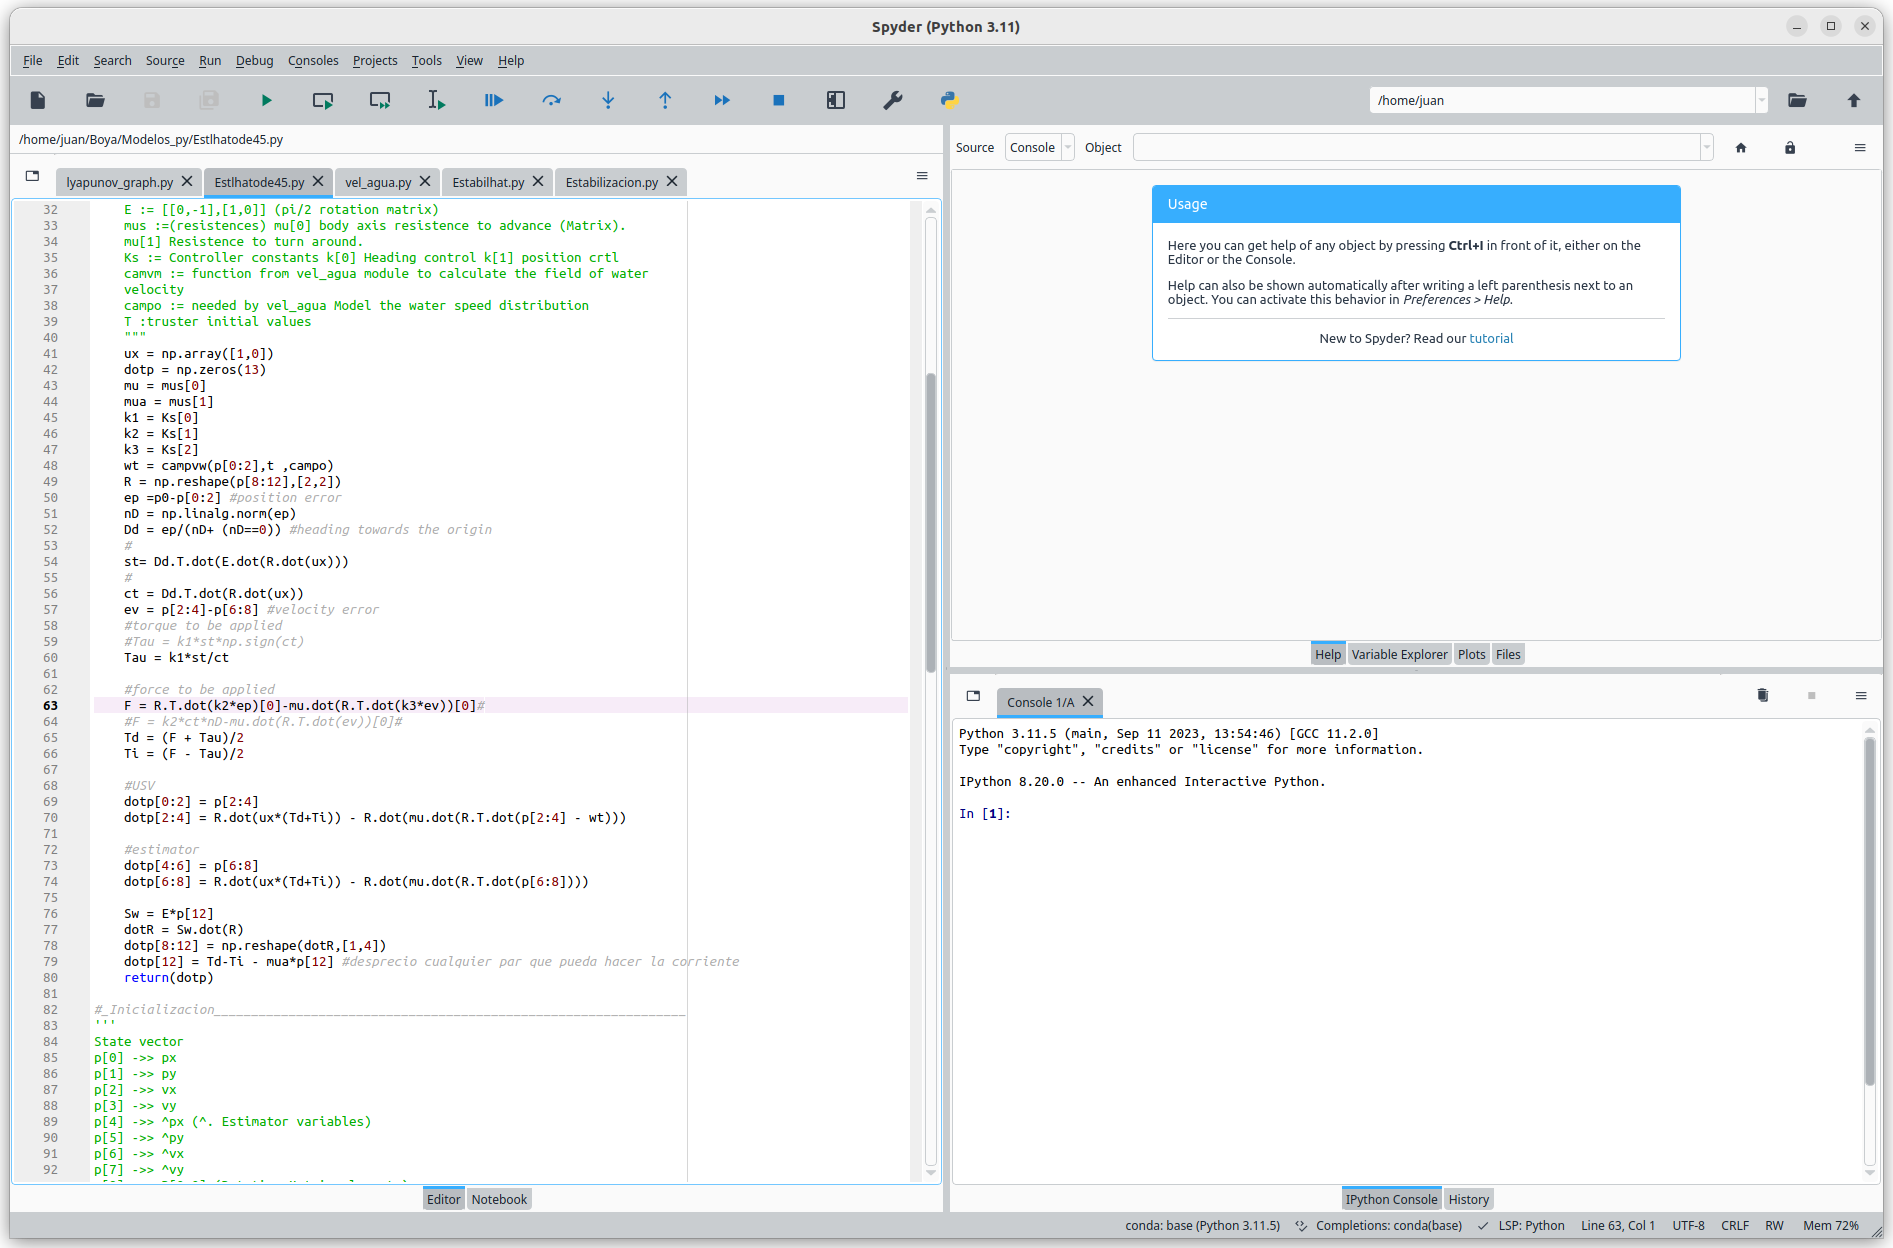
\includegraphics[width=14cm]{ide_n.png}
	\caption{Entorno de desarrollo integrado de Matlab}
	\label{fig:ide}
\end{figure}




\begin{figure}[h]
	\centering
		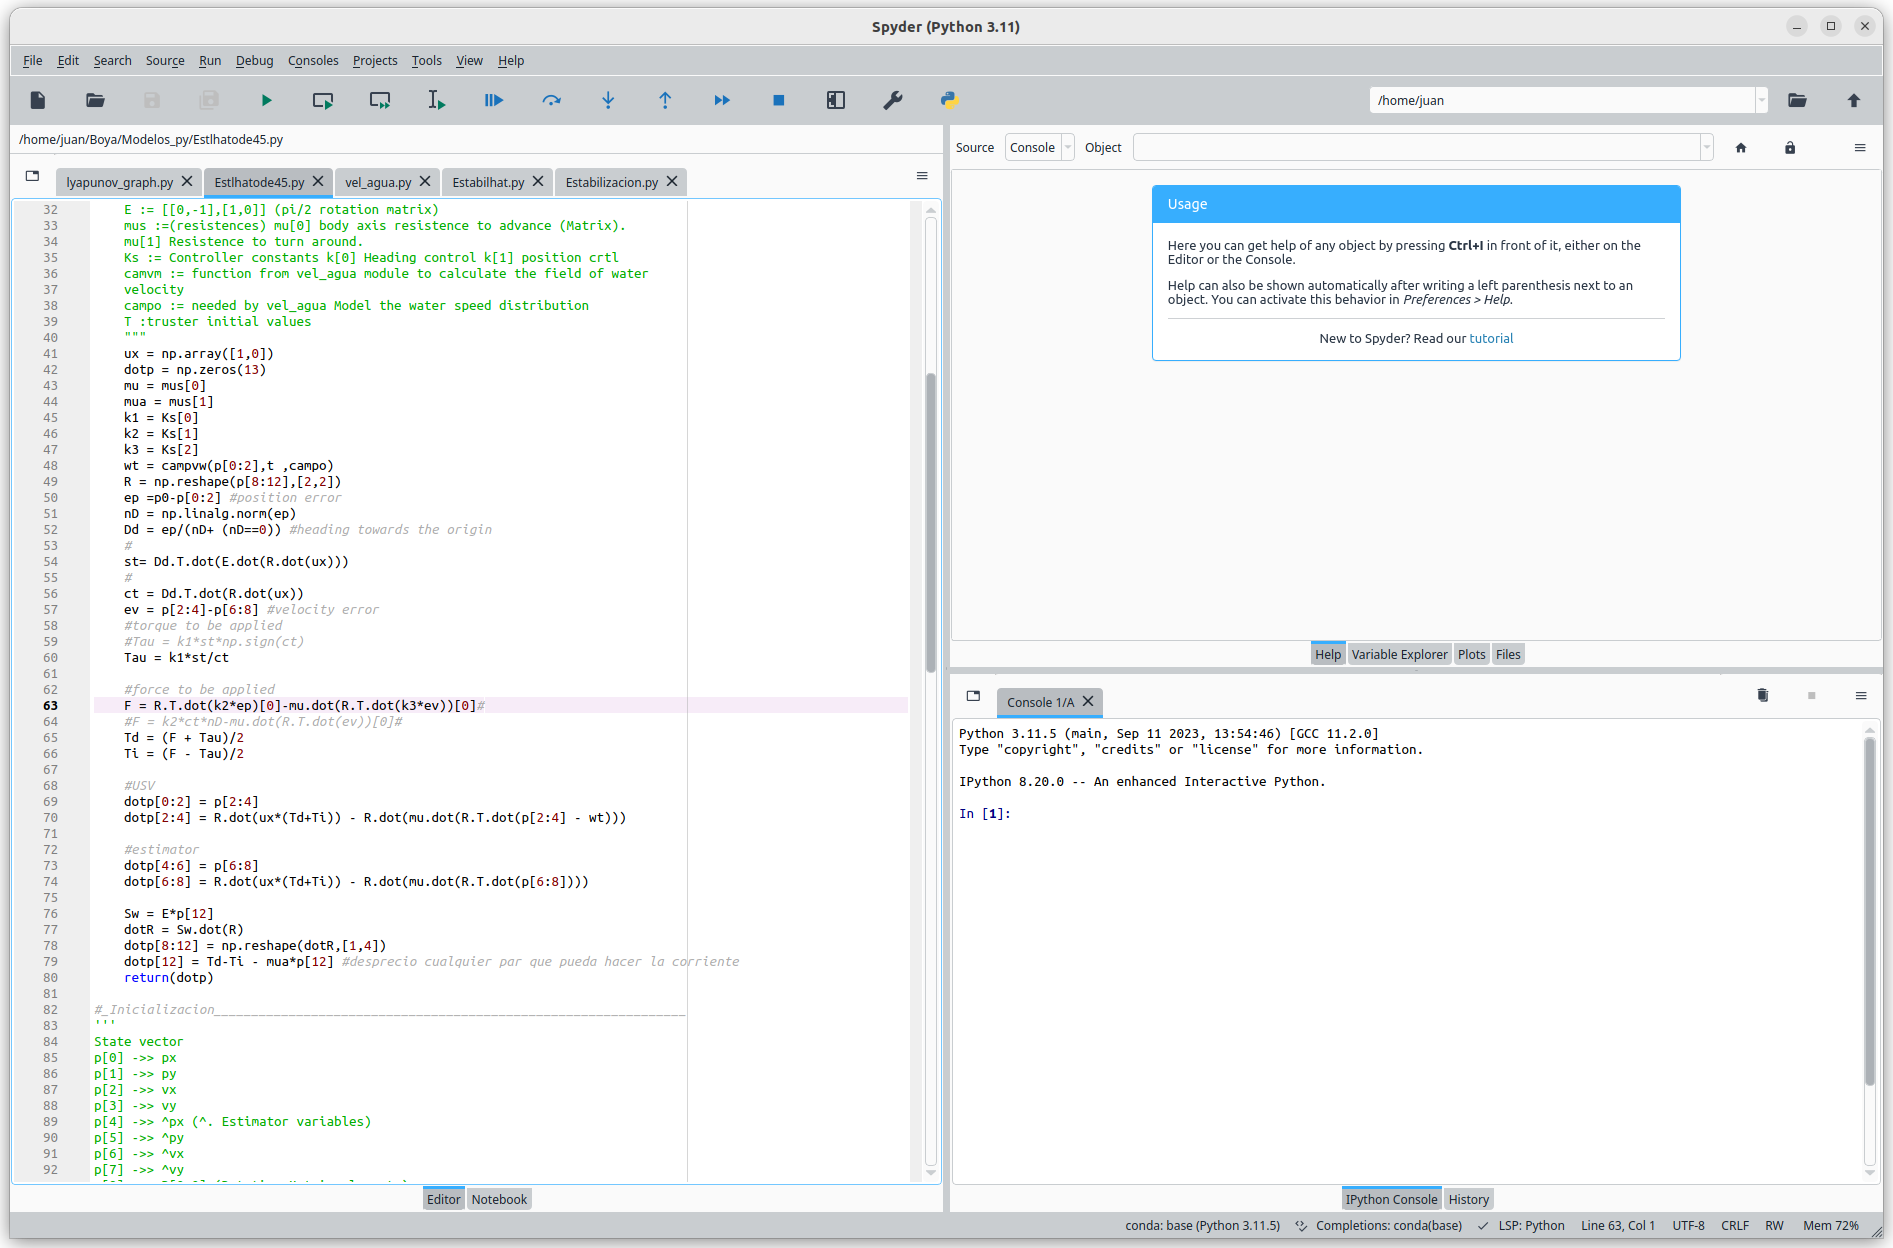
\includegraphics[width=14cm]{ide_n.png}
	\caption{Entorno de desarrollo integrado de Matlab}
	\label{fig:ide}
\end{figure}
FALTA EXPLICAR COMO SE INTALA EL PLUG-
IN THE JUPYTIR-NOTES.



Según como se configure, el IDE de Python puede mostrar un número mayor o menor de paneles y una disposición de los mismos distinta a la mostrada en la figura. La mejor manera de aprender estos y otros detalles del IDE es usarlo. Aquí nos centraremos solo en algunos aspectos fundamentales.

\subsection{La ventana de comandos de Matlab} \index{Matlab!ventana de Commandos}
De los paneles mostrados en la ventana de la figura \ref{fig:ide}, vamos a empezar examinando el situado en la parte inferior central. Se trata de la ventana de comandos (\emph{command window}) de Matlab.  \index{prompt} La ventana muestra el simbolo $>>$, que recibe el nombre de \emph{prompt} y, a continuación, una barra vertical $|$ parpadeante.  La ventana de comandos permite al usuario interactuar directamente con Matlab: Matlab puede recibir instrucciones directamente a través de la ventana de comandos, ejecuta las instrucciones recibidas, y devuelve los resultados de nuevo en la ventana de comandos. Veamos un ejemplo muy sencillo: si escribimos en la ventana de comandos:

\begin{verbatim}
>> a=18 + 3
\end{verbatim}

Matlab calcula la suma pedida, devuelve el resultado y, por último, vuelve a presentar el \emph{prompt}, para indicarnos que está preparado para recibir otro comando.

\begin{verbatim}
a =

    21

>> 
\end{verbatim}

De este modo, podemos emplear Matlab de un modo análogo a como emplearíamos una calculadora: realizamos una operación, obtenemos el resultado, realizamos otra operación, obtenemos el resultado  y así sucesivamente.
\subsection{Variables.} \index{Variable}
En el el ejemplo que acabamos de ver, Matlab calcula el resultado pedido, y lo presenta en pantalla usando la expresión, \begin{verbatim}
a =21
\end{verbatim} ¿Por qué hace falta escribir $a=18+3$ en lugar de escribir directamente $18+3$? La razón tiene que ver con el modo de trabajo de Matlab, y de otros lenguajes de alto nivel. Esto nos lleva al concepto de variable. 

Podemos ver una variable como una región de la memoria del computador, donde un programa guarda una determina información; números, letras, etc. Una característica fundamenta de una variable es su nombre, ya que permite identificarla. \index{Variable! nombre} Como nombre para una variable se puede escoger cualquier combinación de letras y números, empezando siempre con una letra, en el caso de Matlab\footnote{Como se verá más adelante, Matlab tiene un conjunto de nombres de instrucciones y comandos ya definidos. Se debe evitar emplear dichos nombres, ya que de hacerlo se pierde acceso al comando de Matlab que representan}. Se puede además emplear el signo "\_". Matlab distingue entre mayúsculas y minúsculas, por lo que si elegimos como nombres de variable Pino, PINO y PiNo, Matlab las considerará como variables distintas. 

\index{Variable! tipo} En algunos lenguaje, es preciso indicar al ordenador qué tipo de información se guardará en una determinada variable, antes de poder emplearlas. Esto permite manejar la memoria del computador de una manera más eficiente, asignando zonas adecuadas a cada variable, en función del tamaño de la información que guardarán. A este proceso, se le conoce con el nombre de \emph{declaración} de variables. En Matlab no es necesario declarar las variables antes de emplearlas.

El método más elemental de emplear una variable es asignarle la información para la que se creó. Para hacerlo, se emplea el símbolo de asignación \index{"= Símbolo de asignación} \index{Símbolo de asignación}, que coincide con el signo $=$ empleado en matemáticas. Como veremos más adelante la asignación en programación y la igualdad en matemáticas no representan exáctamente lo mismo. La manera de asignar directamente información a una variable es escribir el nombre de la variable, a continuación  el signo de asignación y, por último, la información asignada,
\begin{verbatim}
Nombre_variable = 4
\end{verbatim}  

Si escribimos en la ventana de comandos la expresión anterior y pulsamos el retorno de carro. Matlab devuelve el siguiente resultado:

\begin{verbatim}
>> Nombre_variable=4

Nombre_variable =

     4

>> 
\end{verbatim}  
Matlab ejecuta las instrucciones indicadas y nos confirma que ha creado en la memoria una variable \texttt{Nombre\_variable} y que ha guardado en  ella el número $4$. 

En Matlab podemos emplear el símbolo de asignación para construir variables que guarden distintos tipos de datos,

\begin{enumerate}
\item Enteros positivos y negativos
\begin{verbatim}
>> a=4
a =

     4

>>b=-4
b =

     -4

\end{verbatim}
\item Números con parte entera y parte decimal separadas por un punto, positivos y negativos.
\begin{verbatim}
>> a=13.4568
a =

   13.4568

>> b=-13.4568
b =

   -13.4568
\end{verbatim}


\item Números expresados como potencias de $10$ (la potencia de $10$ se representa con la letra e seguida del valor del exponente). 
\begin{verbatim}
>> f=3e10
f =

  3.0000e+010

>> g=-3e10
g =

 -3.0000e+010

>> h=3e-10
h =

  3.0000e-010

>> t=-3e-10
t =

 -3.0000e-010
 \end{verbatim}
 
\item Números complejos. Para indicar la parte imaginaria se puede emplear la letra \texttt{i} o la letra \texttt{j}.

\begin{verbatim}
>> s=2+3i
s =

   2.0000 + 3.0000i

>> w=4-5j
w =

   4.0000 - 5.0000i
\end{verbatim}

\item Caracteres, letras o números; manejados estos últimos como símbolos. Se indica a Matlab que se trata de un carácter escribiéndolo entre comillas simples,
\begin{verbatim}
>> p='a'
p =

a

>> k='1'
k =

1
\end{verbatim}

\item Cadenas de caracteres. 
\begin{verbatim}
>> m='hola amigos'
m =

hola amigos
\end{verbatim}

\end{enumerate}
 La forma que hemos visto de asignar un valor a una variable es la más sencilla pero no es la única. También podemos asignar un valor a una variable a partir de una expresión aritmética, como hemos visto antes. Ademas podemos asignar un valor a una variable copiando el contenido de otra variable:
\begin{verbatim}
>> a=18

a =

    18

>> b=a

b =

    18

>> 
\end{verbatim}
Por último, podemos asignar a una variable el valor de una función en un punto:
\begin{verbatim}
>> x=0
x =

     0

>> y=cos(x)
y =

     1

>> 
\end{verbatim}

La variable \texttt{y} contiene el valor de la función coseno en el punto \texttt{x=0}. Más adelante estudiaremos cómo manejar funciones en Matlab. 

Si escribimos directamente en la línea de comandos de Matlab, un número, una expresión algebraica o una función, sin asignarlas a una variable, Matlab crea automáticamente una variable para guardar el resultado, Así por ejemplo:
\begin{verbatim}
>> 3 + 5
ans =

     8

>> 
\end{verbatim}
Matlab guarda el resultado de la operación realizada: $3+5$, en la variable \texttt{ans}\index{ans, nombre de variable por defecto}.  Se trata del nombre de variable por defecto; es una abreviatura de al palabra inglesa \emph{answer} (respuesta).  En cualquier caso es recomendable asignar los resultados de las operaciones explícitamente a una variable.  La razón para ello tiene que ver con lo que llamaremos reasignación de variables.

Imaginemos que creamos en Matlab una variable asignándole un valor:

\begin{verbatim}
>> a=34

a =

    34

>> 
\end{verbatim}
Si a continuación, asignamos a esa misma variable el resultado de una operación,
\begin{verbatim}
>> a=12+5

a =

    17

>> 
\end{verbatim}
El valor inicialmente asignado a la variable \texttt{a} se pierde. Sencillamente hemos \emph{reasignado} a la variable un nuevo valor sobreescribiendo el anterior. Si en la línea de comandos escribimos operaciones sin asignar el resultado a una variable concreta, Matlab lo asignará a la variable \texttt{ans} pero esto significa que cada nueva operación reasigna su resultado a la variable \texttt{ans}, con lo que solo conservaremos al final el resultado de la última de las operaciones realizadas.

Es posible en Matlab crear una variable que no contenga nada. Para ello hay que emplear dos símbolos especiales: $[$ y $]$. Así, si escribimos en la línea de comandos:
\begin{verbatim}
>> variable_vacia=[]

variable_vacia =

     []

>> 
\end{verbatim}
obtenemos una variable que no contiene nada. Más adelante veremos la utilidad de hacerlo.

Hasta ahora, siempre que hemos realizado una operación en la ventana de comandos, Matlab nos ha \emph{respondido} escribiendo en pantalla el resultado de la misma. En muchas ocasiones, no nos interesa que Matlab nos muestre por pantalla el resultado de una operación; por ejemplo, porque se trata de un resultado intermedio, o porque es un resultado de gran tamaño y su visualización por pantalla no es útil y sin embargo sí que consume mucho tiempo. Podemos omitir la visualización por pantalla del resultado de una operación, si terminamos la operación, añadiendo al final un \emph{punto y coma} (\texttt{;}),

\begin{verbatim}
>> A=3+5;
>> B=A+1
B =

     9

\end{verbatim}
En la primera operación hemos añadido (\texttt{;}) al final de la línea, Matlab no muestra el resultado. Sin embargo, sí que ha realizado la operación pedida y guardado el resultado en la variable \texttt{A}. Por eso es posible emplearla en la segunda operación para crear la variable \texttt{B}.
\paragraph*{Recursión.} \index{Recursión} Hemos indicado antes cómo el símbolo de asignación $=$ en programación no coincide exactamente con la igualdad matemática. Un ejemplo claro de estas diferencias lo constituye la recursión. Esta se produce cuando la misma variable aparece a los dos lados del símbolo de asignación:
\begin{verbatim}
>> a=3

a =

     3

>> a=a+1

a =

     4
\end{verbatim} 
La expresión anterior no tiene sentido matemáticamente, ya que una variable no puede ser igual a sí misma más la unidad. Sin embargo, en programación, es  una sentencia válida; el ordenador toma el valor almacenado en la variable $a$, le suma $1$ y guarda el resultado en la variable $a$, sobreescribiendo el valor anterior.

La recursión se emplea muy a menudo en programación, entre otras aplicaciones, permite crear contadores, --variables que van incrementando o decrementando su valor progresivamente--  y permite ahorrar espacio de memoria cuando se realizan operaciones que requieren cálculos intermedios.

\paragraph*{El espacio de trabajo de Matlab \emph{Workspace}.} \index{Workspace}\index{Espacio de trabajo} Matlab guarda en memoria las variables que creamos en la ventana de comandos y las asocia a lo que se conoce como el espacio de trabajo de Matlab. Dicho espacio de trabajo contiene una relación de las variables creadas de modo que podamos volver a utilizarlas en la ventana de comandos. Uno de los paneles que el IDE de Matlab puede mostrarnos es precisamente el \emph{Workspace}. La figura \ref{fig:wsp} muestra dicho panel.  En el se muestran los nombres de las variables contenidas en el espacio de trabajo, así como información relativa a su valor, tamaño en memoria etc.


\begin{figure}[h]
	\centering
		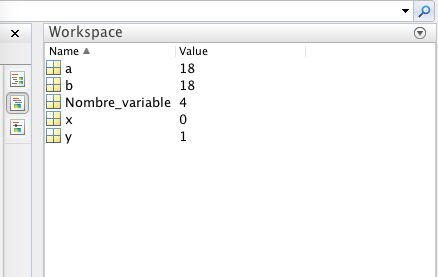
\includegraphics[width=8cm]{wsp2.png}
	\caption{El \emph{Workspace} de Matlab}
	\label{fig:wsp}
\end{figure}

Además del panel que acabamos de describir, es posible listar el contenido de las variables presentes en el \emph{Workspace} empleando dos comandos especiales de Matlab; se trata de los comandos \texttt{who} y \texttt{whos}. El primero de ellos nos devuelve en la ventana de comandos los nombres de las variables contenidas en el \emph{Workspace}. El segundo nos devuelve los nombres de las variables junto con información adicional sobre su contenido, tamaño, etc.
\begin{verbatim}
>> who

Your variables are:

Nombre_variable  b                y                
a                x                

>> whos
  Name                 Size            Bytes  Class     Attributes

  Nombre_variable      1x1                 8  double              
  a                    1x1                 8  double              
  b                    1x1                 8  double              
  x                    1x1                 8  double              
  y                    1x1                 8  double              

>> 
\end{verbatim}

Para eliminar una variable del \emph{Workspace}, se emplea el comando \texttt{clear}.  Si escribimos en la ventana de comandos el comando \texttt{clear}, seguido del nombre de una variables,  Matlab la elimina del \emph{Workspace}. Si escribimos el comando \texttt{clear}, sin añadir nada más, Matlab eliminará TODAS las variables contenidas en el \emph{Workspace}. 

\paragraph*{Formatos de visualización}\index{visualizacion de variables, formatos}\index{Variable! Formato}
Hemos visto en los ejemplos anteriores cómo al realizar una operación en Matlab, se nos muestra el resultado en la ventana de comandos. Además podemos examinar el contenido de cualquier variable contenida en el \emph{workspace} sin más que escribir su nombre en la ventana de comandos y pulsar la tecla \emph{intro}.

Matlab permite elegir la forma en que los resultados se presenta por pantalla. Para ello se emplea el comando \texttt{format}.  La siguiente tabla, resume los formatos más comúnmente empleados.

\begin{table}[h]
\caption{Formatos numéricos más comunes en Matlab}
\begin{tabular}{l l l }
\textbf{Comando} & \textbf{formato} & \textbf{Comentario}\\ \hline
\texttt{format short} & $12.3457$ & coma fija. Cuatro decimales\\
\texttt{format shortE} & $1.2346e+01$ & coma flotante. Cuatro decimales\\
\texttt{format long} & $12.345678901234500$ & coma fija. Quince decimales\\
\texttt{format longE} & $1.234567890123450e+01$ & coma flotante. Quince decimales\\ \hline 
\end{tabular}
\end{table}
\subsection{Vectores y matrices.} \index{Vectores! Definición en matlab} \index{Matrices! Definición en matlab} Una de las característica más interesantes de Matlab, es la posibilidad de crear fácilmente matrices. Se pueden crear de muchas maneras, la más elemental de todas ellas, emplea el operador de asignación $=$, y los símbolos especiales $[$, $]$, el punto y coma $;$ y la coma $,$. Las matrices se crean introduciendo los valores de sus elementos por filas, separados por comas o espacios. Una vez introducidos todos los elementos de una fila, se añade un punto y coma, o se pulsa la tecla \emph{intro}, y se añaden los elementos de la fila siguiente. El siguiente ejemplo muestra como crear una matriz de de dos filas y tres columnas:
\begin{verbatim}
 >> matriz23 =[ 1 3 4 ;3 5 -1]

matriz23 =

     1     3     4
     3     5    -1
\end{verbatim}
o también:
 \begin{verbatim}
  >> matriz23 =[ 1 3 4 
3 5 -1]

matriz23 =

     1     3     4
     3     5    -1
 \end{verbatim}

En el primer caso, se empleado el punto y coma para separar las filas y en el segundo se ha empleado la tecla \emph{intro}.  En ambos se emplea el símbolo $[$ para indicar a Matlab que queremos empezar a construir una matriz, y el símbolo $]$ para indicar a Matlab que hemos terminado de construirla. Una vez construida, Matlab nos devuelve en la ventana de comandos la Matriz completa. Matlab nos permite además emplear cada elemento de una matriz como si se tratase de una variable, es decir, se puede asignar  a los elementos de una matriz un valor numérico, el resultados de una operación o un valor guardado en otra variable:
\begin{verbatim}
>> a=1

a =

          1.00

>> b=2

b =

          2.00

>> mtr=[ a a+b a-b; 1 0.5 cos(0)]

mtr =

          1.00          3.00         -1.00
          1.00          0.50          1.00

>> 
\end{verbatim}

Matlab considera las matrices como la forma básica de sus variables, así para Matlab un escalar es una matriz de una fila por una columna. Un vector \emph{fila} de 3 elementos es una matriz de una fila por tres columnas y un vector \emph{columna} de tres elementos es una matriz de tres filas y una columna.

\paragraph*{Indexación.} \index{Indexación en matlab}Al igual que se hace en álgebra, Matlab es capaz de referirse a un elemento cualquiera de una matriz empleando índices para determinar su posición (fila y columna) dentro de la matriz.
\begin{equation*}
a=
\begin{pmatrix}
a_{11}&a_{12}&a_{13}\\
a_{21}&a_{22}&a_{23}\\
a_{31}&a_{32}&a_{33}
\end{pmatrix}
\end{equation*}

El criterio para referirse a un elemento concreto de una matriz, en Matlab es el mismo: se indica el nombre de la variable que contiene la matriz y a continuación, entre paréntesis y separados por una coma, el índice de su fila y después él de su columna:
 \begin{verbatim}
 >> a=[1 2 3; 4 5 6; 7 8 9]

a =

          1.00          2.00          3.00
          4.00          5.00          6.00
          7.00          8.00          9.00

>> a(1,2)

ans =

          2.00

>> a(2,1)

ans =

          4.00

>> 
 \end{verbatim}
 
Es interesante observar de nuevo cómo Matlab asigna por defecto el valor del elemento buscado a la variable \texttt{ans}. Como ya se ha dicho, es mejor asignar siempre una variable a los resultados, para asegurarnos de que no los perdemos al realizar nuevas operaciones:
\begin{verbatim}
>> a12=a(1,2)

a12 =

          2.00

>> a21=a(2,1)

a21 =

          4.00

>> 
\end{verbatim}
Ahora hemos creado dos variables nuevas que contienen los valores de los elementos $a_{12}$ y $a_{21}$ de la matriz $a$. 

Matlab puede seleccionar dentro de una matriz no solo elementos aislados, sino también submatrices completas. Para ello, emplea un símbolo reservado, el símbolo \emph{dos puntos} $:$. Este símbolo se emplea para recorrer valores desde un valor inicial hasta un valor final, con un incremento o paso fijo. La sintaxis es: \texttt{inicio:paso:fin}, por ejemplo podemos recorrer los números enteros de cero a 8 empleando un paso 2:
\begin{verbatim}
>> 0:2:8

ans =

             0          2.00          4.00          6.00          8.00

>> 
\end{verbatim}

El resultado nos da la lista de los números $0, 2, 4, 6, 8$.
Además, si no indicamos el tamaño del paso,  Matlab tomará por defecto un paso igual a uno. En este caso basta emplear un único símbolo \emph{dos puntos} para separar el valor de inicio del valor final:
 \begin{verbatim}
 >> 1:5

ans =

          1.00          2.00          3.00          4.00          5.00

>>
 \end{verbatim}
 
 Podemos emplear el símbolo \emph{dos puntos},\index{Indexación con el operador :} \index{": Operador de indexación} para obtener submatrices de una matriz dada. Así por ejemplo si construimos una matriz de cuatro filas por cinco columnas:
 \begin{verbatim}
 >> matriz=[1 2 4 5 6
3 5 -6 0 2
4 5 8 9 0
3 3 -1 2 0]

matriz =

          1.00          2.00          4.00          5.00          6.00
          3.00          5.00         -6.00          0.00          2.00
          4.00          5.00          8.00          9.00          0.00
          3.00          3.00         -1.00          2.00          0.00

>> 
 \end{verbatim}
 Podemos obtener el vector formado por los tres últimos elementos de su segunda fila:
 \begin{verbatim}
 >> fil=matriz(2,3:5)

fil =

         -6.00             0          2.00

>> 
 \end{verbatim}

 o la submatriz de tres filas por tres columnas formada por los elementos que ocupan las filas 2 a 4 y las columnas 3 a 5:
\begin{verbatim}
 >> subm=matriz(2:4,3:5)

 subm =

         -6.00          0                2.00
	          8.00          9.00             0  
         -1.00          2.00             0  

 >> 
\end{verbatim}

o el vector columna formado por su segunda columna completa:
\begin{verbatim}
>> matriz(1:4,2)

ans =

          2.00
          5.00
          5.00
          3.00

>> 
\end{verbatim} 

De hecho, si deseamos seleccionar todos los elementos en una fila o una columna, podemos emplear el símbolo \texttt{:} directamente sin indicar principio ni fin,

\begin{verbatim}

>> matriz(:,2)

ans =

          2.00
          5.00
          5.00
          3.00

>> matriz(3,:)
ans =

     4.00     5.00     8.00    9.00    0.00
\end{verbatim}
 
\label{index}A parte de la indexación típica del álgebra de los elementos de una matriz indicando su fila y columna, en Matlab es posible referirse a un  elemento de una matriz empleando un único índice. En este caso, Matlab cuenta los elementos por columnas, de arriba abajo y de izquierda a derecha, 

\begin{equation*}
A=
\begin{pmatrix}
a_1&a_4&a_7\\
a_2&a_5&a_8\\
a_3&a_6&a_9
\end{pmatrix}
\end{equation*}

Así por ejemplo, en una matriz $A$ de $3$ filas y $4$ columnas, 
\begin{verbatim}
>> A=[3 0 -1 0; 2 1 5 7; 1 3 9 8]
A =

     3     0    -1     0
     2     1     5     7
     1     3     9     8
\end{verbatim}
las expresiones,
\begin{verbatim}
>> A(2,3)

and =
     5
\end{verbatim}
y
\begin{verbatim}
>> A(8)

ans =
     5
\end{verbatim} 
hacen referencia al mismo elemento de la matriz $A$. 

Aunque el concepto de función no se explicará hasta la sección \ref{funciones}, vamos a hacer uso de un par de funciones sencillas relacionadas con el tamaño de una matriz. En primer lugar, tenemos la función \texttt{length}; esta función nos calcula el número total de elementos que contiene un vector, sea este fila o columna.  Así, si tenemos un vector guardado en la variable  \texttt{a}, para saber su longitud escribimos en matlab el nombre de la función seguida del nombre de la variable entre paréntesis \texttt{length(a)},

\begin{verbatim}
>> a = [ 1 -2 0 6 8]
a =

     1    -2     0     6     8
>> length(a)

ans =

     5

>> 
\end{verbatim} 

La segunda función es la función \texttt{size}, esta función permite obtener el número de filas y columnas de una matriz o vector. \texttt{size} nos da como resultado de aplicarlo a una matriz un vector cuyo primer elemento es el número de filas de la matriz, y cuyo segundo elemento el número de columnas,

\begin{verbatim}
>> A = [1 3 4 -5; 2 3 0 -2; -2 1 7 7]
A =

     1     3     4    -5
     2     3     0    -2
    -2     1     7     7

>> size(A)

ans =

     3     4
\end{verbatim}  


\subsection{Estructuras y células}\index{Estructuras}\index{Células (cells)}
Se trata de dos tipos de variables especiales. Ambas comparten la propiedad de poder combinar dentro de sí variables de distintos tipos.

\paragraph*{Estructuras.} Una estructura es una variable que guarda la información divida en campos. Por ejemplo, si escribimos en la ventana de matlab,

\begin{verbatim}
>> est.nombre='Ana'
est = 
    nombre: 'Ana'
>> est.edad=25
est = 
    nombre: 'Ana'
      edad: 25
\end{verbatim}

obtenemos una estructura con dos campos, el primero de ellos es el campo \texttt{nombre}, y guarda dentro una cadena de caractéres \texttt{'Ana'}, el segundo es el campo \texttt{edad} y guarda dentro el valor \texttt{25}. La estructura que acabamos de definir es una sola variable llamada \texttt{est} y podemos aplicar cualquier comando de matlab cuyo resultado no dependa del contenido específico de la variable. Podemos copiarla en otra estructura,

\begin{verbatim}
>> est2=est
est2 = 
    nombre: 'ana'
      edad: 25
\end{verbatim}
podemos borrarla,

\begin{verbatim}
>> clear est
>> who
Your variables are:
est2  
>> 
\end{verbatim}

No podemos realizar sobre ella, como un todo, operaciones aritméticas o relacionales, pero sí sobre sus campos,

\begin{verbatim}
>> x=est.edad+12
x =
    37
\end{verbatim} 

El número de campos de una estructura puede aumentarse añadiendo a su nombre, el nombre del nuevo campo separado por un punto y asignando un valor o una variable a dicho campo.

\begin{verbatim}
>> est.campo_nuevo=[1 2;3 4; 6 7]
est = 
         nombre: 'ana'
           edad: 25
    campo_nuevo: [3x2 double]
    >> y=[1 2 3]
y =
     1     2     3
>> est.campo_nuevo2=y
est = 
          nombre: 'ana'
            edad: 25
     campo_nuevo: [3x2 double]
    campo_nuevo2: [1 2 3]
\end{verbatim}
 
 Podemos tambien eliminar campos de una estructura mediante el comando \texttt{rmfield},
 
 \begin{verbatim}
 >> est=rmfield(est,'edad')
est = 
          nombre: 'ana'
     campo_nuevo: [3x2 double]
    campo_nuevo2: [1 2 3]
 \end{verbatim}
 
Por último, una estructura nos permite definir y utilizar varios niveles de campos. Para ello, basta ir definiendo los nombres de los campos de un nivel separados por un punto del nombre del nivel anterior, 

\begin{verbatim}
>> multinivel.datos_personales.nombre='Ana'
multinivel = 
    datos_personales: [1x1 struct]
>> multinivel.datos_personales.primer_apellido='Jiménez'
multinivel = 
    datos_personales: [1x1 struct]
>> multinivel.datos_personales.segundo_apellido='Lasarte'
multinivel = 
    datos_personales: [1x1 struct]
>> multinivel.domicilio.calle='Ponzano'
multinivel = 
    datos_personales: [1x1 struct]
           domicilio: [1x1 struct]
>> multinivel.domicilio.numero=724
multinivel = 
    datos_personales: [1x1 struct]
           domicilio: [1x1 struct]
>> multinivel.valor=[3 4 5; 3.5 2 3]
multinivel = 
    datos_personales: [1x1 struct]
           domicilio: [1x1 struct]
               valor: [2x3 double]
\end{verbatim}

La información se encuentra ahora estructurada en niveles. Así por ejemplo,

\begin{verbatim}
>> multinivel.domicilio
ans = 
     calle: 'Ponzano'
    numero: 724
\end{verbatim}

Me devuelve el contenido del campo \texttt{domicilio} que es a su vez una estructura formada por dos campos  \texttt{calle} y  \texttt{numero}. La información queda estructurada en niveles que pueden ramificarse tanto como se desee. Para obtener la información contenida al final de una rama, es preciso indicar todos los campos que se atraviesan hasta llegar a ella,

\begin{verbatim}
>> multinivel.datos_personales.segundo_apellido
ans =
Lasarte
\end{verbatim}

Matlab tiene definidas funciones propias para conseguir un manejo eficiente de las estructuras. A parte de la función \texttt{rmfield} de la que hemos hablado anteriormente, cabe destacar la función \texttt{struct} que permite crear directamente una estructura. Su sintaxis es,

\begin{verbatim}
 s= struct('field1', values1, 'field2', values2, ...)
\end{verbatim}

donde \texttt{s} representa el nombre de la estructura, \texttt{field1},\texttt{field2}, etc son los nombres correspondientes a cada campo, introducidos entre comillas, y \texttt{values1}, etc los valores contendidos en cada campo. Para un conocimiento más profundo del uso de las estructuras se aconseja consultar la ayuda de Matlab.

\paragraph*{Células.} Las células, \emph{cells} en Matlab, son objetos que almacenan datos de diversos tipos en una misma variable. A diferencia de las estructuras, las células no expanden un árbol de campos sino que guardan cada dato en una "celda".  Para referirse a una celda concreta, empleamos un índice, de modo análogo a como hacemos con un vector.  Para construir una célula, procedemos de modo análogo a como hacemos con un vector, pero en lugar de emplear corchetes como delimitadores, empleamos llaves. Así, por ejemplo,

 \begin{verbatim}
 >> a={[1 2 3; 4 5 6; 7 8 9],'cadena', -45;'pepe', [1 2 3], 'cadena2'}
a = 
    [3x3 double]    'cadena'        [    -45]
    'pepe'          [1x3 double]    'cadena2'
 \end{verbatim}

Hemos creado una célula \texttt{a}, cuyos elementos son, una matriz $3\times 3$, la cadena de caracteres \texttt{cadena}, el número $-45$, otra cadena de caracteres \texttt{pepe}, el vector $[1,2,3]$ y una última cadena de caracteres \texttt{cadena2}.

Los elementos separados por espacios o por comas simples, pertenecen a la misma fila dentro de la célula. Los elementos pertenecientes a distintas filas están separados por un punto y coma.  Podemos obtener el tamaño de la célula ---su número de filas y columnas--- empleando el comando \texttt{size} , igual que hicimos para el caso de vectores o matrices,

\begin{verbatim}
>> size(a)
ans =
     2     3
\end{verbatim}

Y podemos referirnos a una celda cualquiera de la célula, y obtener su contenido indicando entre llaves la fila y la columna a la que pertenece. Así por ejemplo, para obtener el vector $[1,2,3]$ de la célula \texttt{a} del ejemplo anterior hacemos,
\begin{verbatim}
>> vector=a{2,2}
vector =
     1     2     3
\end{verbatim}

Las celdas, de modo análogo a como sucedía con las estructuras, nos permiten agrupar datos de distinto tipo empleando una sola variable. Además, el hecho de que los datos ester ordenados por celdas en filas y columna, hace sencillo que se puede acceder a ellos.
 
\section{Entrada y salida de Datos}\index{Datos! Entrada y Salida}
Matlab posee una amplia colección de métodos para importar datos desde y exportar datos a un fichero. A continuación describimos algunos de los más usuales.

\subsection{Exportar e importar datos en Matlab} \label{fpf}

\paragraph*{Datos en formato propio de Matlab}
Matlab posee un formato de archivo propio para manejar sus datos. Los archivos de datos propios de Matlab, emplean la extensión \texttt{.mat}.


Si tenemos un conjunto de variables en el \emph{workspace}, podemos guardarlas en un fichero empleando el comando \texttt{save}, seguido del nombre del fichero donde queremos guardarlos. No es preciso incluir la extensión \texttt{.mat}, Matlab la añade automáticamente:
\begin{verbatim}
>> save datos
\end{verbatim}
Matlab creará en el directorio de trabajo un nuevo fichero \texttt{datos.mat} en el que quedarán guardadas todas las variables contenidas en el \emph{workspace}.  Los ficheros \texttt{.mat} generados por Matlab están escritos en binario. No se puede examinar su contenido empleando un editor de textos. Matlab almacena toda la información necesaria ---nombre de las variables, tipo, etc--- para poder volver a reconstruir las variables en el \emph{workspace} tal y como estaban cuando se generó el archivo.


Es posible guardar tan solo algunas de las variables contenidas en el \emph{workspace} en lugar de guardarlas todas. Para ello, basta añadir al comando \texttt{save}, detrás del nombre del archivo, el nombre de las variables que se desean guardar, separadas entre sí por un espacio
\begin{verbatim}
>>save datos1 A  matriz_1 B 
\end{verbatim}
La instrucción anterior guarda en un archivo ---llamado datos1.mat--- las variables \texttt{A}, \texttt{matriz1} y \texttt{B}.


Los datos contenidos en cualquier fichero \texttt{.mat} generado con el comando \texttt{save} de Matlab, pueden volver a cargarse en el \emph{workspace} empleando el comando \texttt{load}, seguido del nombre del fichero cuyos datos se desean cargar:
\begin{verbatim}
load datos.mat
\end{verbatim}
 carga en el \emph{workspace} las variables contenidas en el fichero \texttt{datos.mat}, la extensión del fichero puede omitirse al emplear la función \texttt{load}. Si conocemos los nombres de las variables contenidas en un archivo \texttt{.mat}, podemos cargar en Matlab solo una o varias de las variables contenidas en el archivo, escribiendo sus nombres, separados por espacios, detrás del nombre del archivo: 
\begin{verbatim}
>>load datos A G matriz1
\end{verbatim}
 cargará tan solo las variables \texttt{A}, \texttt{G} y \texttt{matriz1}, de entre las que contenga el ficheros \texttt{datos.mat}

\paragraph*{Datos en Formato ASCII} \index{Datos!Formato ASCII}\index{ASCII, Formato de datos}e puede emplear también el comando \texttt{save} para exportar datos en formato ASCII. Pare ello es preciso añadir al comando modificadores,
\begin{verbatim}
>>save datos.txt A -ASCII
\end{verbatim}

Este comando guardará la variable \texttt{A} en el fichero \texttt{datos.txt}. Matlab no añade ninguna extensión por defecto al nombre del fichero cuando empleamos el comando \texttt{save} con el modificador \texttt{-ASCII}. En este caso, hemos añadido explícitamente la extensión \texttt{.txt}, esto facilita que el archivo resultante se pueda examinar luego empleando un sencillo editor de texto o una hoja de cálculo.


Cuando se exportan datos desde Matlab en formato ASCII, Matlab guarda tan solo los valores numéricos contenidos en las variables, pero no los nombres de éstas. Por otro lado, guarda tan solo ocho dígitos, por lo que habitualmente se pierde precisión. Es posible guardar  datos en formato ASCII, conservando toda la precisión, si añadimos al comando \texttt{save} el modificador \texttt{-DOUBLE}, 
\begin{verbatim}
>>save nombre_Archivo matriz_1, matriz2, ... -ASCII -DOUBLE
\end{verbatim}


Supongamos que en \emph{workspace} tenemos guardada la siguiente matriz,

\begin{equation*}
a=
\begin{pmatrix}
1.300236890000000e+000&3.456983000000000e+000&4.321678000000000e+006\\
4.000230000000000e+003&1.245677000000000e+001&1.231565670000000e+002
\end{pmatrix}
\end{equation*}
Si ejecutamos en Matlab, 
\begin{verbatim}
>>save datos.txt a -ASCII
\end{verbatim}

El fichero resultante tendrá el aspecto siguiente,
\begin{verbatim}
   1.3002369e+00   3.4569830e+00   4.3216780e+05
   4.0002300e+03   1.2456770e+01   1.2315657e+02
\end{verbatim}

es decir, los elementos de una misma fila de la matriz \texttt{a} se guardan en una fila separados por espacios, las filas de la matriz se separan empleando retornos de carro ---cada una ocupa una línea nueva--- y los valores cuyos dígitos significativos exceden de 8 se han truncado, redondeando el último dígito representado. Este último es el caso de los elementos $a_{11}$ y $a_{33}$ de la matriz del ejemplo.

Cuando se guardan varias variables o todo el \emph{workspace} en un mismo fichero con formato ASCII, es preciso tener en cuenta que Matlab se limitará a guardar los contenidos de las variables, uno debajo de otro, en el orden en que las escribamos detrás del comando \texttt{save} (en el caso de que guardemos todas las variables del \emph{workspace} las guardará una debajo de otra por orden alfabético), por lo que resulta difícil distinguir las variables originales.
Así por ejemplo, si tenemos en el \emph{workspace} las variables,
 \begin{equation*}
 A=
 \begin{pmatrix}
3&5\\
2&1\\
8&0
\end{pmatrix}
a=
\begin{pmatrix}
1&3&4\\
4&5.6&2\\
3&0&1
\end{pmatrix}
c=
\begin{pmatrix}
3&2
\end{pmatrix}
\end{equation*}
La orden,
\begin{verbatim}
>>save datos.txt c a A -ASCII
\end{verbatim}

produce el un archivo con el siguiente contenido,
\begin{verbatim}
   3.0000000e+00   2.0000000e+00
   1.0000000e+00   3.0000000e+00   4.0000000e+00
   4.0000000e+00   5.6000000e+00   2.0000000e+00
   3.0000000e+00   0.0000000e+00   1.0000000e+00
   3.0000000e+00   5.0000000e+00
   2.0000000e+00   1.0000000e+00
   8.0000000e+00   0.0000000e+00
\end{verbatim}

El comando \texttt{load}, presenta algunas limitaciones para cargar datos contenidos en un fichero ASCII. Solo funciona correctamente si el contenido del fichero puede cargarse en una única matriz, es decir, cada fila de datos en el fichero debe contener el mismo número de datos. Así, en el ejemplo anterior, los datos guardados en el fichero \texttt{datos.txt}, no pueden volver a cargarse en Matlab usando el comando load.

Para el caso de un fichero cuyos contenido pueda adaptarse a una matriz, el comando load carga todos los datos en una única matriz a la que asigna el nombre del fichero sin extensión.

\paragraph*{Lectura y escritura de datos con formato} \index{Datos!Lectura y escritura}

Matlab puede también escribir y leer datos, empleando formatos y procedimientos similares a los de el lenguaje C. Para ello, es preciso emplear varios comandos\footnote{Lo que se ofrece a continuación es solo un resumen del uso de los comandos y formatos más frecuentes. Para obtener una información completa, consultar la ayuda de Matlab.}:

En primer lugar es preciso crear ---o si ya existe abrir--- el archivo en que se quiere guardar o del que se quieren leer los datos. En ambos casos se emplea para ello el comando \texttt{fopen}. La sintaxis de este comando es de la forma,
\begin{verbatim}
fid=fopen(nombre de fichero, permisos)
\end{verbatim} 
El nombre del fichero debe ser una cadena de caracteres, es decir, debe ir escrito entre apóstrofos. Hay al menos ocho tipos de permisos distintos. Aquí describiremos tan solo tres de ellos, \texttt{'w'} ---\emph{write}--- abre o crea un archivo con permiso de escritura. Si el archivo ya existía su contenido anterior se sobreescribe. Si se quiere añadir datos a un archivo sin perder su contenido se emplea el permiso \texttt{'a'} ---\emph{append}--- los nuevos datos introducidos se escriben al final del fichero, a continuación de los ya existentes. \texttt{'r'} ---\emph{read}--- permiso de lectura, es la opción por defecto, permite leer el contenido de un archivo. Cuando se trabaja en el sistema operativo \emph{Windows}, es común emplear los permisos en la forma \texttt{'wt'} y \texttt{'rt'}, de este modo, los archivos se manejan en el denominado formato 'texto'. La variable \texttt{fid}, es un identificador del fichero abierto y es también la forma de referirnos a él ---en un programa, o en la línea de comandos--- mientras permanece abierto.

Supongamos que hemos abierto ---o creado--- un archivo para escribir en él, datos contenidos en el \emph{workspace}, 
\begin{verbatim}
fichero1=fopen('mi_fichero','wt') 
\end{verbatim}

Para escribir en él emplearemos el comando fprintf. La sintaxis de este comando necesita un identificador de archivo --en nuestro caso sería fichero1--, un descriptor del formato con el que se desean guardar los datos y el nombre de la variable que se desea guardar.
\begin{verbatim}
control=fprintf(fichero1,formato,nombre_de_variable,...)
\end{verbatim} 
Los descriptores de formato se escriben entre apóstrofos. Empiezan siembre con el carácter \texttt{\%}, seguido de un número con formato \emph{e.d}. Donde \emph{e} recibe el nombre de anchura de campo  y \emph{d} recibe el nombre de precisión. Por último se añade un carácter, conocido como carácter de conversión, que permite ajustar el formato numérico de los datos. Los más usuales son: \texttt{f} ---notación de punto fijo---, \texttt{e} ---notación exponencial--- y \texttt{g} ---la notación que resulte más compacta de las dos anteriores---.  La anchura de campo representa en número mínimo de caracteres que se emplearán para representar el número.  La precisión depende del carácter de conversión; para \texttt{f} y  \texttt{e}, representa el número de dígitos  a la derecha del punto decimal, para  \texttt{g} el número de dígitos significativos.

Aquí hemos incluido solo los caracteres de conversión más usuales para el caso de datos numéricos. Cabe añadir que para el caso de una cadena de caracteres se emplea como carácter de conversión la letra $s$.  Por ejemplo:

\begin{verbatim}
>>A='mi cadena de caracteres'
>>num=fprinf(fid,'%s', A)
\end{verbatim}
Escribe  el texto contenido en el vector \texttt{A} en el archivo indicado por \texttt{fid}.
 
Matlab, almacena los datos consecutivamente uno detrás de otro. Si se trata de matrices, los va leyendo por columnas y una variable tras otra en el orden en que se hayan introducido al llamar a la función \texttt{fprintf}. Para separar entre sí los datos se puede añadir a los descriptores de formatos, espacios y también caracteres de escape como Retornos de carro \texttt{\textbackslash r}, indicadores de salto de línea \texttt{\textbackslash n} o tabuladores \texttt{\textbackslash t}, entre otros.

Por ejemplo, supongamos que tenemos en Matlab las siguiente matrices

 \begin{equation*}
 A=
 \begin{pmatrix}
3.25&5.22\\
23.1&130.5\\
8&0
\end{pmatrix}
a=
\begin{pmatrix}
1.2345&3.0879&4234.2\\
40&5000.6&223\\
3&0&1
\end{pmatrix}
c=
\begin{pmatrix}
30&2
\end{pmatrix}
\end{equation*}

Si empleamos,
\begin{verbatim}
>>num=fprinf(fid,'%2.1f', A, a, c)
\end{verbatim}

Los datos se guardarán en el archivo indicado por \texttt{fid} en la siguiente forma:
\begin{verbatim}
3.223.18.05.2130.50.01.240.03.03.15000.60.04234.2223.01.030.02.0
\end{verbatim}

Guardados en este formato resulta bastante difícil reconocerlos. Si probamos,
\begin{verbatim}
>>num=fprinf(fid,'%2.1f ', A, a, c)
\end{verbatim}

El resultado sería,
\begin{verbatim}
3.2 23.1 8.0 5.2 130.5 0.0 1.2 40.0 3.0 3.1 5000.6 0.0 4234.2 223.0 1.0 30.0 2.0
\end{verbatim}

El formato es de punto fijo y los datos aparecen separados por un espacio ---nótese que en el descriptor de formato se ha incluido un espacio entre la f y el apóstrofo---. Los datos de las tres matrices aparecen uno detrás de otro, y se han ido escribiendo en el archivo por columnas

Si cambiamos de nuevo el descriptor de formato,
\begin{verbatim}
>>num=fprinf(fid,'%2.3g\n', A, a c)
\end{verbatim}
obtendremos,
\begin{verbatim}
3.25
23.1
 8
5.22
130
 0
1.23
40
 3
3.09
5e+03
 0
4.23e+03
223
 1
30
\end{verbatim}
Matlab elige el formato más compacto para cada dato, y guarda cada dato en una fila nueva, debido al término \texttt{\textbackslash n} introducido al final del descriptor.

Por último indicar que es posible emplear varios descriptores consecutivos, en cuyo caso, Matlab los aplica a cada dato consecutivamente, cuando ha terminado con la lista de descriptores, comienza de nuevo por el principio.

Por ejemplo, 

\begin{verbatim}
>>num=fprinf(fid,'%2.3g %2.3g %2.3g\n', a)
\end{verbatim}
Guarda los datos contenidos en \texttt{a} como,
\begin{verbatim}
1.23 40 3.09
5e+03 4.23e+03 223
\end{verbatim}

Es decir cada tres datos cambia a una línea nueva. Por supuesto, podríamos hacer que los datos se guardaran con un formato distinto en cada caso,
\begin{verbatim}
>>num=fprinf(fid,'%2.3g %3f %2.3f\n', a)

1.23 40.000000 3.088
5e+03 4234.200000 223.000
\end{verbatim}

Por último indicar, que si se emplea el comando \texttt{fprintf} sin emplear un  identificador de archivo o empleando como identificador el valor $1$. Matlab escribe el resultado directamente en la ventana de comandos con el formato deseado.

Por ejemplo, 
\begin{verbatim}
>>B = [8.8  7.7; 8800  7700];
>>fprintf(1, 'X is %6.2f metros o %8.3f mm\n', 9.9, 9900, B)
\end{verbatim}
Mostrará en la ventana de comandos las siguientes líneas:
\begin{verbatim}
X is 9.90 metros o 9900.000 mm
X is 8.80 metros o 8800.000 mm
X is 7.70 metros o 7700.000 mm
\end{verbatim}


Para cargar archivos desde un fichero que contiene datos en binario, se emplea el comando \texttt{fscanf}. Su uso es similar al de \texttt{fprintf}, pero ahora los datos pasarán desde el fichero donde están guardados a una matriz.

\begin{verbatim}
>>A=fscanf(pid,'%f')
\end{verbatim}

El comando \texttt{fscanf}, admite como parámetros  el número máximo de datos que se leerán del fichero,
\begin{verbatim}
a=fscanf(fid,'%5.2f',M)
\end{verbatim}
Lee como máximo M datos del fichero y los guarda en un vector \texttt{a}. Es posible dar a los datos formato de matriz, mediante dos parámetros (fila y columna),
\begin{verbatim}
a=fscanf(fid,'%5.2f',[M,N])
\end{verbatim}
Ahora creará una matriz \texttt{a} de M filas por N columnas. Matlab irá cogiendo los datos del fichero, por columnas hasta rellenar la matriz.

Es posible dar al segundo parámetro el valor \texttt{inf}. De este modo, Matlab creará una matriz de \texttt{M} filas y el número de columnas necesario para cargar todos los datos del fichero. (Si faltan elementos para completar la matriz resultante, Matlab rellena los huecos con ceros.)
Por último, una vez que se han escrito o leído datos en el fichero es preciso cerrarlo correctamente empleando el comando \texttt{fclose}, la sintaxis de este comando solo precisa que se incluya el identificador del fichero que se quiere cerrar,
\begin{verbatim}
>>fclose(fid)
\end{verbatim}

\paragraph*{Herramienta de importación de datos}\index{Datos! Importación}
Matlab posee una herramienta especial para importar datos. Con ella, es posible cargar en Matlab datos de muy diverso tipo, no sólo numéricos sino también imágenes, sonido, etc. Una de las ventajas de esta herramienta es que reconoce directamente ---entre otros--- los archivos creados por las hojas de cálculo.
\begin{figure}[h]
	\centering
		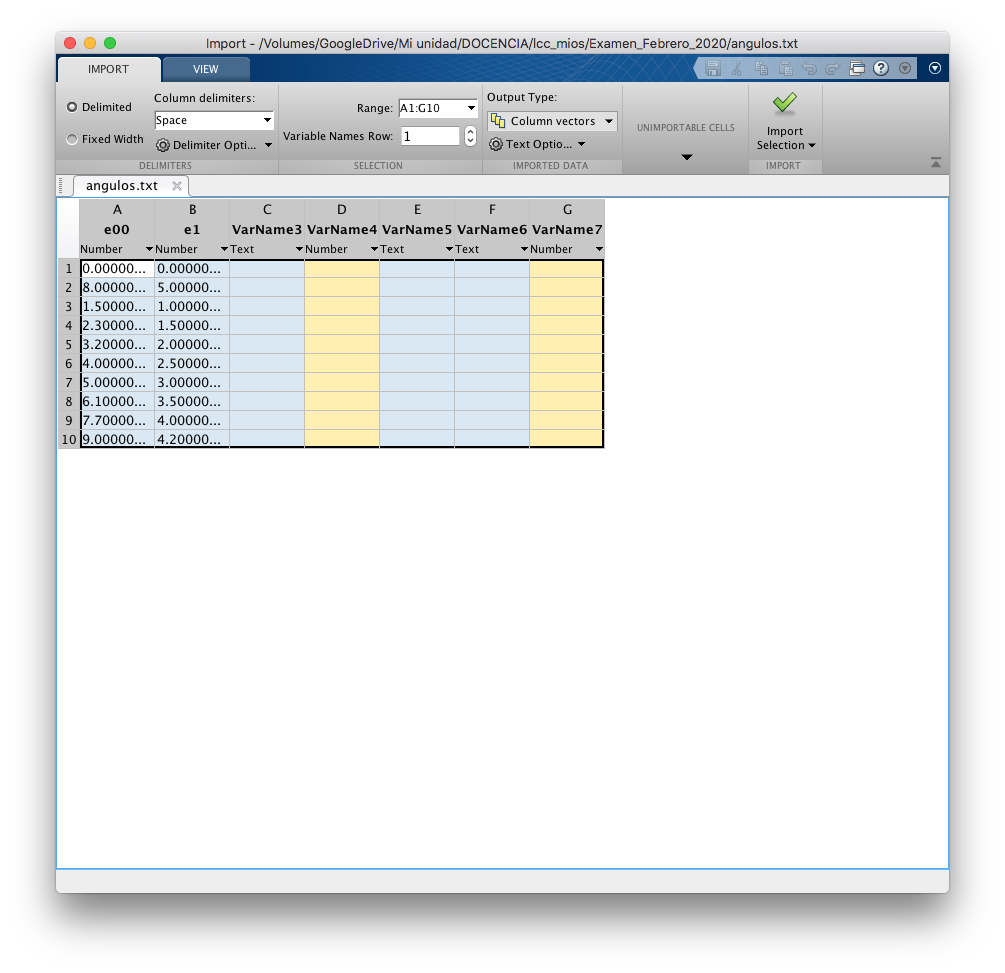
\includegraphics[width=10cm]{Wizard1.png}
	\caption{Aspecto de la herramienta de importación de datos}
	\label{fig:wizard}
\end{figure}

Para abrir en Matlab la herramienta de importación, basta pulsar en la pestaña \emph{home}, situada en la parte superior del IDE de Matlab,   el botón \emph{Import Data}. Matlab abre entonces una ventana que nos permite navegar por el árbol de directorio y seleccionar el archivo del que deseamos importar los datos. Una vez seleccionado, Matlab abre la ventana mostrada en la imagen \ref{fig:wizard}. 
Se trata de un programa especial ---\emph{import wizard}--- que sirve para guiar al usuario en el proceso de cargar las variables contenidas en el fichero en el \emph{workspace} de Matlab.

\section{Operaciones aritméticas, relacionales y lógicas}\index{Operaciones}

\subsection{Operaciones aritméticas}\index{Operaciones!Aritméticas}
 Una vez que sabemos como crear o importar variables en Matlab, vamos a ver como podemos realizar operaciones aritméticas elementales con ellas. La sintaxis es muy sencilla, y podemos sintetizarla de la siguiente manera:
\begin{equation*}
resultado=operando_1 operador_1 operando_2 operador_2 operando_3 \cdots operando_{n-1} operador_n
\end{equation*}
Es decir basta concatenar los operadores con los operandos y definir una variable en la que guardar el resultado. Por ejemplo,
\begin{verbatim}
>>x=1; y=2; z=3; q=x+y+z
>>z=6
\end{verbatim}
En este caso los operandos son las variables \texttt{x}, \texttt{y}, \texttt{z}, el operador, que se repite dos veces es el símbolo \texttt{+} que representa la operación suma y \texttt{q} es la variable en la que se guarda el resultado, en este caso, de la suma de las tres variables anteriores.

Los operadores aritméticos disponibles en Matlab cubren las operaciones aritméticas habituales, pero hay que recordar que Matlab considera sus variables como matrices. Por lo tanto, las operaciones definidas Matlab las considera por de defecto operaciones entre matrices. La tabla \ref{tabop} contiene los operadores definidos en  Matlab.

\begin{table}[h]
\caption{Operadores aritméticos definidos en Matlab}
\label{tabop}
\centering
\begin{tabular}{cccc}
operación&símbolo&ejemplo&notas\\
\hline
suma&\texttt{+}&\texttt{r=a+b}&suma matricial\\
\hline
diferencia&\texttt{-}\\
\hline
producto&\texttt{*}&\texttt{r=a*b}&producto matricial\\
producto&\texttt{.*}&\texttt{r=a.*b}&producto por elementos\\
\hline
división&\texttt{/}&\texttt{d=a/b}& división: $a\cdot b^{-1}$\\
división& \texttt{./}& \texttt{d=a./b}& división por elementos\\
división& \texttt{\textbackslash}& \texttt{d=a\textbackslash b}& división por la izquierda: $a^{-1}\cdot b$\\
\hline
potenciación&\texttt{\^}&\texttt{y=a \^\ b}&potencia de una matriz \\
potenciación&\texttt{.\^}&\texttt{y=a .\^\ b}&potencia elemento a elemento\\
\hline
trasposición&\texttt{'}&\texttt{y=a'}&matriz traspuesta\\
\hline
\hline
\end{tabular}
\end{table}

A continuación, veremos algunos ejemplos de manejo de operaciones básicas. Hemos visto ya el manejo de la suma. Si se trata de matrices en vez de números,

\begin{verbatim}
>> A=[1 2 3; 4 5 6; 7 8 9]

A =

     1     2     3
     4     5     6
     7     8     9

>> B=[4 5 6; 2 0 3; -1 2 4]

B =

     4     5     6
     2     0     3
    -1     2     4

>> C=A+B

C =

     5     7     9
     6     5     9
     6    10    13
\end{verbatim}
 Por supuesto, hay que respetar las condiciones en que es posible realizar una operación aritmética entre matrices. La operación,
 
\begin{verbatim}
>> A=[1 2 3; 4 5 6; 7 8 9]

A =

     1     2     3
     4     5     6
     7     8     9

>> B=[4 5 6; 2 0 3]

B =

     4     5     6
     2     0     3

>> C=A+B
Error using  + 
Matrix dimensions must agree.
\end{verbatim}
da un error porque solo es posible sumar matrices del mismo tamaño.\footnote{Ver las definiciones de las operaciones matriciales en el capitulo \ref{opmatr}.}

En el caso del producto, Matlab define dos operaciones distintas. La primera es el producto matricial normal, 
\begin{verbatim}
>> A=[1 2 3; 4 5 6; 7 8 9]
A =

     1     2     3
     4     5     6
     7     8     9

>> B=[3 4; -2 1; 6 7]
B =

     3     4
    -2     1
     6     7

>> P=A*B
P =

    17    27
    38    63
    59    99
\end{verbatim}

El segundo producto, no es propiamente una operación aritmética definida sobre matrices. Se trata de un producto realizado elemento a elemento. Para ello los dos factores deben ser matrices del mismo tamaño. El resultado es una nueva matriz de igual tamaño que las iniciales en la que cada elemento es el producto de los elementos que ocupaban la misma posición en las matrices factores,

\begin{verbatim}
>> A = [1 2 3; 4 5 6]

A =

     1     2     3
     4     5     6

>> B = [2 3 4; 1 2 3]

B =

     2     3     4
     1     2     3

>> C =A.*B

C =

     2     6    12
     4    10    18
\end{verbatim}

En general, cualquier operador al que se antepone un punto \texttt{.* ./ .\^} indica una operación realizada elemento a elemento.

La división no está definida para matrices. Sin embargo, en Matlab hay definidas tres divisiones. La primera, emplea el símbolo clásico de división, para simples números realiza la división normal. Para matrices, la operación es equivalente a multiplicar el primer operando por la matriz inversa del segundo. $A/B \equiv A\cdot B^{-1}$. Las siguientes tres operaciones son equivalentes en Matlab, aunque desde el punto de vista del  cálculo empleado para obtener el resultado, son numéricamente distintas,

\begin{verbatim}
>> A=[1 2 3; 4 5 6; 7 8 9]
A =

     1     2     3
     4     5     6
     7     8     9

>> B=[2 0 1; 3 2 -1; -2 0 2]
B =

     2     0     1
     3     2    -1
    -2     0     2

>> C=A/B
C =

    0.6667    1.0000    1.6667
    1.6667    2.5000    3.4167
    2.6667    4.0000    5.1667

>> C=A*inv(B)
C =

    0.6667    1.0000    1.6667
    1.6667    2.5000    3.4167
    2.6667    4.0000    5.1667

>> C=A*B^-1
C =

    0.6667    1.0000    1.6667
    1.6667    2.5000    3.4167
    2.6667    4.0000    5.1667
\end{verbatim}  

En el primer caso se ha empleado la división, en el segundo se a multiplicado la matriz \texttt{A} por la inversa de \texttt{B}, calculándola mediante la función de Matlab \texttt{inv}, y en el tercer caso se ha multiplicado la matriz \texttt{A} por \texttt{B} elevado a $-1$.

La división elemento a elemento, funciona de modo análogo a como lo hace la multiplicación elemento a elemento. 

La división por la izquierda, representada mediante el símbolo \texttt{\textbackslash} es equivalente a multiplicar la inversa del primer operando por el segundo,  $A \backslash B \equiv A^{-1} \cdot B$.
\begin{verbatim}

>> A=[1 2 3; 4 5 6; 3 -4 9]
A =

     1     2     3
     4     5     6
     3    -4     9

>> B=[2 0 1; 3 2 -1; -2 0 2]
B =

     2     0     1
     3     2    -1
    -2     0     2

>> C=A\B
C =

   -0.9000    1.0000   -1.5500
    0.8000         0    0.1000
    0.4333   -0.3333    0.7833

>> C=A^-1*B
C =

   -0.9000    1.0000   -1.5500
    0.8000    0.0000    0.1000
    0.4333   -0.3333    0.7833

>> C=inv(A)*B
C =

   -0.9000    1.0000   -1.5500
    0.8000    0.0000    0.1000
    0.4333   -0.3333    0.7833
\end{verbatim}

Uno de los usos típicos de la división por la izquierda, es la resolución de sistema de ecuaciones lineales (ver tema \ref{sistemas}). Por ejemplo, dado el sistema de ecuaciones,

\begin{equation*}
\left. \begin{aligned}
3&x_1+2x_2-4x_3=3\\
2&x_1+ \ \ x_2+3x_3=-3\\
&x_1+3x_2+2x_3=7
\end{aligned}\right\} \Rightarrow	\overbrace{\begin{pmatrix}
3& 2& -4\\
2& 1& \ 3\\
1& 3& \ 2
\end{pmatrix}}^A \cdot \overbrace{\begin{pmatrix}
x_1\\
x_2\\
x_3
\end{pmatrix}}^x=\overbrace{\begin{pmatrix}
 \ 3\\
-3\\
-7
\end{pmatrix}}^b
\end{equation*}

Podemos resolverlo en Matlab con una sencilla división por la izquierda,

\begin{verbatim}
>> A=[3 2 -4; 2 1 3; 1 3 2]

A =

     3     2    -4
     2     1     3
     1     3     2

>> b=[3;-3;-7]
b =

     3
    -3
    -7

>> x=A\b
x =

     1
    -2
    -1
\end{verbatim}
Aunque la potenciación en Matlab tiene más usos, solo consideraremos el caso de una matriz elevada a un número. El resultado será multiplicar la matriz por si misma tantas veces como indique el exponente, $A^3=A\cdot A \cdot A$,
\begin{verbatim}
>> A=[3 0 -1; 2 1 0; 1 3 2]

A =

     3     0    -1
     2     1     0
     1     3     2

>> A^3

ans =

    13   -18   -18
    24    -5   -12
    54    18    -5

>> A*A*A

ans =

    13   -18   -18
    24    -5   -12
    54    18    -5

\end{verbatim}

La potenciación elemento a elemento eleva cada elemento de la matriz al valor que indique el exponente,

\begin{verbatim}
>> B = [1 2 3;3 4 5]

B =

     1     2     3
     3     4     5

>> B.^2

ans =

     1     4     9
     9    16    25

\end{verbatim}
Trasponer una matriz es obtener una nueva matriz intercambiando las filas con las columnas de la matriz original, (ver capítulo \ref{opmatr}). Así por ejemplo,
\begin{verbatim}
>> A=[3 0 -1 0; 2 1 0 0]

A =
     3     0    -1     0
     2     1     0     0

>> B=A'
B =

     3     2
     0     1
    -1     0
     0     0
\end{verbatim}
Las matrices \texttt{A} y \texttt{B} son traspuestas entre sí.

\subsection{Precedencia de los operadores aritméticos}{Operadores!Precedencia}
Combinando operadores aritméticos, es posible elaborar expresiones complejas. Por ejemplo,
\begin{verbatim}
R=5*3-6/3+2^3+2-4
\end{verbatim}
La pregunta que surge inmediatamente es en qué orden realiza Matlab las operaciones indicadas. Para evitar ambigüedades, Matlab ---como todos los lenguajes de programación--- establece un orden de precedencia, que permite saber exactamente en qué orden se realizan las operaciones. En Matlab el orden de precedencia es:
\begin{enumerate}
\item En primer lugar se calculan las potencias.
\item A continuación los productos y las divisiones, que tienen el mismo grado de precedencia.
\item Por último, se realizan las sumas y las restas. 
\end{enumerate} 

Por tanto, en el ejemplo que acabamos de mostrar, Matlab calcularía primero,
\begin{verbatim}
2^3=8
\end{verbatim}
a continuación el producto y la división
\begin{verbatim}
5*3=15
6/3=2
\end{verbatim}
Por último sumaría todos los resultados intermedios, y guardaría el resultado en la variable \texttt{R}
\begin{verbatim}
15-2+8-4=17
R=17
\end{verbatim}

\paragraph{Uso de paréntesis para alterar el orden de precedencia.}
Cuando necesitamos escribir una expresión complicada, en muchos casos el necesario alterar el orden de precedencia. Para hacerlo, se emplean paréntesis. Sus reglas de uso son básicamente dos:
\begin{itemize}
\item La expresiones entre paréntesis tienen precedencia sobre cualquier otra operación.
\item Cuando se emplean paréntesis anidados (unos dentro de otros) los resultados siempre se calculan del paréntesis más interno hacia fuera.
\end{itemize}

Por ejemplo,
\begin{verbatim}
>> y=2+4/2
y =

     4

>> y=(2+4)/2

y =

     3
\end{verbatim}

En la primera operación, el orden de precedencia de los operadores hace que Matlab divida primero $4$ entre $2$ y a continuación le sume $2$. En el segundo caso, el paréntesis tiene precedencia; Matlab suma primero $2$ y $4$ y a continuación divide el resultado entre $2$.

El uso correcto de los paréntesis para alterar la precedencia de los operadores, permite expresar cualquier operación matemática que deseemos. Por ejemplo calcular la hipotenusa de un triángulo rectángulo a partir de valor de sus catetos,
\begin{equation*}
h=(c_1^2+c_2^2)^{\frac{1}{2}}
\end{equation*}
Que en Matlab podría expresarse como,
\begin{verbatim}
h=(c1^2+c2^2)^(1/2)
\end{verbatim}

O la expresión general para obtener las raíces de una ecuación de segundo grado,

\begin{equation*}
x= \frac{-b\pm(b^2-4\cdot a \cdot c)^{\frac{1}{2}}}{2\cdot a}
\end{equation*}

en este caso es preciso dividir el cálculo en dos expresiones, una para la raíz positiva,

\begin{verbatim}
x=(-b+(b^2-a*c)^(1/2))/(2*a)
\end{verbatim}
y otra para la raíz negativa

\begin{verbatim}
x=(-b-(b^2-a*c)^(1/2))/(2*a)
\end{verbatim}

Es necesario ser cuidadosos a la hora de construir expresiones que incluyen un cierto número de operaciones. Así, en el ejemplo que acabamos de ver, el paréntesis final \texttt{2*a} es necesario; si se omite, Matlab multiplicará por \texttt{a} el resultado de todo lo anterior, en lugar de dividirlo.

\subsection{Operaciones Relacionales y lógicas.}\index{Operadores! Relaciones y lógicos}
Aunque son distintas, las operaciones relacionales y las lógicas estas estrechamente relacionadas entre sí. Al igual que en el caso de las operaciones aritméticas, en las operaciones relacionales y lógicas existen operandos --variables sobre las que se efectúa la operación-- y operadores, que indican cuál es la operación que se efectúa sobre los operandos. La diferencia fundamental es que tanto en el caso de las operaciones relacionales como lógicas el resultado solo puede ser $1$ (cierto) o $0$ (falso). 

\paragraph{Operadores relacionales.}La tabla \ref{tabrel} muestra los operadores relacionales disponibles en el entorno de Matlab. Su resultado es siempre la verdad o falsedad de la relación indicada. 

\begin{table}[h]
\caption{Operadores relacionales definidos en Matlab}
\label{tabrel}
\centering
\begin{tabular}{cccc}
\hline
\hline
operación&símbolo&ejemplo&notas\\
\hline
menor que &\texttt{<}&\texttt{r=a<b}&Compara matrices elemento a elemento o un \\ 
&&& escalar con todos los elementos de una matriz\\
\hline
mayor que&\texttt{>}&\texttt{r=a>b}& Compara matrices elemento a elemento o un\\ 
&&& escalar con todos los elementos de una matriz\\
\hline
mayor o igual que&\texttt{>=}&\texttt{r=a>=b}&Compara matrices elemento a elemento o un\\ 
&&& escalar con todos los elementos de una matriz\\
\hline
menor o igual que&\texttt{<=}&\texttt{r=a<=b}&Compara matrices elemento a elemento o un\\ 
&&& escalar con todos los elementos de una matriz\\
\hline
igual a&\texttt{==}&\texttt{a==b}&Compara matrices elemento a elemento o un\\ 
&&& escalar con todos los elementos de una matriz\\
\hline
Distinto de& \texttt{a\texttildelow =b}& \texttt{a\texttildelow =b}&Compara matrices elemento a elemento o un\\ 
&&& escalar con todos los elementos de una matriz\\
\hline
\hline
Especificadores\\
\hline 
todos& \texttt{all}& \texttt{r=all(a)}& Verdadero si todos los elementos de un vector\\
&&& son verdaderos. Para matrices el resultado \\
&&& se obtiene para cada columna\\ 
\hline
alguno&\texttt{any}&\texttt{r=any(a)}& Verdadero si algún(os) elemento(s) de un vector \\
&&&  son verdadero(s). Para matrices el resultado\\
&&&  se obtiene para cada columna\\
\hline
encontrar&\texttt{find}&\texttt{r=find(a)}&Devuelve como resultado los índices\\
&&& de los elementos verdaderos\\
\hline
\hline
\end{tabular}
\end{table} 

Los operadores relacionales pueden trabajar sobre matrices de igual tamaño, en ese caso la operación se realiza elemento a elemento y el resultado es una matriz de unos y ceros. Por ejemplo:
\begin{verbatim}
>> A=[3 0 -1; 2 1 0; 1 3 2]
A =

     3     0    -1
     2     1     0
     1     3     2

>> B=[2 0 1; 3 2 -1; -2 0 2]

B =

     2     0     1
     3     2    -1
    -2     0     2
>> C=A>B

C =

     1     0     0
     0     0     1
     1     1     0
\end{verbatim}

La matriz \texttt{C} contiene el resultado lógico de comprobar uno a uno si los elementos de \texttt{A} son mayores que los elementos de \texttt{B}; como el elemento \texttt{A(1,1)} es mayor que \texttt{B(1,1)}, la relación es cierta. Por tanto, el resultado \texttt{C(1,1)} es uno. La relación, --en este caso ser mayor que-- se va comprobando elemento a elemento y su verdad o falsedad se consigna en el elemento correspondiente de la matriz resultado.

Por supuesto, si se comparan dos valores escalares el resultado es un también un escalar,
\begin{verbatim}
>> r=3<=7
r =

     1
\end{verbatim}

Los operadores relacionales admiten también que uno de sus operandos sea un escalar y el otro una matriz. En este caso, Matlab compara el escalar con todos los elementos de la matriz y guarda el resultado en una matriz del mismo tamaño,
\begin{verbatim}
>> A

A =

     3     0    -1
     2     1     0
     1     3     2

>> menor_que_tres=A<3

menor_que_tres =

     0     1     1
     1     1     1
     1     0     1

>> distinto_de_tres=A~=3

distinto_de_tres =

     0     1     1
     1     1     1
     1     0     1

>> igual_a_tres=A==3

igual_a_tres =

     1     0     0
     0     0     0
     0     1     0
\end{verbatim} 

Es importante señalar que el operador relacional que permite comparar si dos variables son iguales es \texttt{==} (doble igual), no confundirlo con el igual simple \texttt{=} empleado como sabemos como símbolo de asignación.
En cuanto a la tilde,\texttildelow , empleada en el operador \texttt{\texttildelow=}, se obtiene en Matlab pulsando la tecla \texttt{4} mientras se mantiene pulsada la tecla \texttt{alt gr}. la tilde en Matlab representa la negación lógica. Así por ejemplo si escribimos en Matlab,
\begin{verbatim}
>> ~1
ans =
     0
     
>> ~0
ans =
     1
\end{verbatim}
Si negamos el uno (verdadero) nos da cero (falso) y viceversa.

Hablaremos por último de los especificadores, incluidos en la parte inferior de la tabla \ref{tabrel}. No son operadores. Se trata de funciones definidas en Matlab.

La función \texttt{any} toma como variable de entrada una matriz. Como veremos en la sección siguiente, esto se indica colocando el nombre de la variable de entrada, a continuación del nombre de la función entre paréntesis. La salida de la función, entendiendo por tal el valor devuelto por la misma, se puede guardar en una variable mediante el símbolo de asignación,

\begin{verbatim}
salida=any(entrada)
\end{verbatim}

Si introducimos como entrada un vector fila o un vector columna, la función \texttt{any}, devolverá un uno a la salida, si al menos uno de los elementos del vector de entrada es distinto de cero y devolverá un cero si todos los elementos del vector de entrada son ceros 
\begin{verbatim}
>> s=[1 -2 0 2]
s =

     1    -2     0     2

>> r=any(s)

r =

     1
>> s=zeros(3,1)

s =

     0
     0
     0

>> r=any(s)

r =

     0
\end{verbatim}

Si introducimos como variable de entrada una matriz, la función \texttt{any} buscará si hay algún valor distinto de cero por columnas de la matriz de entrada. 
La salida de la función \texttt{any} será entonces un vector fila con el mismo número de columnas que la matriz de entrada. Cada elemento del vector salida toma valor uno,  si la columna correspondiente de la matriz de entrada tiene al menos un valor distinto de cero y toma valor cero si todos los elementos de dicha columna son cero. Por ejemplo, Si definimos en Matlab una matriz,
\begin{verbatim}
>> A=[3 0 -1 0; 2 1 0 0; 1 3 0 0]
A =

     3     0    -1     0
     2     1     0     0
     1     3     0     0


\end{verbatim}  

y le aplicamos la función \texttt{any},

\begin{verbatim}
>> r=any(A)
r =

     1     1     1     0

\end{verbatim}

El primer elemento del vector resultante es $1$, puesto que todos los elementos de la primera columna de $A$ son cero. El segundo también es uno, porque al menos dos de los elementos de la segunda columna de $A$ son distintos de cero, lo mismo sucede con la tercera que tiene un elemento distinto de cero. Solo el último elemento de la respuesta es cero ya que todos los elementos de la última columna de $A$ son cero.

La función \texttt{all} funciona de modo análogo a \texttt{any}, pero en este caso, el vector resultante toma valor uno si todos los elementos de la columna correspondiente de la matriz de entrada son distintos de cero. Si aplicamos \texttt{all} a la misma matriz del ejemplo anterior,

\begin{verbatim}
>> r=all(A)
r =

     1     0     0     0
\end{verbatim} 

Solo el primer elemento del vector salida \texttt{r} es ahora distinto de cero, ya que la matriz \texttt{A} tiene ceros en todas sus columnas menos en la primera.

Queda por señalar que ambas funciones pueden operar por filas en lugar de hacerlo por columnas. De hecho la función admite un segundo parámetro de entrada que se introduce detrás de la matriz de entrada y separado por una coma, si dicho parámetro vale $1$ (o se omite, como hemos hecho en los ejemplos anteriores), la función operan por columnas. Si a dicho parámetro se le da valor \texttt{2}, la función opera por filas,
\begin{verbatim}
>> r=any(A,2)
r =

     1
     1
     1

>> r=all(A,2)
r =

     0
     0
     0

\end{verbatim}
En este caso las funciones nos devuelven vectores columnas que indican si en la fila correspondiente de la matriz de entrada hay algún elemento distinto de cero (caso del función \texttt{any}) o si todos los elementos son distintos de cero (caso de la función \texttt{all}).

La utilidad de estas dos funciones que acabamos de describir se ve más clara cuando las combinamos con el uso de los operadores relacionales.  por ejemplo,
\begin{verbatim}
>> A=[3 0 -1 0; 2 1 0 0; 1 3 0 0]

A =

     3     0    -1     0
     2     1     0     0
     1     3     0     0

>> C=A>2

C =

     1     0     0     0
     0     0     0     0
     0     1     0     0

>> r1=any(C)

r1 =

     1     1     0     0

>> r=any(r1)

r =

     1

\end{verbatim}

 Mediante el uso del operador \texttt{>} y de la función \texttt{any}, hemos comprobado que en la matriz \texttt{A} hay al menos algún elemento distinto de cero. Por supuesto, esto podemos hacerlo en una sola sentencia, combinado operadores y funciones,
 
\begin{verbatim}
>> A=[3 0 -1 0; 2 1 0 0; 1 3 0 0]

A =
     3     0    -1     0
     2     1     0     0
     1     3     0     0

>> r=any(any(A>2))

r =
     1
\end{verbatim}

Como un segundo ejemplo, vamos a comprobar si todos los elementos de la matriz \texttt{A} son menores que 4,
\begin{verbatim}
>> A=[3 0 -1 0; 2 1 0 0; 1 3 0 0]
A =

     3     0    -1     0
     2     1     0     0
     1     3     0     0

>> r=all(all(A<4))

r =

     1
\end{verbatim}

Por último, insistir en que, si no se indica otra cosa,\texttt{any} and \texttt{all}, trabajan buscando los valores distintos de cero por columnas. Así por ejemplo la sentencia,
\begin{verbatim}
>> r=any(all(A>2))
r =

     0
\end{verbatim}
comprueba si en \emph{alguna} de las columnas de \texttt{A} \emph{todos} los elementos son menores que $2$. y la sentencia,
\begin{verbatim}
>> r=all(any(A>-1))
r =

     1
\end{verbatim}
comprueba si en \emph{todas} las columnas de \texttt{A} hay \emph{algún} elemento mayor que $-1$.

La última de las funciones incluidas en la tabla \ref{tabrel} es la función \texttt{find}. Esta función admite como variable de entrada una matriz. Si se la llama con una sola variable de salida, devuelve un vector con los índices de los elementos de la matriz que son distintos de cero. Si se la llama con dos variables de salida en la primera devuelve un vector con el índice de las filas de los elementos de la matriz distintos de cero, y en la segunda variable devuelve un vector con los índices de las correspondientes columnas de los elementos de la matriz distintos de cero,

\begin{verbatim}
>> A

A =

     1     0     1
     0     1     1
     1     1     0

>> indice=find(A)
indice =

     1
     3
     5
     6
     7
     8
\end{verbatim}

Los elementos 1, 3 ,5, 6, etc, de la matriz $A$ son distintos de cero (ver indexación con un único índice \ref{index})

\begin{verbatim}
>> [fila,columna]=find(A)

fila =

     1
     3
     2
     3
     1
     2


columna =

     1
     1
     2
     2
     3
     3

>> 
\end{verbatim}

Los elementos (1,1), (3,1), (2,2), etc, de la matriz $A$ son distintos de cero.

Podemos combinarlos con otros operadores relacionales para conocer qué elementos de una matriz cumplen una determinada condición. Por ejemplo:

\begin{verbatim}
>> A=[3 0 -1 0; 2 1 0 0; 1 3 0 0]
A =

     3     0    -1     0
     2     1     0     0
     1     3     0     0
     
>> indice=find(A~=0)

indice =

     1
     2
     3
     5
     6
     7
\end{verbatim}

Nos permite conocer los índices de los elementos de $A$ que son distintos de cero. Como hemos dado una solo variable de salida, Matlab emplea un único índice para darnos la posición de los elementos distintos de cero (ver la sección indexación, pag. 37) para obtener los dos índices de cada elemento distinto de cero de la matriz \texttt{A} del ejemplo anterior basta llamar a la función con dos variables de salida,

\begin{verbatim}
>> [fila, columna] = find(A~=0)

fila =

     1
     2
     3
     2
     3
     1

columna =

     1
     1
     1
     2
     2
     3
\end{verbatim} 

\paragraph{Operadores Lógicos}
En Matlab se distinguen tres conjuntos de operadores lógicos según el tipo de variable sobre la que actúen. Aquí vamos a ver solo dos de ellos: los operadores lógicos elemento a elemento y los operadores lógicos para escalares.

La tabla \ref{tablo1} muestra los operadores lógicos elemento a elemento. Estos operadores lógicos esperan que sus operando sean matrices de igual tamaño, aunque pueden actuar también sobre escalares. 

El resultado, es una matriz del mismo tamaño que los operandos, compuesta por ceros y unos, que son el resultado de la operación lógica realizada entre los elementos de los operandos que ocupan la misma posición en sus respectivas matrices.

\begin{table}[h]
\caption{Operadores lógicos elemento a elemento}
\label{tablo1}
\centering
\begin{tabular}{cccc}
\hline
\hline
operación&símbolo&ejemplo&notas\\
\hline
and&\texttt{\&}&\texttt{r=a\&b}&Operación lógica \emph{and} entre los elementos de \texttt{a} y \texttt{b} \\ 
\hline
or &\texttt{\textbar}&\texttt{r=a\textbar b}& Operación lógica \emph{or} entre los elementos de \texttt{a} y \texttt{b}\\
\hline
or exclusivo&\texttt{xor()}&\texttt{r=xor(a,b)}&Operación lógica \emph{or exclusivo} \\
&&& entre los elementos de \texttt{a} y \texttt{b}\\
\hline
negación&\texttt{\texttildelow}&\texttt{r=\texttildelow a}&complemento de los elementos de \texttt{a}\\ 
\hline
\hline
\end{tabular}
\end{table} 

En cuanto a su funcionamiento, son los operadores típicos del álgebra de Bool. Así el operador \texttt{\&} sigue la tabla de verdad propia de la operación \emph{and}, el resultado solo es verdadero ($1$) si sus operandos son verdaderos ($1$)\footnote{En realidad Matlab considerará verdadero cualquier operando distinto de $0$},

\begin{table}[h]
\begin{tabular}{c|c|c}
\multicolumn{3}{c}{Tabla de verdad de la operación \texttt{and}}\\
\hline
\hline
operando 1&operando 2 &Resultado\\ 
\hline
1&1&1\\
1&0&0\\
0&1&0\\
0&0&0\\ 
\hline
\hline
\end{tabular}
\end{table} 

Así por ejemplo,

\begin{verbatim}
>> A=[1 0 1; 0 1 1;1 1 0]
A =

     1     0     1
     0     1     1
     1     1     0

>> B=[1 1 1; 0 0 1; 1 0 1]
B =

     1     1     1
     0     0     1
     1     0     1

>> R=A&B
R =

     1     0     1
     0     0     1
     1     0     0
\end{verbatim}

La matriz \texttt{R} contiene el resultado de realizar la operación \texttt{and} elemento a elemento entre las matrices \texttt{A} y \texttt{B}; solo aquellas posiciones que contienen a la vez un $1$ en ambas matrices, obtienen un $1$ como resulta en la matriz \texttt{R}.

La operación \texttt{or}, responde a la siguiente tabla de verdad,

\begin{table}[h]
\begin{tabular}{c|c|c}
\multicolumn{3}{c}{Tabla de verdad de la operación \texttt{or}}\\
\hline
\hline
operando 1&operando 2 &Resultado\\ 
\hline
1&1&1\\
1&0&1\\
0&1&1\\
0&0&0\\ 
\hline
\hline
\end{tabular}
\end{table} 

En  este caso, el resultado es cierto si cualquiera de los dos operando es cierto. Si lo aplicamos a las matrices del ejemplo anterior,

\begin{verbatim}
>> r=A|B
r =

     1     1     1
     0     1     1
     1     1     1
\end{verbatim}

Solo es cero el elemento \texttt{r(2,1)} de la matriz resultado, ya que solo los elementos \texttt{A(2,1)} y \texttt{B(2,1)} son a la vez cero.

La tabla de verdad de la operación \emph{or exclusivo} es,
\begin{table}[h]
\begin{tabular}{c|c|c}
\multicolumn{3}{c}{Tabla de verdad de la operación \texttt{xor}}\\
\hline
\hline
operando 1&operando 2 &Resultado\\ 
\hline
1&1&0\\
1&0&1\\
0&1&1\\
0&0&0\\ 
\hline
\hline
\end{tabular}
\end{table} 
  
Es decir la salida solo es verdadera cuando una de las entradas en verdadera y la otra no. Esta operación solo existe en Matlab con formato de función. Usando de nuevo el ejemplo anterior,

\begin{verbatim}
>> r=xor(A,B)

r =

     0     1     0
     0     1     0
     0     1     1
\end{verbatim}

se puede comprobar que solo son uno los elementos de \texttt{r} para los cuales los correspondientes elementos de \texttt{A} y \texttt{B} no son uno o cero a la vez.

El operador negación actúa sobre un solo operando, negándolo es decir, transformando sus elementos con valor uno en ceros y sus elementos con valor cero en unos.

\begin{verbatim}
>> A
A =

     1     0     1
     0     1     1
     1     1     0

>> r=~A
r =

     0     1     0
     1     0     0
     0     0     1

\end{verbatim}

Para entradas escalares se definen dos operadores lógicos, que se corresponden con los operadores \emph{and} y \emph{or} de la lógica de Bool. Por tanto siguen las tablas de verdad de dichas funciones que acabamos de ver. Su sintaxis es la misma que la de los operadores lógicos elemento a elemento, simplemente se escribe dos veces el símbolo del operador para indicar que se trata de una operación entre escalares. Así, por ejemplo para la operación \texttt{and},
\begin{verbatim}
>> a=1
a =

     1

>> b=0
b =

     0


>> r=a&&b
r =

     0
\end{verbatim}
 y para la operación \texttt{or},
 
\begin{verbatim}
>> r=a||b
r =

     1
\end{verbatim}

Los operadores lógicos elemento a elemento también funcionan correctamente cuando actúan sobre escalares, pero son, en general menos eficientes que los operadores específicos que acabamos de ver.

Por último, indicar que los operadores lógicos pueden combinarse entre sí con operadores relacionales y con operadores aritméticos. El orden de precedencia es el siguiente:
\begin{enumerate}
\item  Paréntesis ()
\item  Operadores aritméticos en su orden de precedencia
\item  Operadores relacionales, todos tienen el mismo orden de precedencia por lo que se evalúan de izquierda a derecha
\item \texttt{and} elemento a elemento
\item \texttt{or} elemento a elemento
\item \texttt{and} escalares
\item \texttt{or} escalares
\end{enumerate}

Matlab aconseja el uso de paréntesis cuando se encadenan varias operaciones lógicas para asegurar su uso correcto y facilitar la lectura de las sentencias.

Por ejemplo,
\begin{verbatim}
>> A=[3 0 0; 2 1 0; 1 3 0]
A =

     3     0     0
     2     1     0
     1     3     0

>> B=[2 0 1; 3 2 -1; -2 0 2]
B =

     2     0     1
     3     2    -1
    -2     0     2

>> r=A>1&B>A
r =

     0     0     0
     1     0     0
     0     0     0

>> r=(A>1)&(B>A)
r =

     0     0     0
     1     0     0
     0     0     0
\end{verbatim}

Ambas sentencias realizan la misma operación, Comprueban qué elementos de \texttt{A} son mayores que $1$ y a la vez cumplen ser menores que el correspondiente elemento de \texttt{B}. Sin embargo, los paréntesis de la segunda sentencia facilitan entender el orden en que se realizan las operaciones. 



\section{Scripts y Funciones} \label{funciones}
Hasta ahora, hemos manejado siempre Matlab desde la línea de comandos. Es decir, hemos introducido las instrucciones en Matlab en la ventana de comandos. Este modo de emplear Matlab es poco eficiente, ya que exige volver a introducir todos los comandos de nuevo cada vez que queremos repetir un cálculo

Matlab puede emplear ficheros de texto en los que introducimos un conjunto de comandos, guardarlos, y volver a emplearlos siempre que queramos. Esta es la forma habitual de trabajar no solo de Matlab, sino de otros muchos entornos de programación. Un fichero que contiene código de Matlab recibe el nombre genérico de \emph{programa}. Un programa de Matlab no es más que un fichero de texto que contiene líneas formadas por comando válidos de Matlab. Lo habitual es que cada línea contenga un comando. El fichero se guarda con un nombre y la extension \texttt{.m}. Por ejemplo: \texttt{miprograma.m}. El nombre del fichero, puede contener números y letras, pero el primer carácter debe ser siempre una letra. Los programas en Matlab pueden tomar dos formas básicas, \emph{scripts} y \emph{funciones}.

\subsection{El editor de textos de Matlab.} \index{Editor de textos}
Podemos emplear un editor de textos cualquiera, que genere texto en ASCII, como por ejemplo el 'block de notas', para escribir nuestros programas. Sin embargo, si trabajamos en el entorno de Matlab, lo ideal es emplear su propio editor de textos. Hay varias formas de abrir el editor de textos de Matlab; la más sencilla es pulsar  el icono de nuevo documento (\emph{New Script}) o bien desplegando el menú \emph{New} y seleccionando \emph{script}, la posición de ambos se indica en la figura \ref{fig:opened}, dentro de la pestaña \emph{home} del IDE de matlab.
\begin{figure}[h]
\centering
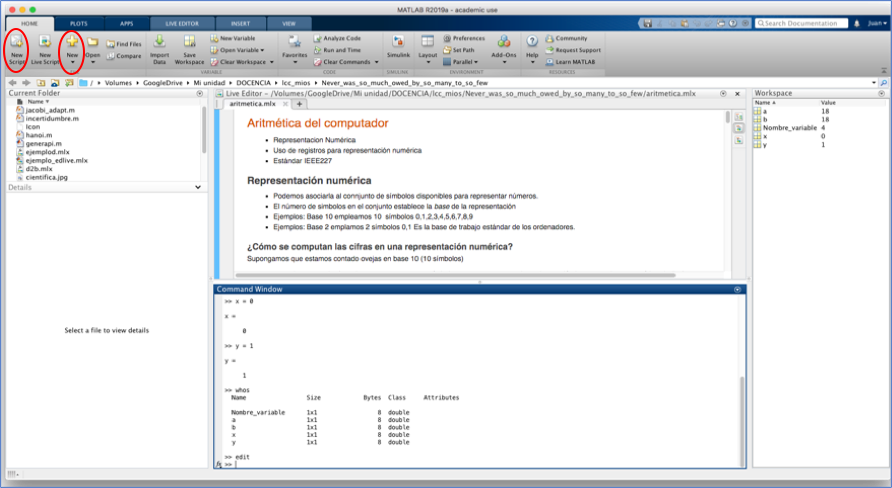
\includegraphics[width=14cm]{opened.png}
\caption{posición del botón  \emph{New Script} y del  menú \emph{New} en el IDE de Matlab (Señalados en rojo}.
\label{fig:opened}
\end{figure}

La otra opción es emplear el comando \texttt{edit}. Este comando puede emplearse de dos maneras. Si se escribe en la ventana de comandos,

\begin{verbatim}
>>edit
\end{verbatim}
Matlab abrirá el editor de textos y creará un documento nuevo sin nombre (\emph{untitled}.

Si añadimos a continuación del comando \texttt{edit} el nombre de un fichero,
\begin{verbatim}
>>edit ejemplo1.m
\end{verbatim}

Buscará un fichero con dicho nombre en los directorios de Matlab y en el directorio de trabajo. Si lo encuentra, abrirá el archivo encontrado. Si no lo encuentra, creará uno nuevo con dicho nombre. La figura \ref{fig:edv} muestra el editor de textos de Matlab ---Integrado en la parte central superior del IDE de Matlab--- con el contenido del fichero \texttt{ejemplo1.m}. Además, de entre las pestañas situadas en la parte superior del IDE, se ha seleccionado la marcada como \emph{EDITOR}. Es posible observar las barras de menú y de herramientas de las que dispone el editor de texto, para facilitar el trabajo de programación. 
\begin{figure}[h]
\centering
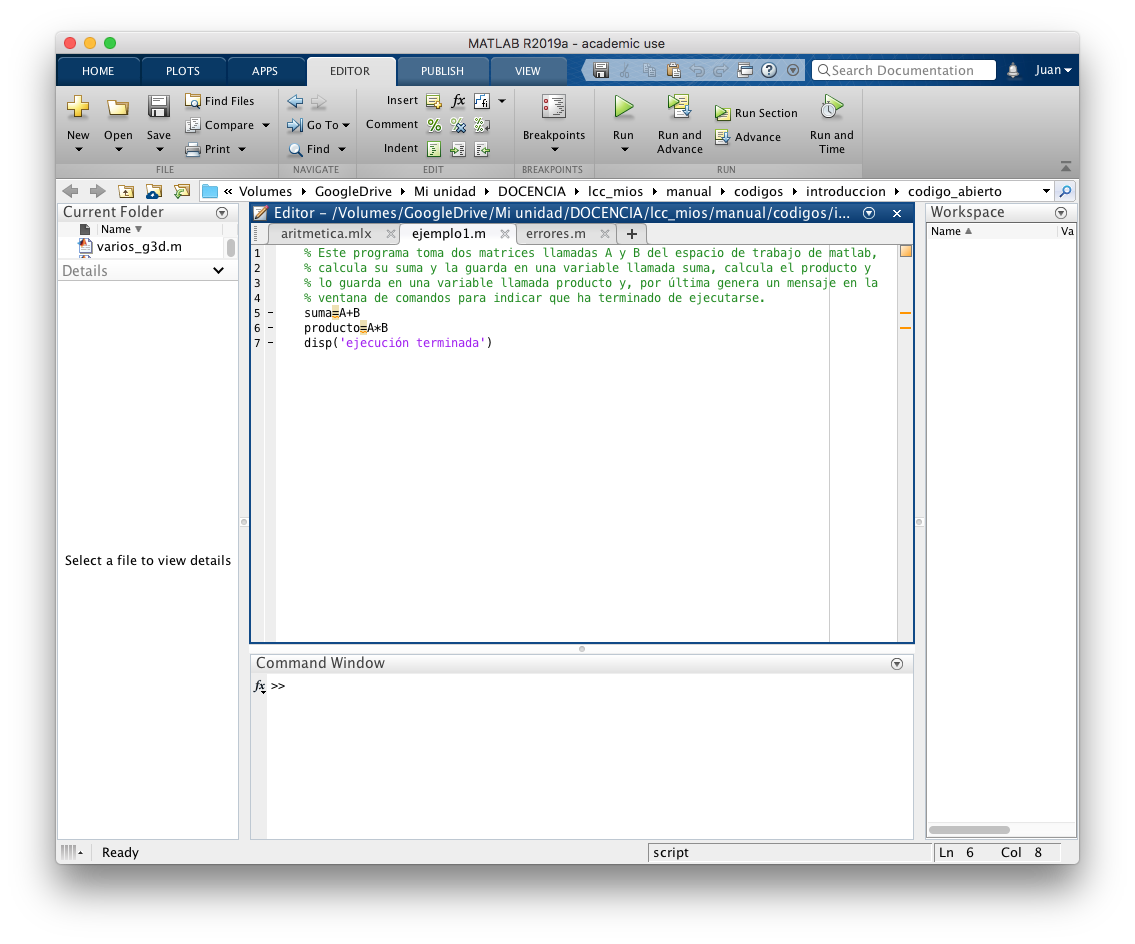
\includegraphics[width=14cm]{ejemplo1.png}
\caption{Vista del editor de textos de Matlab mostrando el contenido del fichero ejemplo1.m}
\label{fig:edv}
\end{figure}
Éstas, entre otras facilidades --resaltar texto de palabras clave, cotar número de líneas, sangrar estructuras de programación, etc.-- hacen que resulte especialmente atractivo emplear el editor de textos de Matlab en lugar de emplear otro editor de textos genérico.

\subsection{Scripts} \index{Script}
Un script en Matlab es un simple fichero de texto que contiene un conjunto de sentencias de Matlab válidas. La manera de ejecutarlo, consiste en escribir el nombre del fichero en la línea de comandos de Matlab. Matlab va leyendo el contenido del fichero línea a línea, y va ejecutando los comandos que contiene cada línea exactamente igual que si se hubieran escrito directamente en la línea de comandos de Matlab. Veamos un ejemplo sencillo, que corresponde con el código contenido en la figura \ref{fig:edv}:
%\begin{lstlisting}
% Este programa toma dos matrices llamadas A y B del espacio de trabajo de
%  Matlab, calcula su suma y la guarda en una variable llamada suma, calcula el 
% producto y lo guarda en una variable llamada producto y, por última genera un 
% mensaje en la ventana de comandos para indicar que ha terminado de ejecutarse.
%suma=A+B
%producto=A*B
%disp('ejecución terminada') 
%\end{lstlisting}
Si escribimos el texto anterior en un archivo y lo guardamos con el nombre ejemplo1.m, podemos ejecutar su contenido en Matlab sin más que escribir en la línea de comandos:
\begin{verbatim}
>> ejemplo1
\end{verbatim}

Las cuatro primeras líneas de código que empiezan con el símbolo \% no se ejecutan. Cuando Matlab encuentra una línea que empieza con dicho símbolo interpreta que se trata de un comentario escrito por el programador, para explicar qué hace el programa o aclarar algún aspecto de su funcionamiento. Cuando el editor de Matlab detecta el símbolo \% en una línea de código, resalta en color verde todo el texto de la línea a partir de dicho símbolo. De este modo, es inmediato ver que se trata de un comentario y que Matlab no tratará de ejecutarlo.

Un aspecto importante de la programación en Matlab, y en cualquier otro lenguaje de programación, lo constituye el comentario del código de programa; facilita su uso por otros usuarios y permite al programador recordar qué fue lo que hizo cuando lo programó. La experiencia demuestra que, en poco tiempo, los programas no comentados se vuelven incompresibles incluso para quien los escribió.

La quinta línea del programa busca en el \emph{workspace} las variables \texttt{A} y \texttt{B}. Si las variables no existen, es decir, si no han sido creadas previamente, el programa da un error, exactamente igual que si hubiéramos escrito directamente en la ventana de comandos de Matlab la sentencia \texttt{suma=A+B} sin haber definido antes \texttt{A} y \texttt{B}. Si las variables existen calcula la suma y guarda el resultado en el \emph{workspace} en la variable \texttt{suma}. La siguiente línea de código realiza el cálculo del producto de las dos variables y guarda el resultado en la variable \texttt{producto}. La última línea del programa mostrará en la ventana de comandos la frase,

\begin{verbatim}
ejecución terminada
\end{verbatim}
Para ello emplea la función de Matlab \texttt{disp} que escribe en la ventana de comandos cadenas de caracteres.

Un aspecto muy importante de los \emph{scripts} es que hacen uso del \emph{workspace} de Matlab tanto para buscar las variables que emplean como para guardar las variables resultantes de sus cálculo. Su ejecución es idéntica a la que se realizaría si copiáramos línea a línea en la ventana de comandos y las fuéramos ejecutando una detrás de otra.

\subsection{Funciones} \index{Funciones! Definición de funciones en matlab}
Las funciones juegan un papel fundamental en cualquier lenguaje de programación. En el caso de Matlab, se escriben como ficheros de texto, de modo análogo a los \emph{scripts}. lo que determina que Matlab los interprete como funciones es su primera línea de código.  Nos referiremos a esta primera línea con el nombre de \emph{cabecera de la función}. La cabecera de una función debe empezar siempre por la palabra clave \texttt{function}. Debe contener además, como mínimo, el nombre de la función. Por ejemplo,
\begin{verbatim}
function raices
\end{verbatim}

Un detalle importante en Matlab es que el fichero de texto que contiene la función debe llamarse igual que ésta, para que Matlab pueda identificar la función correctamente. Es decir, en el caso del ejemplo anterior, el fichero que contenga la función debe llamarse raíces.m.

A parte del nombre de la función la cabecera puede incluir también nombres de las variables de entrada. Estos se escriben a continuación del nombre de la función, separadas por comas y encerradas entre paréntesis,

\begin{verbatim}
function raices(a,b,c)
\end{verbatim}

En este ejemplo \texttt{a}, \texttt{b} y \texttt{c} son variables de entrada de la función \texttt{raices}. La razón por la que hay que incluir estas variables de entrada es que, a diferencia de los \emph{scripts}, las funciones no pueden acceder directamente a los valores de las variables contenidos en el \emph{workspace} de Matlab. Cuando se ejecuta una función es preciso dar valores a las variables que necesite utilizar, y que no se definan expresamente en el código de la función. Aclararemos esto más tarde con un ejemplo.

Por último la cabecera de una función puede incluir también una o varias variables de salida. Estas se escriben delante del nombre de la función separadas por comas y encerradas entre corchetes. Entre la(s) variable(s) de salida y el nombre de la función se incluye el símbolo de asignación \texttt{=}, para indicar que los resultados obtenidos por la función se han asignado (guardado en) a dichas variables.

\begin{verbatim}
function [x1,x2]=raices(a,b,c)
\end{verbatim}
  
En este caso, las variables de salida serían \texttt{x1} y \texttt{x2}.

A continuación, vamos a completar el ejemplo para el que hemos construido la cabecera en los párrafos anteriores. Se trata de una función que obtiene las raíces de una ecuación de segundo grado, $ax^2+bx+c=0$ conocidos sus coeficientes $a, b, c$,

%\lstinputlisting{../codigo/matlab/introduccion/raices.m}

Deberemos guardar estas líneas de código en un archivo con el nombre raices.m. Podemos ahora emplear la función \texttt(raices) para calcular las raíces de una ecuación de segundo grado. Supongamos que queremos obtener las raíces de la ecuación,
\begin{equation*}
x^2+x-6
\end{equation*}

si escribimos en la línea de comandos,
\begin{verbatim}
>>[raiz1, raiz2]=raices(1,1,-6)
\end{verbatim}
Matlab mostrará en la pantalla,

\begin{verbatim}
x1 =

     2
     
x2 =

    -3


raiz1 =

     2


raiz2 =

    -3

\end{verbatim}

Analicemos con un poco de detalle lo que hemos hecho. Al escribir: \texttt{[raiz1,raiz2] =} \texttt{raices (1,1,-6)}, hemos \emph{llamado} a la función \texttt{raices}, indicando que las variables de entrada deben tomar los valores \texttt{a=1},\texttt{b=1}, \texttt{c=-6}, es decir, los valores de los coeficientes de la ecuación de segundo grado cuya solución queremos obtener. Además hemos pedido a Matlab que guarde los resultados en el \emph{workspace} en las variable \texttt{raiz1} y \texttt{raiz2}. Cuando, tras llamar a la función, pulsamos el retorno de carro, Matlab empieza a ejecutar el código de la misma. Lo primero que hace es crear las variables \texttt{a}, \texttt{b} y \textbf{c} y asignarle los valores 1,1 y -6. Matlab crea estas variables pero no las guarda en el workspace sino en un espacio de memoria al que solo tiene acceso la función \texttt{raices}, desde la que se han creado. 
Esto constituye una característica muy importante de las funciones en Matlab. Cada vez que se llama a una función, se crea un espacio de memoria en la que se guardan las variable definidas en la función y a la que solo ésta tiene acceso. Además, una función no puede acceder ni modificar directamente ninguna variable que esté en el \emph{workspace}.

Una vez que la función ha asignado valores a las variable de entrada, comienza a realizar los cálculos pedidos, en primer lugar calcula la raíz correspondiente al discriminante positivo,
\begin{equation*}
+\sqrt{b^2-4ac}
\end{equation*}
y crea la variable \texttt{x1} para guardar el resultado. La variable \texttt{x1} solo existe en la memoria de la función \texttt{raices} y por tanto no existe ni es accesible desde el \emph{workspace}. Como no hemos terminado la línea de programa en la que se calcula \texttt{x1} con un punto y coma, Matlab muestra en la ventana de comandos el resultado del cálculo realizado. 

La raíz correspondiente al discriminante negativo se calcula de modo análogo. Una vez terminada la ejecución de la líneas del programa, Matlab vuelve a examinar la cabecera del programa y observa que debe dar como resultado, los valores contenidos en las variables \texttt{x1} y \texttt{x2}. Para ello, crea la variable \texttt{raiz1}  en el \emph{workspace} y copia en ella el contenido de la variable \texttt{x1}. Análogamente crea la variable \texttt{raiz2} y copia en ella el contenido de la variable \texttt{x2}. Con esto ha terminado la ejecución del programa. Matlab destruye las variables \texttt{x1} y \texttt{x2} que solo han existido durante la ejecución del programa, y nos muestra de nuevo el \emph{prompt} en la ventana de comandos para indicarnos que esta listo para ejecutar nuevas órdenes. Si analizamos el contenido del \emph{workspace}, empleando el comando \texttt{who} de Matlab,
\begin{verbatim}
>> who

Your variables are:

raiz1  raiz2  

\end{verbatim}
observaremos que allí están las variable \texttt{raiz1} y \texttt{raiz2}, que contienen las raíces de la ecuación de segundo grado que queríamos resolver.

En el ejemplo anterior hemos asignado directamente valores a las variables de entrada de la función \texttt{raices}. En Matlab, una función puede también asignar valores a sus variable de entrada copiándolos de los de otras variables existentes en el workspace, supongamos que creamos en el workspace de Matlab, tres variables con los valores de los coeficientes de la ecuación de segundo grado del ejemplo anterior,
\begin{verbatim}
>>coef1=1, coef2=1 coef3=-6
\end{verbatim}

Podríamos entonces llamar a nuestra función raíces, sustituyendo los valores de la variables de entrada por los nombres de éstas variables,

\begin{verbatim}
>> [raiz1, raiz2]= raices(coef1,coe2,coef3)
\end{verbatim} 
 Matlab, copiará ahora los valores contenidos en \texttt{coef1}, \texttt{coef2} y \texttt{coef3} en las variables de entrada de la función \texttt{a}, \texttt{b}, \texttt{c}. Ni que decir tiene, que el resultado final de la ejecución será el mismo.

\paragraph{Ámbito de una variable} \index{Variable! Ámbito de una variable}\index{Variable!Ámbito}La importancia del concepto de función está precisamente en el tratamiento que hace de las variables. Para entenderlo mejor, introduciremos el concepto de \emph{ámbito} de una variable.

Como hemos visto, la forma usual de crear una variable en Matlab es mediante el símbolo de asignación. Cuando asignamos un valor o el resultado de una operación a una variable en la ventana de comandos de Matlab,

\begin{verbatim}
>> a=18

a =

    18

\end{verbatim} 
 
Matlab reserva un espacio de memoria del computador para guardar la variable con el valor asignado. Esta variable forma parte del \emph{workspace} de Matlab, que constituye su ámbito propio. La variable creada es solo visible para aquellos comandos y sentencias que,
\begin{enumerate}
\item Se ejecutan desde la ventana de comandos de Matlab.
\item Se ejecutan desde un script.
\end{enumerate}

Cuando ejecutamos una función desde la ventana de comandos de Matlab, la función crea su propio espacio de memoria. Por así decir, es como un \emph{workspace} particular de la función. Cualquier variable que cree la función se guardará en el espacio de memoria de la función, que constituirá su ámbito propio. La variable creada dentro de la función solo es visible para aquellos comandos y sentencias que se ejecutan dentro de la función.

Una vez que termina la ejecución de una función, el espacio de memoria que se creó al ejecutarse se destruye y con él cualquier variable que el programa haya creado durante su ejecución.

La única manera de pasar información contenida en una variable del \emph{workspace} de Matlab a una función es copiándola a una variable de entrada de la función.

La única manera de pasar información contenida en una variable del espacio de memoria de una función, al workspace de Matlab, es copiándola a través de una variable de salida de la función.


\begin{figure}[h]
\centering
\begin{tikzpicture}
%\usetikzlibrary{shapes.multipart}
\path (5,0) node(a) [rectangle split,rectangle split parts =2,draw=blue,top color=white,bottom color=blue!15, very thick,align=left,rounded corners]{Ventana de comandos de Matlab
\nodepart{two}
\textgreater \textgreater a=3\\
\textgreater \textgreater b=2\\
\textgreater \textgreater y=ejem(a)\\
y =\\
    12\\
\textgreater \textgreater}		
(0,-7) node(b)[rectangle split,rectangle split parts =2,draw=blue, thick,rounded corners,align=left]{\emph{workspace de Matlab}\\
\nodepart{two}
a=3\\
b=2\\
...\\
tras ejecutar ejem\\
y=12
}
(10,-7) node(c)[rectangle split,rectangle split parts =2,draw=red,thick,rounded corners,align=left]{Espacio de memoria\\ de la funcion\\ \texttt{ejem.m}
\nodepart{two}
ent=3\\
b=4\\
sal=12\\
...\\
tras ejecutar ejem\\
se destruyen\\
todas las variables}
(5,-7) node(d)[rectangle,draw=red,top color=white, bottom color=red!15,align=left,very thick, rounded corners]{function sal=ejem(ent)\\ 
b=4;\\
sal=b*ent;}
(5,-5)node(e)[circle,draw=black,left color=blue!20,right color=red!20,thick,align=center]{Copiar\\ a en ent}
(5,-9)node(f)[circle,draw=black,left color=blue!20,right color=red!20,thick,align=center]{Copiar\\ sal en y};
\draw[blue,-latex](a.west)to [out=180, in=90]node[auto,swap]{Crea a y b} (b);
\draw[blue,-latex](a.south west)to [out=225, in=135]node[auto,align=center]{llamada a la\\ función\\ ejem($\cdot$)} (d.north west);
\draw[black,-latex](b.north east)to [out=45, in=180](e);
\draw[black,-latex](e.east)to [out=0, in=135](c.north west);
\draw[red,-latex](d.north)to [out=90, in=270](e);
\draw[black,-latex](c.south west)to [out=225, in=0](f);
\draw[black,-latex](f.west)to [out=180, in=315](b.south east);
\draw[red,-latex](d.south)to [out=270, in=90](f);
\draw[red,-latex](d.east)to node[auto,swap,align=center]{Crea b\\ y sal}(c);
\draw[red,-latex](d.north east)to [out=45, in=315]node[auto,align=center]{devolución\\ control\\ ventana de comandos} (a.south east);
\end{tikzpicture}
\caption{Ejemplo de uso de memoria y ámbito de variables durante la ejecución de una función}
\label{fig:amb}
\end{figure} 

La figura \ref{fig:amb} muestra esquemáticamente como se gestionan las variables en Matlab. En el cuadro superior se muestra la ejecución de varias sentencias en la ventana de trabajo de Matlab. Las dos primeras crean directamente dos variables \texttt{a} y \texttt{b} que se almacenan en el \emph{workspace de Matlab}, representado por el cuadro azul de la derecha. 
A continuación se llama a la función ejem (cuadro rojo central), asignándole como variable de entrada la variable \texttt{a} y como variable de salida la variable \texttt{y}. La ventana de comandos \emph{cede} el control a la función que empieza a ejecutarse:
\begin{enumerate}
\item La función crea su propio espacio de memoria (cuadro rojo de la izquierda)
\item Copia el valor contenido en la variable \texttt{a} en la variable \texttt{ent}. Esta variable se almacena en el espacio de memoria de la función.
\item Crea la variable \texttt{b} asignándole el valor 4 y la guarda en el espacio de memoria de la función. 

A partir de este momento y hasta el final de la ejecución de la función hay dos variables con el mismo nombre: \texttt{b=2} en el \emph{workspace} de Matlab; \texttt{b=4} en el espacio de memoria de la función. Las dos variables coexisten pero no se pueden confundir porque pertenecen a ámbitos distintos.
\item Crea la variable sal asignándole el producto de \texttt{b=4} por \texttt{ent=3}. Almacena la variable sal en el espacio de memoria de la función.
\item La función a llegado al final de su código. vuelve a leer la cabecera y crea la variable \texttt{y} en el workspace de Matlab, copiando el contenido de la variable \texttt{sal}.
\item termina la ejecución destruyendo el espacio de memoria de la función y \emph{devolviendo} el control a la ventana de comandos.
\end{enumerate}

\paragraph{Llamar a una función desde otra función.}
En Matlab, como en cualquier lenguaje de alto nivel, es posible llamar una función desde dentro de otra. Incluso es posible que una función se llame a sí misma, aunque este caso lo veremos más adelante cuando hablemos de control de flujo. 

Veamos un ejemplo sencillo de llamada de una función desde otra,

%\begin{lstlisting}
function salida=ejemplo2(entrada)
% esta funcion toma el valor de entrada lo eleva al cuadrado y pasa el
% resultado aun segunda función que calcula la raiz cuadrada...
% entrada y salida deberían ser iguales al final

%x=entrada^2;

%%%%    llamada a la segunda función%%%%
%salida=raiz(x);
%\end{lstlisting}

La función \texttt{ejemplo2} llama a una segunda función \texttt{raiz} cuyo código,

%\begin{lstlisting}
%function out=raiz(in)
%out=in^(1/2);
%\end{lstlisting}

Debe guardarse en uno de los tres lugares siguientes:
\begin{enumerate}
\item En el mismo fichero, ejemplo2.m en que se encuentra escrito el código de la función \texttt{ejemplo2}, justo debajo de dicha función.
\item En un fichero propio, raiz.m guardado en el directorio en que Matlab está trabajando.
\item En un fichero propio, raiz.m guardado en cualquier directorio de los incluidos en el \emph{path} de Matlab.
\end{enumerate}

Además al ejecutar la función \texttt{ejemplo2}, se buscará el código de la función raíz, precisamente en el orden que acabamos de indicar. Si añadimos directemente el código de la función \texttt{raiz} al fichero ejemplo2.m, el código quedaría,

%\begin{lstlisting}
%function salida=ejemplo2(entrada)
% esta funcion toma el valor de entrada lo eleva al cuadrado y pasa el
% resultado aun segunda función que calcula la raiz cuadrada...
% entrada y salida deberían ser iguales al final

%x=entrada^2;

%%%%    llamada a la segunda función%%%%
%salida=raiz(x);

%%%%%%    codigo de la segunda funcion%%%%%
%function out=raiz(in)
%disp('version incluida en el archivo ejemplo2.m')
%out=in^(1/2);
%\end{lstlisting}


La ventaja de escribir el código de la segunda función en el mismo fichero de la primera es que el acceso es más rápido. Sin embargo, solo la función \texttt{ejemplo2} podrá llamarla. Es decir la función \texttt{raiz} no puede emplearse desde la ventana de comandos de Matlab  ni desde ninguna otra función.

En general, si escribimos en un archivo .m de Matlab varias funciones,

% \begin{lstlisting}
% function a=uno(b)
% %aqui viene el codigo de la funcion uno
% ...

% function c=dos(d)
% % aqui viene el codigo de la funcion dos
% ...

% function e=tres(f)
% % aqui viene el codigo de la funcion dos
% ...
% .
% .
% .
% \end{lstlisting}

Todas las funciones incluidas en el fichero pueden llamarse entre unas a otras, pero solo la primera de ellas puede ser ejecutada desde la ventana de comandos de Matlab. Además el nombre del fichero debe coincidir con el nombre de la primera función  contenida en él. En el ejemplo que acabamos de esbozar, el fichero debería llamarse uno.m.

Evidentemente si cada función está guardada en un fichero .m distinto, todas las funciones pueden en principio ser ejecutadas desde otra función o desde la ventana de comandos de Matlab.

Cada vez que se ejecuta una función, ésta crea su propio espacio de memoria. Las variables incluidas en la cabecera de la función como variables de entrada y salida se copian, tal y como hemos visto para el caso de una función simple, entre el espacio de memoria propio de la función y el espacio de memoria de la función que la ha llamado.

  
\subsection{Funciones incluidas en Matlab.}\index{Funciónes! Funciones incluidas en matlab} 
Matlab incluye cientos de funciones. Estas funciones, están escritas con la misma filosofía que acabamos de describir aquí, es decir, admiten una o varias variables de entrada y devuelven sus resultados en una o varias funciones de salida. En algunos casos, se trata de ficheros de texto  guardados con la extensión \texttt{.m} iguales a los que nosotros podemos crear \footnote{En muchos casos las funciones incluidas en Matlab no están escritas en ficheros de texto accesibles para el usuario. Por razones de eficiencia, se trata de versiones de las funciones escritas por lo general en lenguaje C y compiladas.}. La manera de emplearlas desde la ventana de comandos de Matlab es idéntica a la descrita para las funciones creadas por el usuario. 

En la tabla \ref{tabfun}, se incluyen algunos ejemplos de las funciones matemáticas más corrientes. Son solo una pequeña muestra de las funciones disponibles. Para obtener una visión más completa de las funciones disponibles se aconseja emplear la ayuda de Matlab.

\begin{table}
\caption{Algunas funciones matemáticas en Matlab de uso frecuente}
\label{tabfun}
\begin{tabular}{c|c|c|c}
tipo&nombre&variables&función matemática\\
\hline
\hline
Trigonométrica&cos&y=cos(x)&coseno de un ángulo en radianes\\
\hline
Trigonométrica&sin&y=sin(x)&seno de un ángulo en radianes\\
\hline
Trigonométricas&tan&y=tan(x)&tangente de un ángulo en radianes\\
\hline
Trigonométricas&csc&y=csc(x)&cosecante de un ángulo en radianes\\
\hline
Trigonométricas&sec&y=sec(x)&secante de un ángulo en radianes\\
\hline
Trigonométricas&cot&y=cot(x)&cotangente de un ángulo en radianes\\

\hline
Trigonométricas&...&y=a...(x)&inversa de una función trigonométrica en radianes\\
&asin&y=asin(x)&ejemplo, arcoseno en radianes\\
\hline
\hline
Exponencial&exp&y=exp(x)&$e^x$\\
\hline
Exponencial&log&y=log(x)&logaritmo natural\\
\hline
Exponencial&log10&log10(x)&logaritmo en base 10\\
\hline
Exponecial&sqrt&y=sqrt(x)&$\sqrt(x)$\\
\hline
\hline
Redondeo&ceil&y=ceil(x)& redondeo hacia $+\infty$\\
\hline
Redondeo&floor&y=floor(x)&redondeo hacia $-\infty$\\
\hline
Redondeo&round&y=round(x)&redondeo al entero más próximo\\
\hline
Redondeo&fix&y=fix(x)&redondeo hacia $0$\\
\hline
Redondeo&rem&r=rem(x,y)&resto de la división entera de y entre x\\
\hline
\hline
Módulos&norm&y=norm(x)& módulo de un vector x\\
\hline
Módulos&abs&y=abs(x)&valor absoluto de x,(módulo de x si x es complejo)\\
\hline
Módulos&sign&y=sign(x)&función signo; 1 si x $>$ 0, -1 si x $<$ 0, 0 si x=0\\
\end{tabular}
\end{table}

\subsection{Depuración.}\index{Depurador}
Siempre que escribimos un programa, tanto si se trata de un \emph{script} como si es una función, es preciso comprobar su funcionamiento y, en  muchos casos corregir los errores cometido. El proceso de corrección de código desde su versión original hasta la versión definitiva se conoce con el nombre de depuración de código. Podemos distinguir dos tipos fundamentales de errores:

\begin{enumerate} 
\item Errores de sintaxis. \index{Error! De sintáxis}Normalmente son errores de escritura. Hemos escrito mal el nombre de una función o un comando o bien no hemos escrito correctamente el código siguiendo las reglas del lenguaje. Matlab advierte directamente de estos errores, cuando se trata de ejecutar el código, escribiendo en la ventana de comandos un mensaje de error. Como ejemplo veamos los errores del siguiente \texttt{script},

% \begin{lstlisting}
% % script con errores,
% y=[1 2 3; 4 5 6; 2 3] % a esta matriz le falta un elemento en la última fila

% x=[1 2 3; 4 5 6]
% z=y*x % las matrices no pueden multiplicarse entre si por que no coinciden
%       % numero de columnas de la primera con numero de filas de la segunda
% \end{lstlisting}

Si observamos el editor de textos, figura \ref{fig:ederror}, puede observarse algunas de los caracteres del texto subrayados en rojo. Esto puede indicar la existencia de errores en esa línea de código, como en el caso del carácter que se ha rodeado en la figura de un círculo rojo. 

En otros casos, --circulo azul de la figura-- se trata de advertencias, el programa funciona pero puede hacerlo de forma más eficiente; en el caso de la figura simplemente nos sugiere que añadamos un punto y coma al final de las sentencias, para que Matlab no escriba el resultado de cada cálculo en la ventana de comandos. No se trata por tanto de errores sino de advertir al programador que con puntos y comas su programa se ejecutará más rápido.

\begin{figure}[h]
\centering
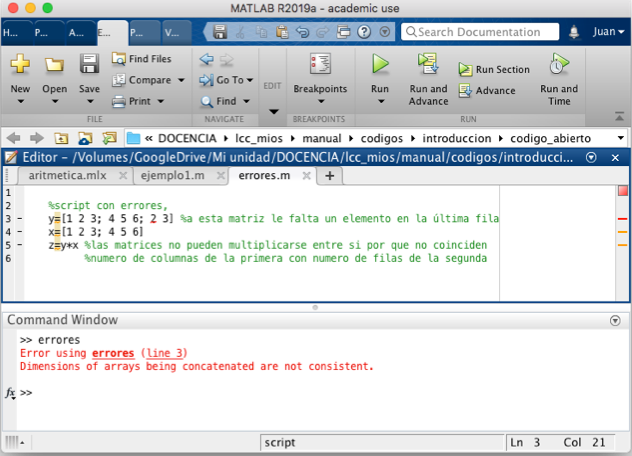
\includegraphics[width=14cm]{errores.png}
\caption{Vista de el editor de texto de Matlab. Circulo rojo error en el código. Rodeado en azul advertencias de posible mejoras. Rodeado en verde mensaje de error en tiempo de ejecución}
\label{fig:ederror}
\end{figure}

Si pasamos el ratón por encima de los caractéres en rojo, Matlab nos ofrece información adicional sobre el error detectado o la advertencia de mejora. La figura \ref{fig:popupm} muestra la información asociada al error rodeado en rojo en la figura anterior (ref{fig:ederror}).

\begin{figure}[h]
\centering
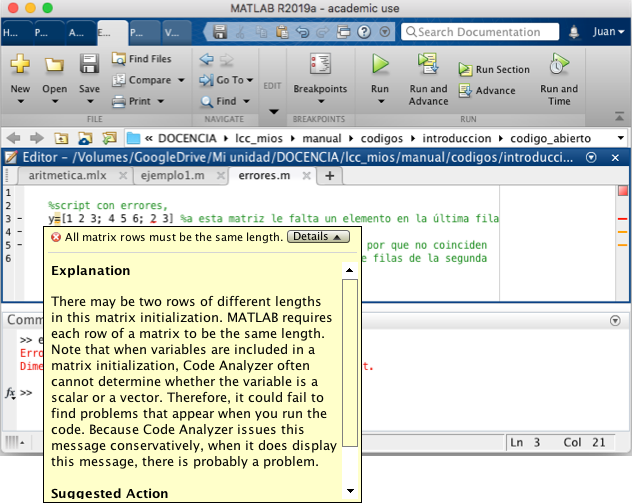
\includegraphics[width=14cm]{popupm.png}
\caption{Vista de el editor de texto de Matlab. Desplegable mostrando detalles sobre el error cometido}
\label{fig:popupm}
\end{figure}

Si ejecutamos el script, que hemos guardado con el nombre de \texttt{errores.m},

\begin{verbatim}
>> errores
Error using errores (line 3)
Dimensions of arrays being concatenated are not consistent.
\end{verbatim}

Matlab ha detectado el error en la construcción de la matriz \texttt{y}, nos indica mediante un mensaje el tipo de error cometido y la línea de código donde se ha producido y detiene la ejecución del \emph{script}. Se trata del mensaje rodeado en verde en la figura \ref{fig:ederror}.

Si corregimos el código, añadiendo a la matriz \texttt{y} el elemento que le falta,

% \begin{lstlisting}
% % script con errores,
% y=[1 2 3; 4 5 6; 2 3 8] % Ultima fila completada
% x=[1 2 3; 4 5 6]
% z=y*x % las matrices no pueden multiplicarse entre si por que no 
%       % coinciden numero de columnas de la primera con numero de
%       % filas de la segunda
% \end{lstlisting}
y volvemos a ejecutar el script.
\begin{verbatim}
>> errores

y =

     1     2     3
     4     5     6
     2     3     8


x =

     1     2     3
     4     5     6

Error using  * 
Incorrect dimensions for matrix multiplication. Check that the number of
columns in the first matrix matches the number of rows in the second matrix.
To perform elementwise multiplication, use '.*'.

Error in errores (line 5)
z=y*x % las matrices no pueden multiplicarse entre si por que no coinciden

\end{verbatim}
Matlab nos detecta el siguiente error cometido así como la línea en la que se comete. Es interesante notar que, aunque  se trata de un error de sistaxis, el editor de textos no puede detectarlo y, por tanto, no nos muestra ningún carácter subrrayado en rojo, asociado a él.

Si intercambiamos las posiciones entre las variables \texttt{x} e \texttt{y} en el producto, suponiendo que ésta es la causa del error cometido,

\begin{verbatim}
y=[1 2 3; 4 5 6; 2 3 8] 

x=[1 2 3; 4 5 6]
z=x*y 
\end{verbatim}

El código se ejecuta con normalidad,
\begin{verbatim}
>> errores

y =

     1     2     3
     4     5     6
     2     3     8


x =

     1     2     3
     4     5     6


z =

    15    21    39
    36    51    90
\end{verbatim}

\item Errores de codificación.\index{Errores! De codificación} Este segundo tipo de errores son mucho más difíciles de detectar. El código se ejecuta sin problemas, pero los resultados no son los esperados. Ante esta situación, no queda más remedio que ir revisando el código, paso a paso para detectar donde está el error.

El siguiente código del script \texttt{trect.m} muestra un error de este tipo, 

% \begin{lstlisting}
% % este script toma los valores de los catetos de un triángulo rectangulo del 
% % workspace de matlab (variables a y b). calcula su hipotenusa, y a partir
% % de estos datos, el seno el coseno y la tangente del angulo formado por la
% % hipotenusa y el cateto mayor que será siempre a

% % calculo hipotenusa,

% h=sqrt(a^2+b^2)

% % calculo del seno

% s=a/h

% % calculo del coseno
% a=b/h % error estamos sobreescribiendo el valor del coseno en la variable  
%       % que guardaba e valor del cateto

% % calculo de la tangente
% t=b/a

% \end{lstlisting}

%\lstinputlisting{../codigo/matlab/introduccion/trect.m}

El programa funciona perfectamente, por ejemplo si hacemos \texttt{a=4} y \texttt{b}=3,

\begin{verbatim}
>> trect

h =

     5


s =

    0.8000


a =

    0.6000


t =

     5
\end{verbatim}
Como hemos sobrescrito en \texttt{a} el valor del coseno, cuando tratamos de utilizar dicha variable como si fuera el cateto mayor para obtener la tangente, el resultado que obtenemos es erróneo.

El editor de texto de Matlab nos permite ejecutar un programa paso a paso, ver los valores que van tomando las variable en Matlab, etc, mediante el depurador que lleva incorporado. Para ello, se definen en el editor de Matlab \emph{breakpoints},esto es: líneas en las cuales Matlab detendrá la ejecución de un programa, entrará en modo de depuración y esperará instrucciones del usuario. La figura \ref{fig:depu1} muestra el código del ejemplo que acabamos de ver, en el que se ha definido un \texttt{breakpoint}, pulsando con el ratón sobre el guión que precede a la línea del programa en la que se desea parar la ejecución. Matlab indica que el \emph{breakpoint} está activo, cambiando el guión por un círculo rojo. Alternativamente, también es posible establecer o remover \emph{breackpoints} empleando el botón de la pestaña \emph{EDITOR}, rodeado de rojo en la figura.

\begin{figure}[h]
\centering
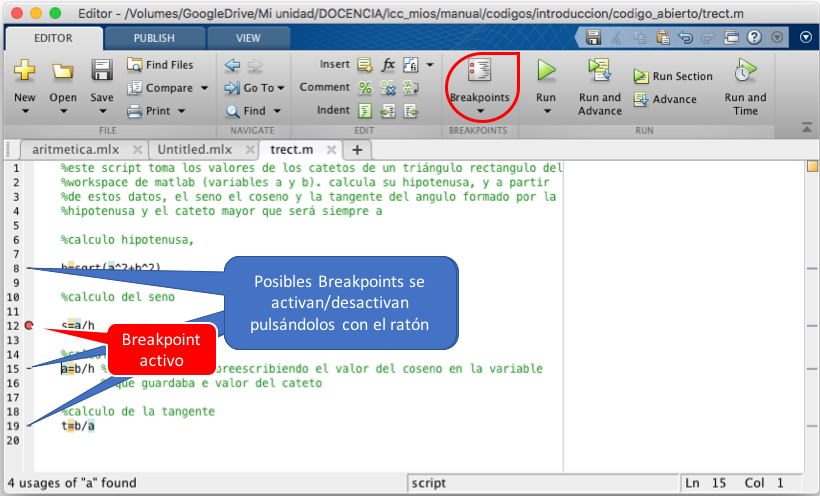
\includegraphics[width=14cm]{depu1.png}
\caption{Breakpoint activo}
\label{fig:depu1}
\end{figure}

Si una vez señalado el \emph{breakpoint}, ejecutamos el \emph{script},
\begin{verbatim}
>> trect

h =

    3.1477

12  s=a/h
K>> 
\end{verbatim}

Matlab nos indica que ha detenido la ejecución del programa en la línea marcada por el \emph{breakpoint} (línea 12 en el ejemplo). además vuelve a mostrar el \emph{prompt} en la ventana de comandos, pero esta vez precedido por la letra \texttt{k}, para indicarnos que ha entrado en modo de depuración.

A partir de aquí Matlab pone a nuestra disposición las herramientas de depuración, la figura \ref{fig:depu2} muestra la línea en que se ha parado la ejecución del programa, señalada con una flecha verde, y algunas de estas herraminentas. Básicamente nos da la posibilidad de ejecutar el código paso a paso, de entrar e ir paso a paso en las funciones que llama nuestro programa, o de de continuar la ejecución hasta que el final del programa o hasta el siguiente \emph{brakpoint} activo. Para dominar los detalles del depurador se aconseja leer la ayuda de Matlab.


\begin{figure}[h]
\centering
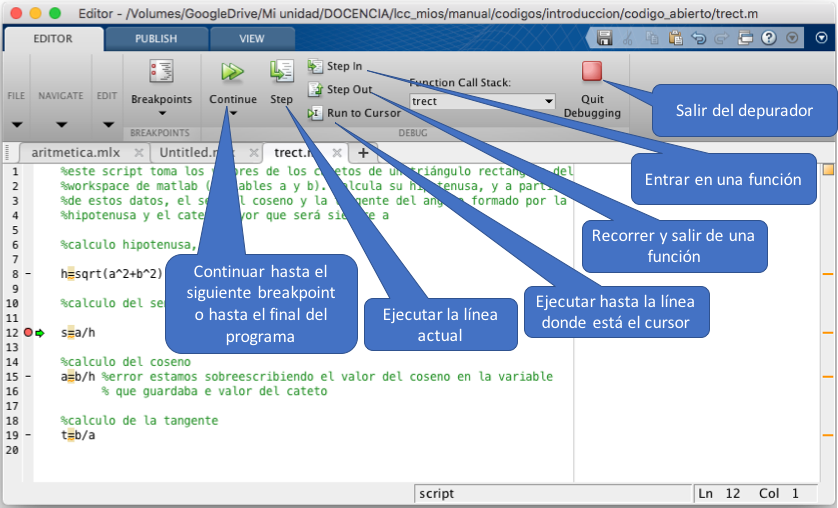
\includegraphics[width=14cm]{depu2.png}
\caption{Parada de programa en breakpoint y herramientas de depuración}
\label{fig:depu2}
\end{figure}

Si pulsamos el botón  "ejecutar línea actual" Matlab ejecutará la línea de programa señalada con la flecha verde y se parará en la línea siguiente. En cada paso, podemos ver el valor que toman las variables, pidiendo su valor directamente en la ventana de comandos,

\begin{verbatim}
K>> a

a =

    0.9531
\end{verbatim}

o bien señalando (sin pulsar botones) con el ratón en el editor de texto la variable de la que se trate.
En nuestro ejemplo del triángulo rectángulo es muy sencillo avanzar paso a paso en el programa con el depurador, y caer en la cuenta que, cuando se va a calcular la tangente, la variable \texttt{a} ya no contiene el valor del cateto.

\item Advertencias. \index{Advertencias} \index{Warnning}Por último señalar la existencia de los \emph{warnings} no se trata propiamente de errores, sino de simples advertencias de que algo puede funcionar de forma más eficiente, o puede no dar el resultado que esperábamos. En general, cuando se recibe un \emph{warning} al ejecutar un programa, o cuando el editor de Matlab subraya en rojo algún carácter en el editor de textos, se debe corregir el programa para que desaparezcan, aunque propiamente no se trate de errores.
\end{enumerate} 


 




\section{Control de Flujo}\index{Flujo} \index{Control de flujo}
En la sección anterior, se introdujo el modo de escribir programas en Matlab mediante el uso de 	\emph{scripts} y funciones. En todos los casos vistos, la ejecución del programa empezaba por la primera línea del programa, y continuaba, por orden, línea tras línea hasta alcanzar el final del programa. Se trata de programas en los que el \emph{flujo} es lineal, porque los resultados de cada línea de programa se van obteniendo regularmente uno detrás de otro. 

Hay ocasiones en las que, por diferentes razones que expondremos a continuación, puede interesarnos alterar el orden en que se ejecutan las sentencias de un programa, bien repitiendo una parte de los cálculos un determinado número de veces o bien ejecutando unas partes de código u otras en función de que se satisfagan unas determinadas condiciones.

El control del orden en que se ejecutan las sentencias de un programa es lo que se conoce con el nombre de \emph{control de flujo}. Veremos dos tipos principales de control de flujo: El flujo condicional y los bucles.
\subsection{Flujo condicional.}\index{Flujo!Condicional}
Empezaremos con un ejemplo sencillo de cómo y para qué condicionar el flujo de un programa. Supongamos que queremos construir un programa que reciba como variable de entrada un número cualquiera y nos muestra un mensaje por pantalla si el número es par.

Para ello, podríamos hacer uso de la función \texttt{rem} (ver tabla \ref{tabfun}). Si el resto de la división entre dos del número suministrado a la función es cero, se trata de un número par; si no, es un número impar. Podríamos hacer uso de operadores relacionales, en particular de \texttt{==} para comprobar si el resto de la división entre dos es cero. Por último necesitaríamos algún mecanismo que permitiera al programa escribir un mensaje solo cuando el número introducido sea par.

\paragraph{if - elseif - else - end.} El mecanismo que necesitamos nos lo suministra la estructura \texttt{if} de Matlab. Veamos en primer lugar el código del ejemplo del que venimos hablando,

% \begin{lstlisting}
% function espar(x)
% % Este programa recibe un numero entero como variable de entrada. y muestra
% % por pantalla un mensaje indicando si el numero recibido es par o impar.

% % Calculamos el resto de la division por dos
% resto=rem(x,2);

% % Empleamos una estructura if - else -end para decidir que mensaje mostrar

% if resto==0
%     % si el resto es cero el número es par
%     disp('el número es par')
% end
% \end{lstlisting}

El programa toma un número como variable de entrada y calcula el resto de su división entre dos. A continuación entra en una parte de código especial, que se inicia con la palabra clave \texttt{if} y termina con la palabra clave \texttt{end}. 

La palabra clave \texttt{if} va siempre seguida de una expresión que da un resultado lógico: verdadero ($1$) o falso ($0$). Esta expresión puede ser cualquier combinación válida de expresiones relacionales o lógicas. Esta expresión lógica, que sigue al if constituye una condición. El programa seguirá ejecutando las siguientes líneas solo si la condición se cumple; si no, se las saltará hasta llegar a la expresión \texttt{end}.

En nuestro ejemplo, se emplea una expresión relacional sencilla \texttt{resto==0}. Si se cumple, el programa ejecutará la siguiente línea de programa, escribiendo en la ventana de comandos la frase ``el número es par"  si no se cumple el programa se la salta, llega hasta el \texttt{end}, y no escribe nada por pantalla. 

Acabamos de ver la estructura condicional \texttt{if} más sencilla posible. Podríamos complicarla un poco pidiendo que también nos saque un mensaje por pantalla cuando el número sea impar. Esto supone incluir en nuestro programa una disyuntiva; si es par el programa debe hacer una cosa y si no, debe hacer otra. Para incluir este tipo de disyuntivas en una estructura \texttt{if}, se emplea la palabra clave \texttt{else}. Veamos nuestro ejemplo modificado,
% \begin{lstlisting}
% function espar(x)
% % Este programa recibe un numero entero como variable de entrada. y muestra
% % por pantalla un mensaje indicando si el numero recibido es par o impar.

% % Calculamos el resto de la division por dos
% resto=rem(x,2);

% % Empleamos una estructura if - else -end para decidir que mensaje mostrar

% if resto==0
%     % si el resto es cero el número es par
%     disp('el número es par')
% else
%     % si el resto no es cero el número es impar
%     disp('el número es impar')
% end 
% \end{lstlisting}

La palabra clave \texttt{else} marca ahora la disyuntiva, si el número es par, el programa ejecuta las líneas de código entre el \texttt{if} y el \texttt{else}, si el número no es par ejecutará las líneas entre el \texttt{else} y el \texttt{end}.

La estructura \texttt{if} admite todavía ampliar el número de posibilidades de elección mediante la palabra clave \texttt{elseif}. Al igual que  con \texttt{if}, \texttt{elseif} va seguido de una expresión lógica que establece una condición, si se cumple se ejecutará el código de las líneas siguientes, si no se cumple, el programa saltará a la siguiente línea que contenga una palabra clave: otro \texttt{elseif}, un \texttt{else} o directamente el \texttt{end} que marca el final de la parte de código condicional. Para ver cómo funciona, vamos a modificar nuestro ejemplo anterior, para que, si el número introducido no es divisible por dos, compruebe si es divisible por tres,

% \begin{lstlisting}
% function divis(x)
% % Este programa recibe un numero entero como variable de entrada. y muestra
% % por pantalla un mensaje indicando si el numero recibido es par. Si no 
% % es par, comprueba si es divisible por 3 y si lo es muestra un mensaje   
% % por pantalla indicandolo. Si no es par ni divisible por tres muestra un
% % mensaje diciendo que no es par ni disible por tres. 



% % Empleamos una estructura if-elseif-else-end para decidir que mensaje mostrar

% if rem(x,2)==0
%     % si el resto es cero el número es par
%     disp('el número es par')
% elseif rem(x,3)==0
%     % El número es divisible por tres
%     disp('el número es divisible por 3')
% else
%     % el numero no es par ni divisible por tres
%     disp('el número no es par ni divisible por 3')
% end
% \end{lstlisting}

Si llamamos ahora a la función dando como valor de entrada un número par, Ejecutará el código situado debajo del \texttt{if} y antes del \texttt{elseif} y se saltará todo lo demás hasta llegar al \texttt{end}. Si el número introducido no es par, pero es divisible por tres, se saltará el código situado por debajo del \texttt{if}, ejecutará el código contenido debajo del \texttt{elseif} hasta el \texttt{else} y saltará el resto del código hasta llegar al \texttt{end}. Por último si el número no es par ni divisible por tres, solo ejecutará el código situado por debajo del \texttt{else}.

Un aspecto que debemos resaltar, es que el programa ejecutará el código correspondiente a la primera condición que se cumpla, y se saltará el resto hasta llegar al \texttt{end}. Así por ejemplo, si en nuestro ejemplo introducimos el número $6$, el programa nos mostrará el mensaje ``el número es par", puesto que ésta es la primera condición que se cumple, pero nunca nos mostrará el mensaje ``el número es divisible por 3". Porque una vez comprobada y cumplida la primera condición (ser par) el programa salta directamente al \texttt{end} final de la estructura, sin comprobar nada más. La figura \ref{fig:if} muestra el esquema completo de una estructura \texttt{if}. Los términos entre paréntesis pueden estar o no presentes en una implementación concreta.

\begin{figure}[h]
\centering
\begin{tikzpicture}
%\usetikzlibrary{shapes.multipart}
\path (5,0) node(a) [rectangle split,rectangle split parts =2,draw=blue,top color=white,bottom color=blue!15, very thick,align=left,rounded corners]{Estructura if-elseif-else-end
\nodepart{two}

if condición\\
\ \ \ ... código\\
\ \ \ ...\\
(elseif condición)\\
\ \ \ ... código\\
\ \ \ ...\\
(elseif condición)\\
\ \ \ ... código\\
\ \ \ ...\\
.\\
(puede haber tantos bloques elseif como se necesiten)\\
.\\
(else)\\
\ \ \ ... código\\
\ \ \ ...\\
end};		
\end{tikzpicture}
\caption{Esquema general de la estructura de flujo condicional \texttt{if} los términos escritos entre paréntesis son opcionales.}
\label{fig:if}
\end{figure} 

\paragraph{Estructuras if anidadas.}\index{Anidación! If anidado} 
En el ejemplo anterior, hemos visto cómo, si el número introducido en la función era par y además divisible por tres, el programa nunca nos informaría de esta segunda propiedad, debido al carácter excluyente de la estructura \emph{if}. Una manera de resolver este problema, es mediante el uso de estructuras \texttt{if} anidadas. La idea es muy sencilla, se construye una estructura \texttt{if} para comprobar una determinada condición, si esta se cumple, dentro de su código se construye otra estructura if para comprobar una segunda condición, y así sucesivamente, todas las veces que sea necesario. Si modificamos nuestro ejemplo anterior, incluyendo un \texttt{if} anidado,

% \begin{lstlisting}
% function divis23(x)
% % Este programa recibe un numero entero como variable de entrada. y 
% % muestra por pantalla un mensaje indicando si el numero recibido es par. 
% % si el numero es par y divisible entre tres,
% % si es divisible entre tres  
% % Si no es par ni divisible por tres 



% % Empleamos una estructura if - else -end 
% % y un if anidado para decidir que mensaje mostrar

% if rem(x,2)==0
%     % si el resto es cero el número es par
%     % comprobamos con un if anidado si además es divisible entre tres
%     if rem(x,3)==0
%         disp('el número es par y divisible entre tres')
%     else
%         disp('el número es par')
%     end
% elseif rem(x,3)==0
%     % El número es divisble entre tres
%     disp('el número es divisible entre 3')
% else
%     % el numero no es par ni divisible entre tres
%     disp('el número no es par ni divisible entre tres')
% end
% \end{lstlisting}

\paragraph{Switch-case-otherwise.} \index{Flujo! Switch-case}Se trata de otra estructura que permite también ejecutar una parte u otra de código de acuerdo con unas codiciones preestablecida. Estas condiciones se presentan en forma de \emph{casos}, el programa comprueba al llegar a la estructura \texttt{switch} de qué caso se trata y ejecuta el código correspondiente. La figura \ref{fig:switch} muestra la forma general que toma una estructura \texttt{switch}.

La estructura \texttt{switch}, compara el valor contenido en la variable de entrada a la estructura con las expresiones contenidas en los casos, ejecutando el primer caso para el que coincidan. Si no encuentra ninguno, ejecuta entonces el código contenido debajo de la sentencia \texttt{otherwise}.

Veamos un ejemplo muy sencillo,

% \begin{lstlisting}
% function signo(x)
% % este programa emplea una estructura switch para informarnos del signo de
% % un número.

% % NOTA EL PROGRAMA NO COMPRUEBA QUE LA VARIABLE DE ENTRADA X SEA UN NUMERO,
% % SI ES UN VECTOR O UNA MATRIZ EL RESULTADO NO TIENE SENTIDO
  
% s=sign(x); % obtnemos el signo del número mediante la función sign

% % construimos la estructura switch,

% switch s
%     case 1
%         disp('el número es positivo')
%     case -1
%         disp('el número es negativo')
%     otherwise
%         disp('el número es cero')
% end

% \end{lstlisting}

\begin{figure}[h]
\centering
\begin{tikzpicture}
%\usetikzlibrary{shapes.multipart}
\path (5,0) node(a) [rectangle split,rectangle split parts =2,draw=green,top color=white,bottom color=green!20, very thick,align=left,rounded corners]{Estructura switch-case-otherwise
\nodepart{two}
switch variable\\
\ \ \ case expresión\\
\ \ \ \ \ ... código\\
\ \ \ case expresión\\
\ \ \ \ \ ... código\\
\ \ \ .\\
Puede haber tantos bloques \emph{case} como se necesiten\\
\ \ \ .\\
\ \ \ otherwise\\
\ \ \ \ \ ... código\\
end};		
\end{tikzpicture}
\caption{Esquema general de la estructura switch-case-otherwise}
\label{fig:switch}
\end{figure}

La función del ejemplo emplea a su vez la función de Matlab \texttt{sign} para obtener el signo ($1$, $-1$, $0$) del número introducido. Guarda el resultado de esta operación en la variable \texttt{s}, que será precisamente la variable de entrada a la estructura \texttt{switch}. Los casos se limitan a chequear los posibles valores de la variable y enviar a la ventana de comandos el mensaje correspondiente.
 
\subsection{Bucles}\index{Flujo!Bucles}\index{Bucles}
En ocasiones, es preciso repetir una operación un número determinado de veces o hasta que se cumple una cierta condición. Los lenguajes de alto nivel poseen estructuras específicas, para repetir la ejecución de un trozo de programa las veces que sea necesario. Cada repetición recibe el nombre de iteración. Estas estructuras reciben el nombre genérico de bucles. Vamos a ver dos tipos: los bucles \texttt{for} y los bucles \texttt{while}.

\paragraph{Bucles for.} \index{Flujo! Bucle for}\index{Bucles! Bucle for}Un bucle \texttt{for} repite las sentencias contenidas en el bucle un determinado número de veces, es decir realiza un número fijo de iteraciones. La estructura general de un bucle \texttt{for} se muestra en la figura, \ref{fig:for}

\begin{figure}[h]
\centering
\begin{tikzpicture}
%\usetikzlibrary{shapes.multipart}
\path (5,0) node(a) [rectangle split,rectangle split parts =2,draw=orange,top color=white,bottom color=orange!30, very thick,align=left,rounded corners]{Estructura de un bucle for
\nodepart{two}

for indice=[vector de valores]\\
\ \ \ ... código\\
(condición: Break)\\
\ \ \ ...\\
(condicición: Continue)\\
\ \ \ ... código\\

end};		
\end{tikzpicture}
\caption{Esquema general de la estructura de un bucle \texttt{for} los términos escritos entre paréntesis son opcionales.}
\label{fig:for}
\end{figure} 
 
El bucle empieza con la palabra clave for, seguida de una variable a la que hemos dado el nombre genérico de índice. Esta variable irá tomando sucesivamente los valores de los elementos contenidos en el [vector de valores]. El código contenido en el bucle, desde la línea siguiente al \texttt{for} hasta el \texttt{end} se ejecutará tantas veces como valores tenga el vector de valores. Antes de hablar de las sentencias \texttt{break} y \texttt{continue}, veamos alguno ejemplos.
% \begin{lstlisting}
% function y=demofor(x)
% % este programa emplea un bucle for sencillo para ir mostrando uno 
% % a uno los elementos del vector de entrada x por pantalla. además  
% % los suma y guarda el resultado total en el vector y,

% y=0; % iniciamos la suma a cero

% for i=x
%     disp(i)
%     y=y+i;
% end
% \end{lstlisting}

Si ejecutamos el programa, usando como entrada el vector \texttt{d=[1 9 4 18]},

\begin{verbatim}
>> d=[1 9 4 18]

d =

     1     9     4    18

>> suma=demofor(d)
     1

     9

     4

    18


suma =

    32
\end{verbatim}

Una vez que el programa llega al bucle \texttt{for}, iguala la variable \texttt{i} al primer valor contenido en el vector de entrada, lo muestra por pantalla y añade su valor a la variable de salida. cuando llega al \texttt{end} del bucle for comprueba que todavía quedan valores del vector de entrada por recorrer, así que vuelve al principio del \texttt{for}, igual la variable \texttt{i} al segundo valor del vector de entrada, suma dicho valor a la variable de salida, llega al \texttt{end} y así sucesivamente hasta que haya recorrido todos los valores del vector de entrada.

El uso más habitual de los bucles, es para recorrer elementos de un vector o de una matriz. por esta razón, lo más frecuente es que no se de explícitamente el vector cuyos elementos debe recorrer el índice del \texttt{for}, sino que se construya empleado el operador \texttt{:},
\begin{verbatim}
for indice=principio:incremento:final
\end{verbatim}

Veamos un ejemplo sencillo para obtener el vector suma de dos vectores,
% \begin{lstlisting}
% function s=sumafor(x,y)
% % este programa emplea un bucle for sencillo para sumar dos vectores
% % primero comprueba si son del mismo tamaño. Si no lo son da un mensaje 
% % de aviso

% l1=length(x);
% l2=length(y);
% if l1==l2
%     % construimos un vector de ceros del mismo tamaño que x e y paraa
%     % guardar el resultado de la suma,
%     s=zeros(size(x));
%     % si son iguales los suma elemento a elemento usando un bucle for
%     for i=1:l1
%         s(i)=x(i)+y(i);
%     end
% else
%     disp('los vectores son de distinto tamaño')
% end
% \end{lstlisting}

En la figura \ref{fig:for}, aparecen dos sentencias opcionales, \texttt{break} y \texttt{continue}.

La sentencia \texttt{break}, permite terminar el bucle \texttt{for} antes de que haya terminado de realizar todas las ejecuciones previstas. La sentencia break va siempre incluida dentro de una condición que, si se cumple interrumpe la ejecución del bucle. Por ejemplo, podemos emplear un bucle \texttt{for} y una sentencia \texttt{break}, para buscar la primera vez que un determinado número aparece en un vector,

% \begin{lstlisting}
% function posicion=buscanum(x,n)
% % este programa emplea un bucle for y un break para buscar en el  
% % vector x, la primera vez que aparece el número n

% % obtenemos la longitud del vector
% l1=length(x);
% % iniciamos la variable posicion a un valor absurdo
% posicion=-1;
% for i=1:l1
%     if x(i)==n
%         posicion=i:
%         break
%     end
% end
% if posicion==-1
%     disp('el numero pedido no se encuentra en el vector x') 
% end
% \end{lstlisting} 

El programa toma como variables de entrada un vector y el número que debe buscar dentro del vector. Construye un bucle \texttt{for}, con el mismo número de iteraciones que el tamaño del vector. El bucle va comparando los elementos del vector con el número pedido. Cuando encuentra un elemento igual, se ejecuta el código de la estructura if contenida en el bucle; la variable posición toma el valor del índice \texttt{i} del bucle y la sentencia \texttt{break} interrumpe la ejecución del bucle, saltando al final del mismo. Por último, se ha añadido una condición al terminar el bucle, para el caso de que se hayan recorrido todos los elementos del vector sin encontrar el número pedido.

La sentencia \texttt{continue}, se emplea para hacer que una determinada iteración interrumpa su ejecución y salte directamente al comienzo de la siguiente iteración. Debe ir, como en el caso de la sentencia \texttt{break}, incluida en una estructura condicional. Veamos un ejemplo para entender como funciona. Se trata de un programa que admite como entrada un vector de cualquier longitud y devuelve como salida otro vector que contiene solo los números pares contenidos en el vector de entrada,

% \begin{lstlisting}
% function pares=buscapar(x)
% % este programa emplea un bucle for y un continue para construir un 
% % vector de salida con los numeros pares contenidos en el vector de entrada.

% % obtenemos la longitud del vector
% l1=length(x);
% % iniciamos el vector de salida a un vector vacío,
% pares=[];
% for i=1:l1
%     if rem(x(i),2)~=0
%         continue
%     end
%     pares=[pares x(i)];
% end
% \end{lstlisting}

El funcionamiento es muy sencillo, en cada iteración la sentencia \texttt{if} comprueba si el número es par. Si no lo es, entra en el código de la estructura \texttt{if}, ejecuta la sentencia \texttt{continue}, y se salta el resto del código del bucle, volviendo directamente a empezar la siguiente iteración.

\paragraph{bucles for anidados.} \index{Anidación!For anidado}Los bucles \texttt{for} pueden anidarse unos dentro de otros de modo análogo a como se hace con las estructuras \texttt{if}. Veamos un ejemplo de uso, muy común; calcular la suma de dos matrices,

% \begin{lstlisting}
% function s=suma_mat(x,y)
% % este programa emplea dos bucles for anidados para obtener la suma de 
% % dos matrices.

% % obtenemos el tamaño de las matrices,
% t1=size(x);
% t2=size(y);
% if t1(1)==t2(1)&& t1(2)==t2(2)
%     % si las matrices tienen el mismo tamaño pueden sumarse...
%     % construimos una matriz de dicho tamaño para guardar el 
%     % resultado de la suma
%     s=zeros(size(x));
%     % construimos un bucle que recorre las filas de ambas matrices
%     for i=1:t1(1)
%         % y dentro, anidamos un bucle que recorre las columnas
%         for j=1:t1(2)
%             % Empleando ambos índices para ir sumando los elementos 
%             % de las dos matrices,
%             s(i,j)=x(i,j)+y(i,j);
%         end
%     end
% else
%     % si no tienen el mismo tamaño no se pueden sumar...
%     disp('las matrices no son del mismo tamaño')
% end
% \end{lstlisting} 

Es interesante observar en este ejemplo el funcionamiento de los dos bucles anidados. Cada interación del bucle exterior, avanza una fila, en el recorrido de las matrices, cada iteración del bucle interior recorre todos los elementos de la fila indicada por el bucle exterior.

\paragraph{bucle while.} \index{Flujo! Bucle while}\index{Bucles! Bucle while} Este bucle tiene la misma finalidad que un bucle \texttt{for}, repetir un trozo de código un determinado número de veces. Lo que cambia, es el mecanismo que determina cuantas iteraciones realizará el bucle. En el caso de un bucle \texttt{while} las iteraciones se repiten un número indefinido de veces mientras se cumpla una determinada condición impuesta al principio del bucle. La figura \ref{fig:while} muestra la estructura general de un bucle while.

\begin{figure}[h]
\centering
\begin{tikzpicture}
%\usetikzlibrary{shapes.multipart}
\path (5,0) node(a) [rectangle split,rectangle split parts =2,draw=yellow,top color=white,bottom color=yellow!40, very thick,align=left,rounded corners]{Estructura de un bucle while
\nodepart{two}

while condición\\
\ \ \ ... código\\
(condición: Break)\\
\ \ \ ...\\
(condicición: Continue)\\
\ \ \ ... código\\
end};		
\end{tikzpicture}
\caption{Esquema general de la estructura de un bucle \texttt{while} los términos escritos entre paréntesis son opcionales.}
\label{fig:while}
\end{figure}

Veamos un ejemplo sencillo. 

% \begin{lstlisting}
% function n=potencia(x,max)
% % este programa emplea un bucle while para calcular la potencia a 
% % la que hay que elevar un número x para que el resultado sea mayor 
% % que otro determinado número max
% % un número.

% % NOTA EL PROGRAMA NO COMPRUEBA QUE LA VARIABLE DE ENTRADA X SEA UN NUMERO,
% % Si ES UN VECTOR O UNA MATRIZ EL RESULTADO NO TIENE SENTIDO
  
% pot=1;
% n=0;
% while pot<max % mientras la potencia calculada sea menor que max
%     n=n+1;
%     pot=x^n;
% end
% \end{lstlisting}

El programa emplea un bucle \texttt{while} para calcular el exponente mínimo al que hay que elevar un número para que rebase una determinada cantidad. El bucle while se ejecuta mientras la potencia calculada sea menor que la variable \texttt{max}; una vez que la potencia rebasa dicho valor el bucle deja de ejecutarse. Un aspecto muy importante del bucle \texttt{while} es que al programarlo hay que asegurarse de que dentro del bucle existe la posibilidad de cambiar la condición de entrada. Si no, el programa no podrá terminar nunca el bucle\footnote{Cuando se produce esta situación por un error en el diseño del programa, el bucle se puede parar pulsando a la vez las teclas ctrl+c}.

Las sentencias \texttt{break} y \texttt{continue} son idénticas a las descritas en el caso de los bucles \texttt{for}, por lo que no insistiremos más sobre el asunto.

\paragraph{Bucles while anidados.} \index{Anidación! While anidado} Del mismo modo que se anidan los bucles \texttt{for}, es posible anidar bucles \texttt{while}. Como un ejemplo, vamos a reproducir el programa desarrollado antes para sumar dos matrices, empleando ahora bucles \texttt{while}.

% \begin{lstlisting}
% function s=suma_while(x,y)
% % este programa emplea dos bucles while anidados para obtener la 
% % suma de dos matrices.

% % obtenemos el tamaño de las matrices,
% t1=size(x);
% t2=size(y);
% if t1(1)==t2(1)&& t1(2)==t2(2)
%     % si las matrices tienen el mismo tamaño pueden sumarse...
%     % construimos una matriz de dicho tamaño para guardar el 
%     % resultado de la suma
%     s=zeros(size(x));
%     % construimos un bucle que recorre las filas de ambas matrices
%     i=1; % inicimos un contador para las filas
%     while i<=t1(1)
%         % y dentro, anidamos un bucle que recorre las columnas
%         j=1; % iniciamos un contador para las columnas
%         while j<=t1(2)
%             % Empleando ambos índices para ir sumando los elementos 
%             % de las dos matrices,
%             s(i,j)=x(i,j)+y(i,j);
%             j=j+1; % vamos incrementando el indice de columnas
%         end
%         i=i+1; % vamos incrementando el indice de filas
%     end
% else
%     % si no tienen el mismo tamaño no se pueden sumar...
%     disp('las matrices no son del mismo tamaño')
% end
% \end{lstlisting}

El ejemplo, es más complicado de programar y menos eficiente que si usáramos bucles \texttt{for}. La razón de incluirlo es puramente ilustrativa. En general, un bucle \texttt{while} debe utilizarse solo cuando el número de iteraciones que se precisa realizar no es fijo, sino que depende de alguna condición propia de los resultados que se van obteniendo a medida que se van realizando iteraciones.

\subsection{Funciones recursivas.} \index{Funciones! Recursivas}
Una función recursiva es una función que se llama a sí misma. Hemos esperado hasta aquí para hablar de ellas porque, de alguna manera, se comportan como un bucle y necesitan una condición de salida para dejar de llamarse a sí mismas y terminar su ejecución. En general, son delicadas de manejar y tienden a consumir mucha memoria ya que cada vez que la función se llama a sí misma necesita crear un nuevo espacio de memoria independiente. Veamos un ejemplo de función recurrente que permite obtener el término enésimo de la sucesión de Fibonacci  
\begin{align*}
f_0=0, f_1=1, f_2=1, f_3=2, f_4=3, f_5=5, f_6=8, \cdots f_i=f_{i-1}+f_{i-2} \cdots 
\end{align*}

La sucesión empieza con los términos $0$ y $1$ y a partir de ahí cada término es la suma de los dos anteriores. Podemos convertir directamente esta definición en código,

%\lstinputlisting{../codigo/matlab/introduccion/fibonacci.m}

Si n es menor que dos, la función da como valor el término correspondiente (1 o 0). Si n es mayor que dos, vuelve a llamarse a si misma con entrada \texttt{n-1} y \texttt{n-2}, para calcular el valor enésimo de la sucesión a partir de la suma de los dos anteriores, la función se irá llamando a sí misma hasta  llegar a $n<2$. A partir de ahí ira devolviendo los valores obtenidos en cada llamada hasta obtener el enésimo término.

\subsection{Algoritmos y diagramas de flujo.} \index{Flujo! Diagrama de Flujo}
Un algoritmo es, en la definición de la Real Academia: 
\begin{quotation}
Un conjunto ordenado y finito de operaciones que permite hallar la solución de un problema.
\end{quotation}

La palabra algoritmo ha llegado hasta nosotros transcrita del nombre del matemático árabe \emph{Al-Juarismi} (circa 780-850 dc). En programación los algoritmos son importantes, porque suponen un paso previo a la creación de un programa.

Habitualmente, partimos de un problema para el que tenemos un enunciado concreto. Por ejemplo: obtener los $n$ primeros números primos. 

El siguiente paso, sería pensar y definir un algoritmo que permita resolver nuestro problema, es importante caer en la cuenta de que un mismo problema puede resolverse, en muchos casos, por distintos caminos. Por tanto es posible diseñar distintos algoritmos para resolver un mismo problema. Un posible algoritmo para el problema de los números primos sería el siguiente,

\begin{itemize}
\item Considerar 2 como el primer números primo. (un número primo es aquel que solo es divisible por si mismo o por uno.)
\item Recorrer todos los números impares desde 3 hasta que se complete el número $n$ de números primos solicitados.
\item Para cada número, probar a dividirlo por todos los primos obtenidos hasta ese momento. Si no es divisible por ninguno, el número es primo y se guarda, si es divisible por alguno de ellos, se interrumpe el proceso y se prueba con el siguiente.
\end{itemize}

En ocasiones, facilita la comprensión de un algoritmo representarlo gráficamente mediante un diagrama de flujo. Los diagramas de flujo emplean símbolos bien definidos para representar los distintos paso de un algoritmo y flechas para indicar la relación entre ellos; la relación en la que la información \emph{fluye} de un paso del algoritmo a otro.

No hay una norma rígida para realizar un diagrama de flujo, el grado de detalle con que se describe el algoritmo va en función de las necesidades del programador, o de los destinatarios a quienes va dirigido el diagrama. La idea fundamental es que facilite la comprensión del algoritmo. Se utilizan diversos símbolos para indicar, procedimientos, condiciones, almacenamiento de resultados, etc. La figura \ref{fig:flujo} muestra los tres símbolos más empleados.

\begin{figure}[h]
\centering
\begin{tikzpicture}
%\usetikzlibrary{shapes.geometric}
\path (5,0) node(a) [ellipse,draw=blue, very thick,align=center]{Inicio y fin del algoritmo}
(5,-2) node(b)[rectangle,draw=blue, thick,rounded corners,align=center]{procedimentos}
(5,-4) node(c)[diamond,aspect=3,draw=red,thick]{flujo condicional};
\end{tikzpicture}
\caption{Símbolos empleados en diagramas de flujo}
\label{fig:flujo}
\end{figure}

Para indicar el inicio y el fin de un algoritmo se emplea como símbolo una elipse. Para indicar un procedimiento concreto, como por ejemplo realizar un cálculo, asignar un valor a una variable, etc, se emplea como símbolo un rectángulo. Por último se emplea un rombo como símbolo, para representar una condición.

Los símbolos se relacionan mediante flechas que indican el sentido en que se ejecuta el algoritmo. los rombos suelen tener dos flechas de salida marcadas con las palabras ``si'' y ``no'', para indicar por donde sigue el flujo de información dependiendo de si la condición representada se cumple o no.

Por último un bucle se representa habitualmente mediante una flecha que devuelve el flujo a un símbolo ya recorrido anteriormente. 

\begin{figure}
\centering
\begin{tikzpicture}
%\usetikzlibrary{shapes.geometric}
\path (6,0) node(a) [ellipse,draw=blue, very thick,align=center]{inicio}
(6,-1.5) node(b)[rectangle,draw=blue, thick,rounded corners,align=center]{Introducir cuantos\\
números primos se desea obtener ($n$)}
(6,-3) node(c)[rectangle,draw=blue, thick,rounded corners,align=center]{guardar el número $2$\\
como primer número primo}
(6,-5) node(d)[diamond,aspect=3,draw=red,align=center,thick]{¿Se ha alcanzado\\ la cifra pedida de primos?}
(11,-5) node(e)[ellipse,draw=blue,align=center,very thick]{fin}
(6,-7) node(f)[rectangle,draw=blue, thick,rounded corners,align=center]{tomar el siguiente número impar}
(6,-8.3) node(g)[rectangle,draw=blue, thick,rounded corners,align=center]{tomar el primer numero primo\\ de los ya encotrados}
(6,-10.5) node(h)[diamond,aspect=3,draw=red,align=center,thick]{¿Es divisible el impar entre el primo?}
(6,-13.5) node(i)[diamond,aspect=3,draw=red,align=center,thick]{¿Se han acabado\\ los números primos\\ ya encontrados?}
(6,-16) node(j)[rectangle,draw=blue,thick,rounded corners,align=center]{Tomar el siguinte número primo\\ de la lista de los ya encontrados}
(0,-13.5) node(k)[rectangle,draw=blue,thick,rounded corners,align=center]{añadir el número\\ impar a la lista de\\ primos encontrados};
\draw[blue,-latex](a.south)--(b);
\draw[blue,-latex](b.south)--(c);
\draw[blue,-latex](c.south)--(d);
\draw[blue,-latex](d.east)--node[auto]{Si}(e);
\draw[blue,-latex](d.south)--node[auto]{No}(f);
\draw[blue,-latex](f.south)--(g);
\draw[blue,-latex](g.south)--(h);
\draw[blue,-latex](h.west)|-node[auto]{sí}(1,-10.5)|-(f);
\draw[blue,-latex](h.south)--node[auto]{no}(i);
\draw[blue,-latex](i.west)--node[auto]{sí}(k);
\draw[blue,-latex](k.north)|-(0,-5)|-(d);
\draw[blue,-latex](i.south)--node[auto]{no}(j);
\draw[blue,-latex](j.east)|-(11,-16)|-(h);
\end{tikzpicture}
\caption{Diagrama de flujo para el problema de los números primos}
\label{fig:primos}
\end{figure}

La figura \ref{fig:primos} muestra un posible diagrama de flujo para el problema de los números primos. Como puede observarse, contiene más información que la versión que hemos dado del algoritmo descrito con palabras. 

Las líneas que marcan los flujos de información nos indican que será necesario implementar un bucle exterior hasta que se complete el número $n$ de primos solicitados y un bucle interior que deberá comprobar si cada nuevo número impar que probamos, es divisible por los números primos encontrados hasta ese momento.

Hay una tercera condición que debe interrumpir la comprobación para el primer número primo que resulte ser divisor del número que se está comprobando.

Es fácil extraer del diagrama de flujo las estructuras de programación que necesitaremos para elaborar un código que nos permita resolver el problema planteado. Por ejemplo, parece lógico implementar el bucle exterior empleando un bucle \texttt{while}, implementar el bucle interior con un \texttt{for}, que de tantas iteraciones como primos se han encontrado hasta ese momento, Emplear un \texttt{break} para interumpir la comprobación, etc.

Por supuesto es posible realizar un diagrama de flujo más detallado, en el que incluso se incluya explícitamente parte del código que se va a utilizar. Por ejemplo se podría indicar que se empleará la función \texttt{rem} para comprobar si un número es divisble entre otro. Sin embargo, hay que tener cuidado para evitar que un exceso de detalle dificulte entender la lógica del algoritmo contenida en el diagrama.

Por último el algoritmo se codifica dando lugar a un programa de ordenador que permite resolver el problema. Para ello, hay que identificar las instrucciones del algoritmo con estructuras de programación validas: bucles, condicionales, etc. Veamos un posible código para generar números primos, siguiendo el algoritmo descrito. 
 
% \lstinputlisting{../codigo/matlab/introduccion/primos.m}
\section{Representación Gráfica}\index{Gráficos}
La posibilidades gráficas constituyen, junto a la facilidad para manejar matrices, uno de los aspectos más atractivos de Matlab como herramienta de cálculo científico. Matlab permite realizar gráficos en dos y tres dimensiones de muy diversos tipos. 

\subsection{El comando plot y las figuras en Matlab.}\index{Gráficos!Plot}
\paragraph{plot.} El comando de dibujo más sencillo de Matlab es el comando \texttt{plot}. La filosofía de dibujo es muy sencilla se pasan como variables de entrada dos vectores, el primero de ellos con las coordenadas \texttt{x} y el segundo con las correspondientes coordenadas \texttt{y} de los puntos que se desea dibujar. Si no se indica nada, Matlab unirá los puntos mediante líneas rectas. Supongamos que deseamos representar gráficamente los puntos $(x,y)$ de la siguiente tabla de datos,

\begin{table}[h]
\caption{Datos de prueba}
\centering
\begin{tabular}{|c|c|}
x&y\\ 
\hline
0&0\\
2&3\\
-1&2\\
-2&-4\\ 
\end{tabular}
\label{tpuntos}
\end{table} 

Para ello, lo primero que hacemos es construir dos vectores; uno con las coordenadas x de los puntos,
\begin{verbatim}
>> x=[0 2 -1 -2]
x =

     0     2    -1    -2

\end{verbatim}
y el otro con las coordenadas y de los puntos,
\begin{verbatim}
>> y=[0 3 2 -4]
y =

     0     3     2    -4
\end{verbatim}
 
Por último empleamos el comando \texttt{plot}, dando como variables de entrada los dos vectores construidos,
 
\begin{verbatim}
>> plot(x,y)
\end{verbatim}

Matlab responde al comando abriendo una ventana gráfica, como la que muestra la figura \ref{fig:ventana}, con la figura correspondiente a los puntos de la tabla, unidos mediante líneas rectas.

\begin{figure}[h]
\centering
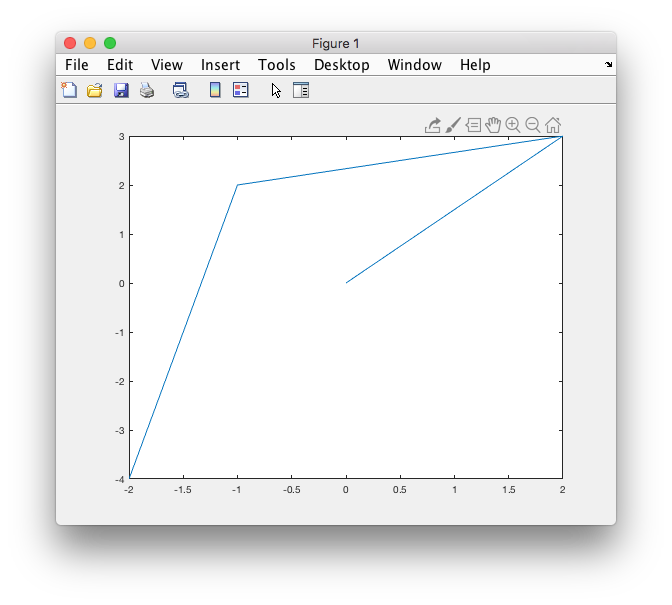
\includegraphics[width=12cm]{figura.png}
\caption{Ventana gráfica de Matlab. representación de los punto de la tabla \ref{tpuntos}}
\label{fig:ventana}
\end{figure}

La ventana gráfica de Matlab, tiene en su parte superior una barra de herramientas y un menú desplegable con funciones específicas para la manipulación de los gráficos. Se aconseja leer la ayuda de Matlab sobre el uso de dichas herramientas.

Una de las opciones del menú desplegable, permite guardar la figura generada como un archivo gráfico. Además, es posible mediante otra de las opciones del menú copiar la figura y pegarla posteriormente en un editor de texto\footnote{Al menos es posible hacerlo así si se trabaja en el sistema operativo Windows de Microsoft.}. Si copiamos la figura \ref{fig:ventana} y la pegamos directamente en el texto obtendríamos un gráfico como el de la figura, \ref{fig:plot}. A partir de ahora importaremos de esta manera todas las figuras que construyamos con Matlab.

\begin{figure}[h]
\centering
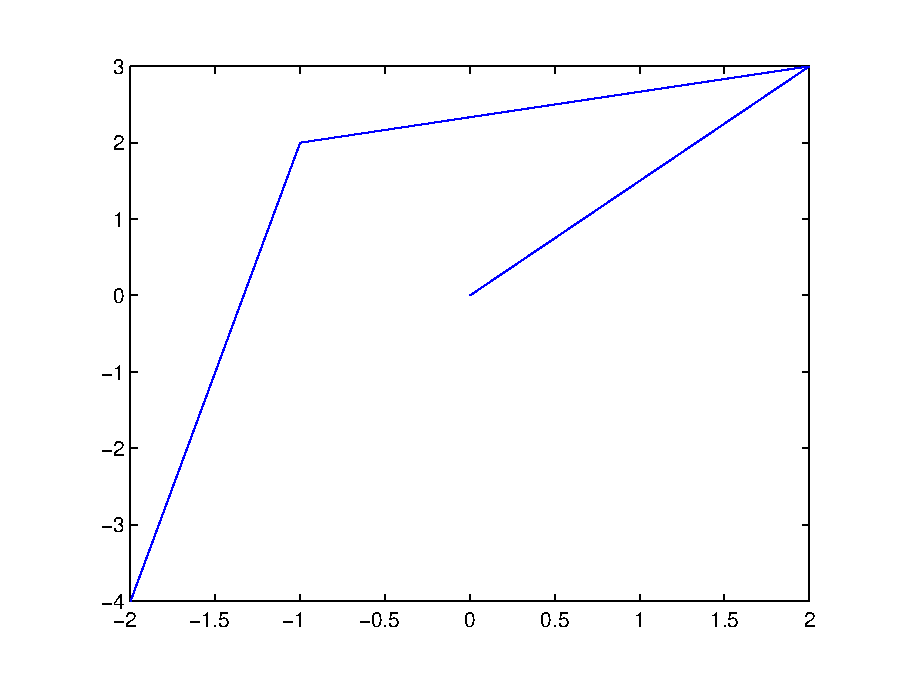
\includegraphics[width=12cm]{plot.eps}
\caption{gráfico de los puntos de la tabla \ref{tpuntos} obtenida con el comando \texttt{plot}}
\label{fig:plot}
\end{figure}
El comando plot admite un tercer parámetro de entrada. Se trata de símbolos, escritos entre comillas simples, que permiten definir: 
\begin{itemize}
\item El tipo de línea que se empleará en el gráfico. por ejemplo \texttt{plot(x,y,'-.`')} une los puntos mediante una línea de puntos y guiones.
\item El símbolo que se empleará para representar los puntos. Por ejemplo, \texttt{plot(x,y,'o')} dibuja un círculo en la posición de cada punto y no los une entre sí mediante líneas rectas.
\item El color que se empleará para dibujar. Por ejemplo, \texttt{plot(x,y,'r')}. Dibuja la gráfica en color rojo.
\end{itemize}

Si no se define este tercer parámetro, \texttt{plot} dibujará los gráficos, por defecto, en color azul, uniendo los puntos con líneas continuas y no usará ningún símbolo para dibujar los puntos individuales.
 
La tabla \ref{tcolor} muestra los símbolos disponibles para dibujar con el comando \texttt{plot}.

\begin{table}[h]
\caption{tipos de línea y color del comando \texttt{plot}}
\centering
\begin{tabular}{rc|rc|rc}
Tipo de línea&Símbolo&Tipo de punto& Símbolo &Color&Símbolo\\ 
\hline
continua&-&punto&.&azul&b\\
puntos&:&círculo&o&verde&g\\
puntos y guiones&-.&equis&x&rojo&r\\
guiones&--&más&+&cyan&c\\
&&asterisco&*&amarillo&y\\
&&diamante&d&negro&k\\
&&triangulo vértice abajo&v&blanco&w\\
&&triangulo vértice arriba&\^{}&&\\
&&triangulo vértice izquierda&\textless&&\\
&&triangulo vértice derecha&\textgreater&&\\
&&triangulo vértice arriba&\^{}&&\\
&&cuadrado&s&&\\
&&pentágono&p&&\\
&&hexágono&h&\\
\hline
\end{tabular}
\label{tcolor}
\end{table} 

Se puede combinar un símbolo de cada tipo en un mismo \texttt{plot}. Así por ejemplo si queremos representar los datos de la tabla \ref{tpuntos} unidos mediante una línea de puntos,
\begin{verbatim}
plot(x,y,':')
\end{verbatim} 

Si queremos que pinte solo los puntos sin unirlos con líneas y en color rojo,
\begin{verbatim}
plot(x,y,'.r')
\end{verbatim}

Si queremos que pinte los puntos representados por triángulos con el vértice hacia arriba, unidos mediante una línea continua y en color negro,

\begin{verbatim}
plot(x,y,'-^k')
\end{verbatim}

La figura \ref{fig:tplot} muestra los resultados de las combinaciones de símbolos que acabamos de describir.

\begin{figure}[h]
\centering
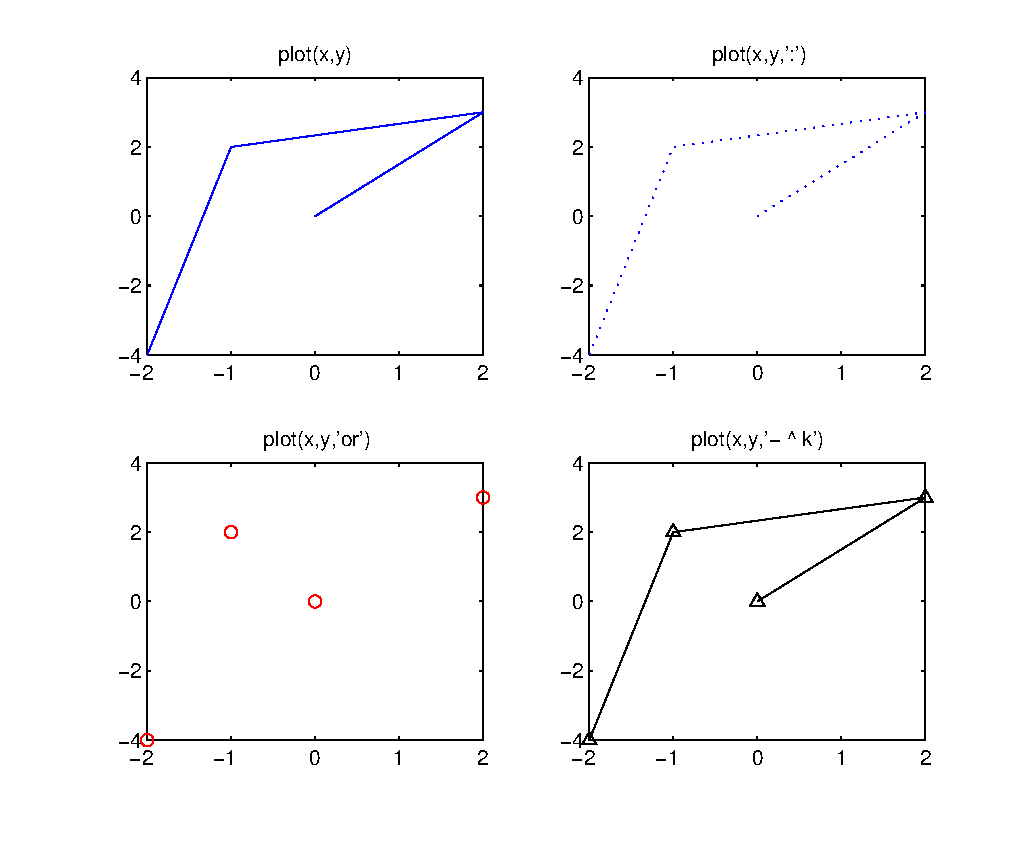
\includegraphics[width=12cm]{tiposplot.eps}
\caption{Datos de la tabla \ref{tpuntos} representados mediante distintos tipos de líneas y colores}
\label{fig:tplot}
\end{figure}

\paragraph{Figuras.} Cada vez que escribimos en la ventana de comandos de Matlab, un comando gráfico como por ejemplo \texttt{plot} Matlab comprueba si existe alguna figura (ventana de gráficos) abierta. Pueden darse entonces tres situaciones distintas. 

\begin{enumerate}
\item No hay ninguna figura abierta. Matlab crea entonces una figura nueva y representa en ella el gráfico pedido.
\item Hay una figura abierta. Matlab empleará dicha figura para representa el gráfico pedido. Por defecto, Matlab borrará cualquier gráfico anterior que contuviese la figura.
\item Existe más de una figura abierta. Matlab empleará para dibujar la llamada figura activa, que corresponde con la figura que se haya utilizado o que se haya seleccionado por última vez con el ratón.
\end{enumerate}

Es posible crear varias figuras distintas empleando directamente el comando \texttt{figure}. Cada vez que lo introduzcamos en la ventana de comandos, Matlab creará una figura nueva asignándole un número (figura 1, 2 ,3 etc.). Si empleamos el comando \texttt{figure}, seguido de un número entre paréntesis, \texttt{figure(25)}, Matlab creará una nueva figura asignándole dicho número y si ya existe la figura la convertirá en la figura activa.
El siguiente script muestra un ejemplo del uso de \texttt{figure} y \texttt{plot} combinados.

% \begin{lstlisting}
% % este script  (figuras.m)muestra el uso de los comandos figure y plot 
% % para pintar varias funciones se aconseja copiarlo y probarlo en 
% % Matlab para entender mejor cómo funciona.

% % vamos a pintar un trozo de la función e^x, en concreto para el 
% % intervalo x=[0,1]

% % Construimos un vector de 100 puntos equiespaciados en el intervalo [0,1]

% x=linspace(0,1,100);

% % calculamos el valor de la funcion e^x para los puntos construidos,

% y1=exp(x);

% % pintamos los puntos y frente a x,

% plot(x,y1) % plot ha construido una figura en Matlab, la figura 1.

% % Construimos una segunda figura en Matlab
% figure % se ha construido la figura 2

% % construimos una tercera figura 
% figure % se ha construido la figura 3


% % calculamos los valores que tomará la función sin(2*pi*x) para los 
% % puntos x del intervalo [0,1] que ya tenemos
% y2=sin(2*pi*x);

% % hacemos activa la figura 2
% figure(2)
% % pintamos en esta figura los puntos de la función sin...

% plot(x,y2)

% % volvemos a hacer activa la figura 1
% figure(1)
% % pintamos ahora los puntos de la de la función y=e^x, pero invertidos 
% % x frente a y, La grafica anterior se borra y es sustituida por la nueva,
% plot(y1,x)

% % creamos una nueva figura asignándole un numero al crearla,
% figure(13)

% % volvemos activar la figura 3
% figure(3)

% % volvemos a pintar, ahora en la figura 3, la función y=e^x,
% plot(x,y1)

% % volvemos a activar la figura 13 y pintamos en ella de nuevo la 
% % funcion sin..

% figure(13)
% plot(x,y2)
% \end{lstlisting}

Como se ha señalado antes, cualquier comando gráfico que se ejecute borra por defecto el contenido anterior de la figura activa. Es posible cambiar este comportamiento, empleando para ello el comando \texttt{hold}. Si en la ventana de comandos escribimos \texttt{hold on}, a partir de ese momento la ventana activa mantendrá cualquier gráfico que contenga y añadirá a este los nuevos gráficos que se creen. Este comportamiento se mantiene hasta que vuelva a escribirse en la ventana de comandos la sentencia \texttt{hold off}. El siguiente script muestra un ejemplo del uso de este comando y La figura \ref{fig:sico} el gráfico resultante.

% \begin{lstlisting}
% % ejemplo de uso de hold on para representar dos funciones en el mismo
% % gráfico

% % vamos a representar las funciones seno y coseno en el intervalo [-pi, pi]

% % creamos un vector de 100 puntos en el intervalo,
% x=[-pi:2*pi/99:pi];

% % calculamos el valor de la función seno sobre los puntos x
% seno=sin(x);

% % calculamos el valor de la función coseno sobre los puntos x
% coseno=cos(x);

% % pintamos la funcion seno, con linea continua azul
% plot(x,seno)

% % le pedimos que mantenga el gráfico creado
% hold on

% % pintamos encima la función coseno en linea continua roja

% plot(x,coseno,'r')

% \end{lstlisting}


\begin{figure}[h]
\centering
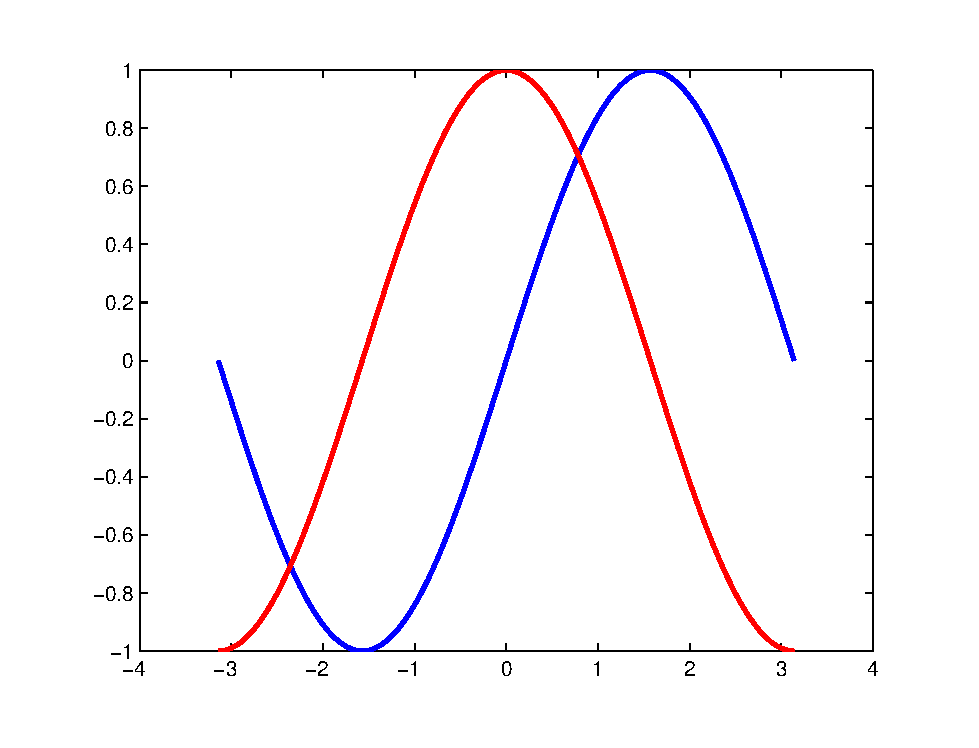
\includegraphics[width=12cm]{sico.eps}
\caption{gráficas de las funciones seno y coseno en el intervalo $(-\pi, \pi)$. Representadas en la misma figura, usando el comando \texttt{hold on}.}
\label{fig:sico}
\end{figure}

Es posible también incluir varios gráficos separados en la misma figura. 
Para ello se emplea el comando \texttt{subplot(i,j,k)}. Este comando divide la figura en un total de $i\times j$ gráficos y activa el situado en la posición $k$, las posiciones se cuentan fila a fila de arriba a abajo. El siguiente script muestra el uso del comando \texttt{subplot} La figura \ref{fig:subplot} muestra el resultado obtenido.
\begin{figure}[h]
\centering
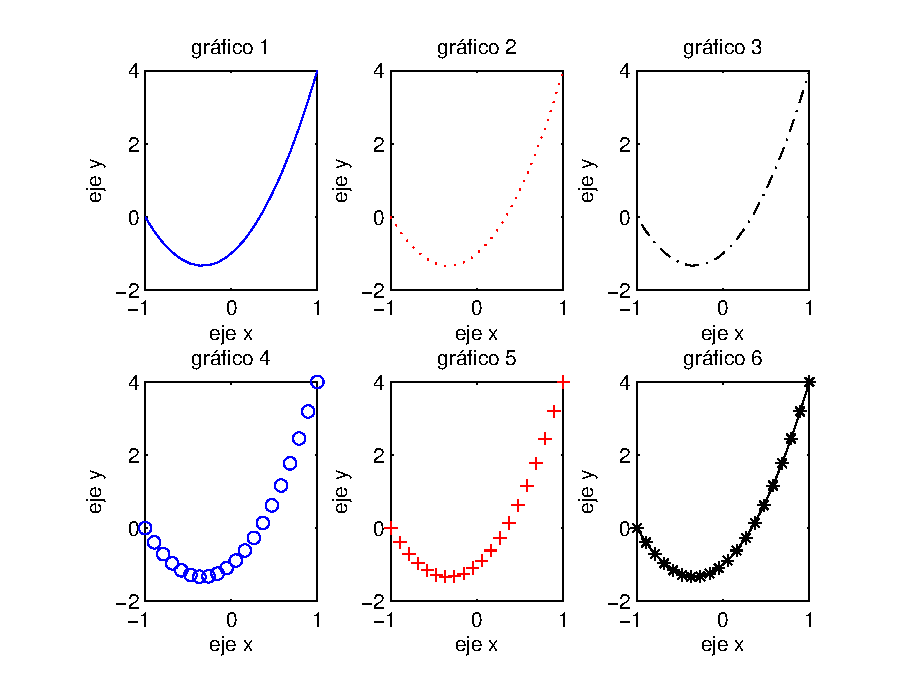
\includegraphics[width=12cm]{subplot.eps}
\caption{Ejemplo de empleo del comando subplot}
\label{fig:subplot}
\end{figure}


% \begin{lstlisting}
% % Este script muestra el uso del comando subplot

% % vamos a crear una figura con 2X3=6 gráficas, se disponen en la figura 
% % como si fueran los elementos de una matriz...
% % usamos el comando subplot de modo que cree el primer eje de los 6
% subplot(2,3,1)

% % definimos un vector x de puntos equiespacios en el intervalo (-1,1)
% x=linspace(-1,1,20);

% % calculamos los valores de polinomio 3x^2+2^x-1
% y=3*x.^2+2*x-1;

% % dibujamos la función en los ejes
% plot(x,y)

% % Añadimos rótulos a los ejes
% xlabel('eje x')
% ylabel('eje y')
% % Añadimos un titulo al grafico
% title('gráfico 1')

% % Generamos los siguientes ejes (a la derecha del anterior)
% subplot(2,3,2)
% % dibujamos la misma función pero ahora en linea discontinua roja
% plot(x,y,':r')

% % Añadimos rótulos a los ejes
% xlabel('eje x')
% ylabel('eje y')
% % Añadimos un titulo al grafico
% title('gráfico 2')

% % Generamos los siguientes ejes (a la derecha del anterior)
% subplot(2,3,3)
% % dibujamos la misma función pero ahora en linea de punto y raya negra
% plot(x,y,'-.k')

% % Añadimos rótulos a los ejes
% xlabel('eje x')
% ylabel('eje y')
% % Añadimos un titulo al grafico
% title('gráfico 3')

% % Generamos los siguientes ejes (debajo de los primeros)
% subplot(2,3,4)
% % dibujamos la misma función pero ahora solo con circulos azules
% plot(x,y,'o')

% % Añadimos rótulos a los ejes
% xlabel('eje x')
% ylabel('eje y')
% % Añadimos un titulo al grafico
% title('gráfico 4')

% % Generamos los siguientes ejes (a la derecha del anterior)
% subplot(2,3,5)
% % dibujamos la misma función pero ahora solo con cruce rojas
% plot(x,y,'+r')

% % Añadimos rótulos a los ejes
% xlabel('eje x')
% ylabel('eje y')
% % Añadimos un titulo al grafico
% title('gráfico 5')

% % Generamos los últimos ejes (a la derecha del anterior)
% subplot(2,3,6)
% % dibujamos la misma función pero ahora en linea continua y asteriscos
% % negros
% plot(x,y,'-*k')

% % Añadimos rótulos a los ejes
% xlabel('eje x')
% ylabel('eje y')
% % Añadimos un titulo al grafico
% title('gráfico 6')
% \end{lstlisting}


En el ejemplo, se ha hecho usos de algunos comandos para gráficos que permiten introducir títulos. Estos son: 

\texttt{title}, introduce un titulo a un gráfico, por ejemplo,
\begin{verbatim}
title('gráfico de temperaturas')
\end{verbatim}

\texttt{xlabel}, añade un rótulo al eje x, por ejemplo,

\begin{verbatim}
xlabel('tiempo en segundos')
\end{verbatim}

\texttt{ylabel} añade un rótulo al eje y , por ejemplo,
\begin{verbatim}
ylabel('distancia en metros')
\end{verbatim}

\subsection{Gráficos en 2D} \index{Gráficos! Comandos gráficos en 2D}
Hasta ahora, hemos visto tan solo el comando \texttt{plot}, que nos ha servido para introducir las capacidades gráficas en Matlab. Como hemos visto, plot permite representar gráficamente colecciones de datos en dos dimensiones. Hay otros muchos comandos que permiten obtener representaciones \emph{especializadas} de datos en dos dimensiones. A continuación veremos algunos de los más destacables.
\begin{figure}[h]
\centering
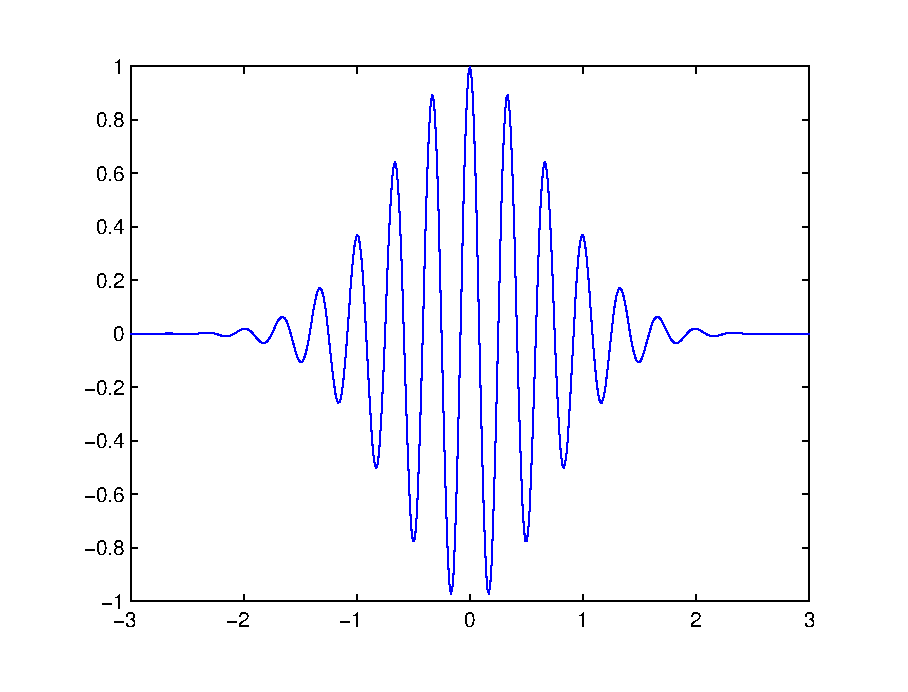
\includegraphics[width=12cm]{wave.eps}
\caption{Ejemplo de empleo del comando \texttt{fplot}}
\label{fig:wave}
\end{figure} 

\paragraph{fplot.} Permite dibujar directamente una función en un intervalo de valores. El nombre de la función hay que introducirlo entre comillas simples y el intervalo como un vector de dos componentes. Por ejemplo,

\begin{verbatim}
>> fplot('exp(-x.^2).*cos(6*pi*x)',[-3 3])
\end{verbatim}

dibuja la función,
\begin{equation*}
f(x)=e^{-x^2}\cos(6\pi x)
\end{equation*}

en el intervalo $[-3,3]$ (figura \ref{fig:wave}).

 
\paragraph{semilogx.} El comando \texttt{semilog} representa el eje de las x en escala logarítmica, Es decir, en lugar de representar frente a la variable $x$, se representa frente a $\log_{10}(x)$. Si dibujamos empleando este tipo de gráfico la función $y=\log_{10}(x)$ deberíamos obtener una línear recta de pendiente unidad. La figura \ref{fig:slx} muestra el resultado, empleando para las \emph{equis} el intervalo $(0,1)$.
\begin{verbatim}
>> x=linspace(0,1,100);
>> y=log10(x);
>> semilogx(x,y)
>> grid on
\end{verbatim}

\begin{figure}[h]
\centering
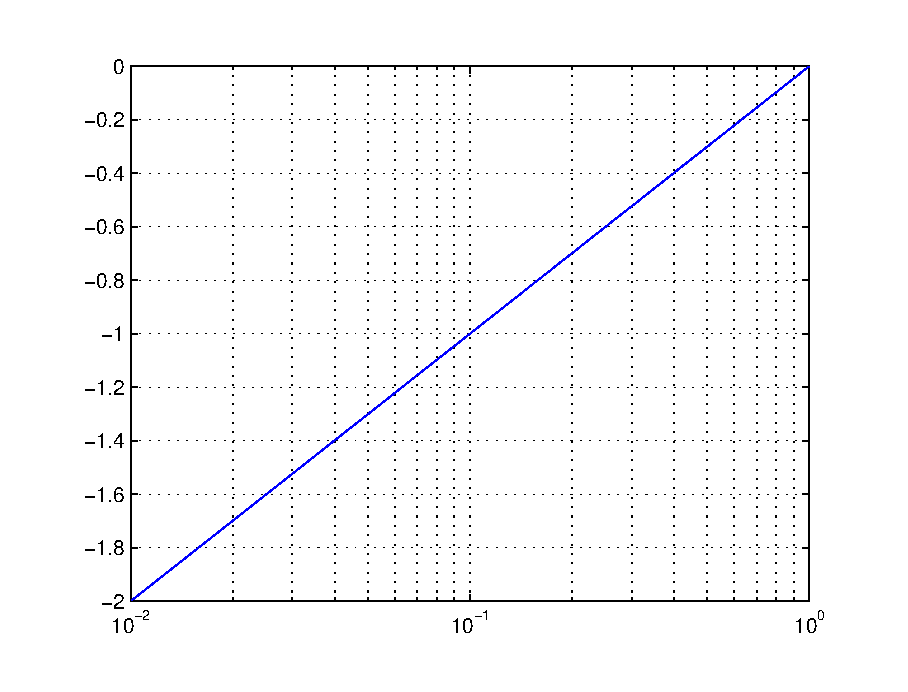
\includegraphics[width=10cm]{slx.eps}
\caption{Representación de la función $y=\log_{10}(x)$ empleando el comando \texttt{semilogx}}
\label{fig:slx}
\end{figure} 

Un par de observaciones sobre este ejemplo: En primer lugar las divisiones del eje x aparecen marcadas como potencias de 10. Como estamos representando empleando el logaritmo decimal de la variable x, las divisiones se corresponden con el exponente de la potencia de 10 de cada división, $\log_{10}(10^n)=n$.

En segundo lugar hemos empleado un nuevo comando gráfico; se trata del comando \texttt{grid}. Este comando añade una retícula al gráfico de modo que sea más fácil ver los valores que toman las variables en cada punto de la gráfica. \texttt{grid on},añade la retícula y \texttt{grid off} la retira.

\paragraph{semilogy.} Análoga al anterior, simplemente que ahora es el eje y el que se representa en escala logarítmica. En este caso será si representamos la función $y=10^x$ cuando obtengamos una línea recta,

\begin{verbatim}
>> x=linspace(0,1,100);
>> y=10.^x;
>> semilogy(x,y)
>> grid on
\end{verbatim}

\begin{figure}[h]
\centering
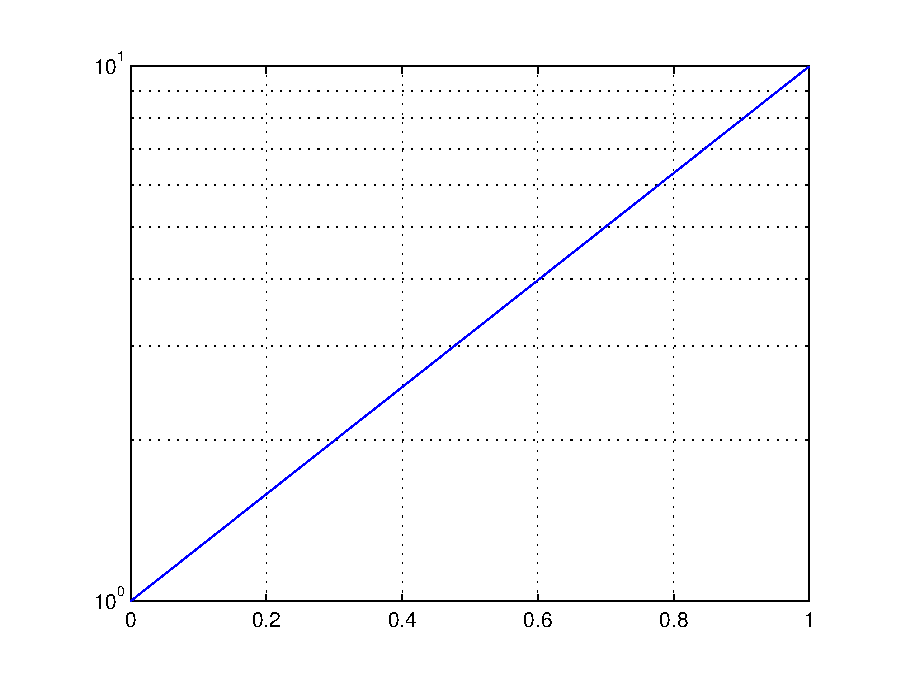
\includegraphics[width=10cm]{sly.eps}
\caption{Representación de la función $y=10^x$ empleando el comando \texttt{semilogy}}
\label{fig:sly}
\end{figure}

\paragraph{loglog.} Análoga a las anteriores, \texttt{loglog(x,y)} representa \texttt{y} frente a \texttt{x} empleando en ambos ejes una escala logarítmica.


\paragraph{polar.} Representa funciones en coordenadas polares \texttt{polar(theta,r}. La primera variable es un ángulo en radianes y la segunda el correspondiente radio. La figura \ref{fig:esp} muestra la espiral,
\begin{equation*}
r=2\cdot\sqrt{\theta}
\end{equation*}

Para el intervalo angular $[0,8\pi]$.
 
\begin{verbatim}
>> theta=linspace(0,8*pi,100);
>> r=2*theta;
>> polar(theta,r)
>> r=sqrt(theta);
>> polar(theta,r)
\end{verbatim}

\begin{figure}[h]
\centering
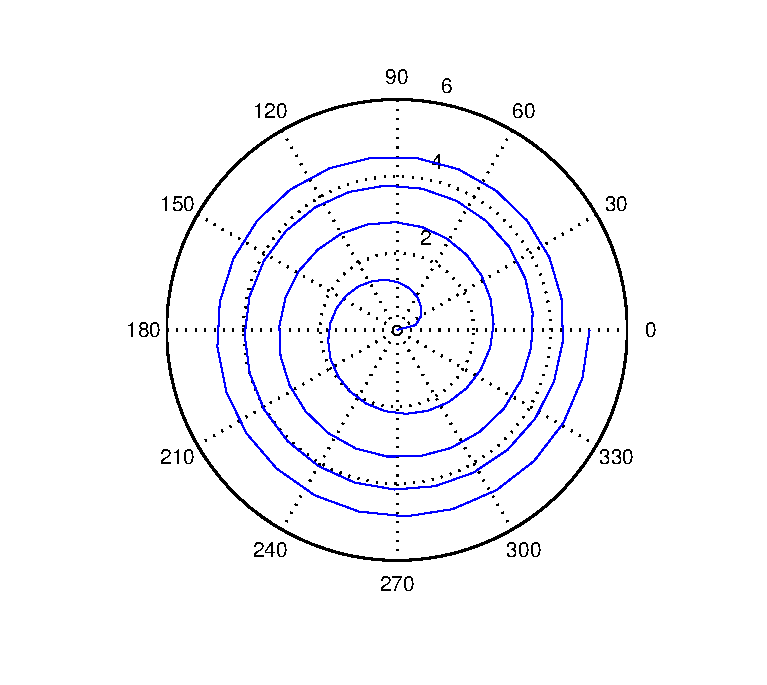
\includegraphics[width=10cm]{esp.eps}
\caption{Representación de la función $r=\sqrt{\theta}$ empleando el comando \texttt{polar}}
\label{fig:esp}
\end{figure}

\paragraph{stem, bar, stairs.} En los tres casos, se obtienen representaciones \emph{discretas} de un conjunto de datos. \texttt{stem} representa los datos mediante líneas verticales que parten del eje  x y llegan hasta el valor correspondiente de y. Las líneas van rematadas por un círculo. \texttt{bar} Emplea barras solidas verticales  y \texttt{stairs} realiza una representación en escalera. La figura \ref{fig:sbs} muestra el resultado de dibujar, empleando estos tres tipos de gráficos, los datos correspondientes al número de coches por cada 1000 habitantes en 2007 para cincuenta países distintos (los datos se guardaban en una matriz llamada auto\_50\_2007),

\begin{verbatim}
>> subplot(1,3,1)
>> stem(auto_50_2007)
>> subplot(1,3,2)
>> bar(auto_50_2007)
>> subplot(1,3,3)
>> stairs(auto_50_2007)
\end{verbatim}

\begin{figure}[h]
\centering
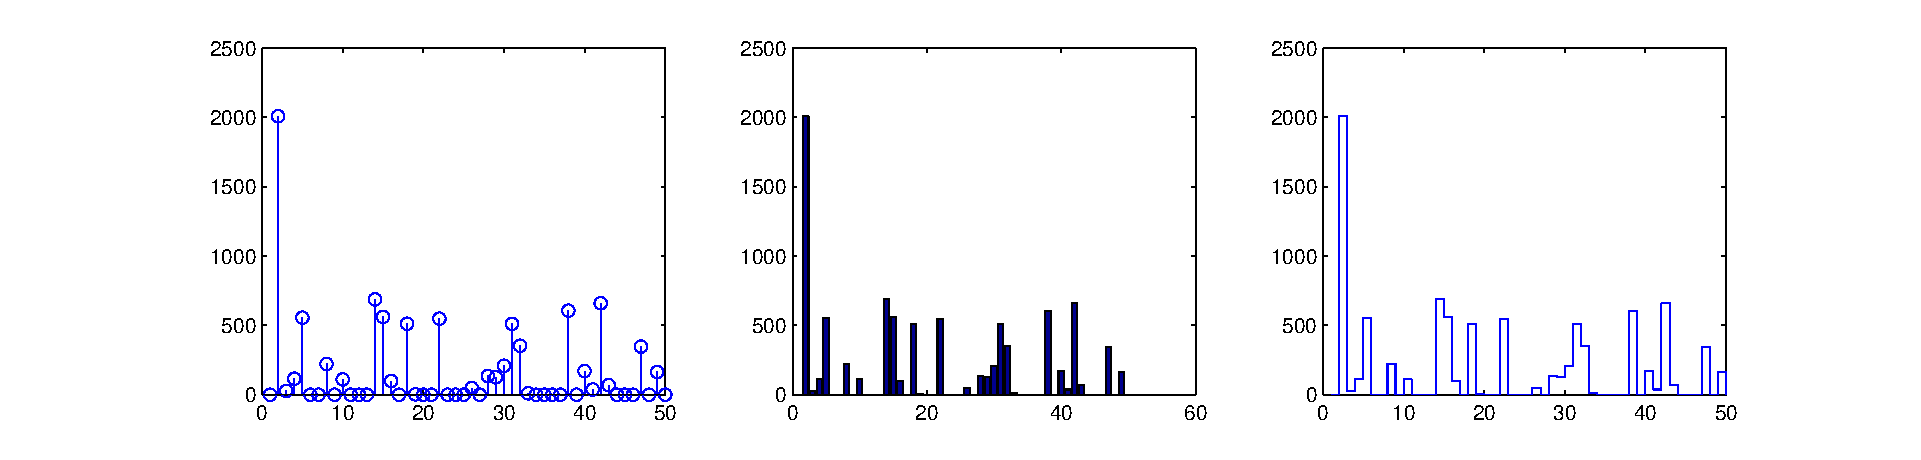
\includegraphics[width=15cm]{sbs.eps}
\caption{Comparción entre los comandos \texttt{stem}, \texttt{bar} y \texttt{stairs} representando la misma colección de datos.}
\label{fig:sbs}
\end{figure}

\paragraph{hist.} Este comando permite dibujar el histograma de una colección de datos. El histograma es una forma de representar cuantas veces se repite un datos, o más exactamente cuantos datos de la colección caen dentro de un intervalo dado. La función \texttt{hist(x,n)} admite dos parámetros de entrada, un vector de datos \texttt{x} y un valor entero \texttt{n} que representa el número de intervalos en que se dividirá el rango de valores de \texttt{x}, para obtener el histograma. Si no se introduce esta segunda variable, Matlab por defecto divide el rango de los datos en 10 intervalos. Veamos un ejemplo de uso de hist, empleando los datos del ejemplo anterior relativos a número de coches por cada mil habitantes. Representaremos el histograma para un total de 213 países. Para tener una idea, del rango de los dato, calculamos el valor mínimo y máximo de los datos disponibles,
\begin{verbatim}
>> minimo=min(auto2007)
minimo =

     0

>> maximo=max(auto2007)

maximo =

   874
\end{verbatim}

El rango va de $0$ a $879$ automóviles por cada mil habitantes. La figura \ref{fig:hist} muestra los histogramas obtenidos sin indicar el número de intervalos, ---por lo que se tomarán 10---, tomando 5 intervalos y tomando 20.

\begin{verbatim}
>> subplot(1,3,1)
>> hist(auto2007)
>> subplot(1,3,2)
>> hist(auto2007,5)
>> subplot(1,3,3)
>> hist(auto2007,20)
>> subplot(1,3,1)
>> title('10 intervalos')
>> subplot(1,3,2)
>> title('5 intervalos')
>> subplot(1,3,3)
>> title('20 intervalos')
\end{verbatim}

\begin{figure}[h]
\centering
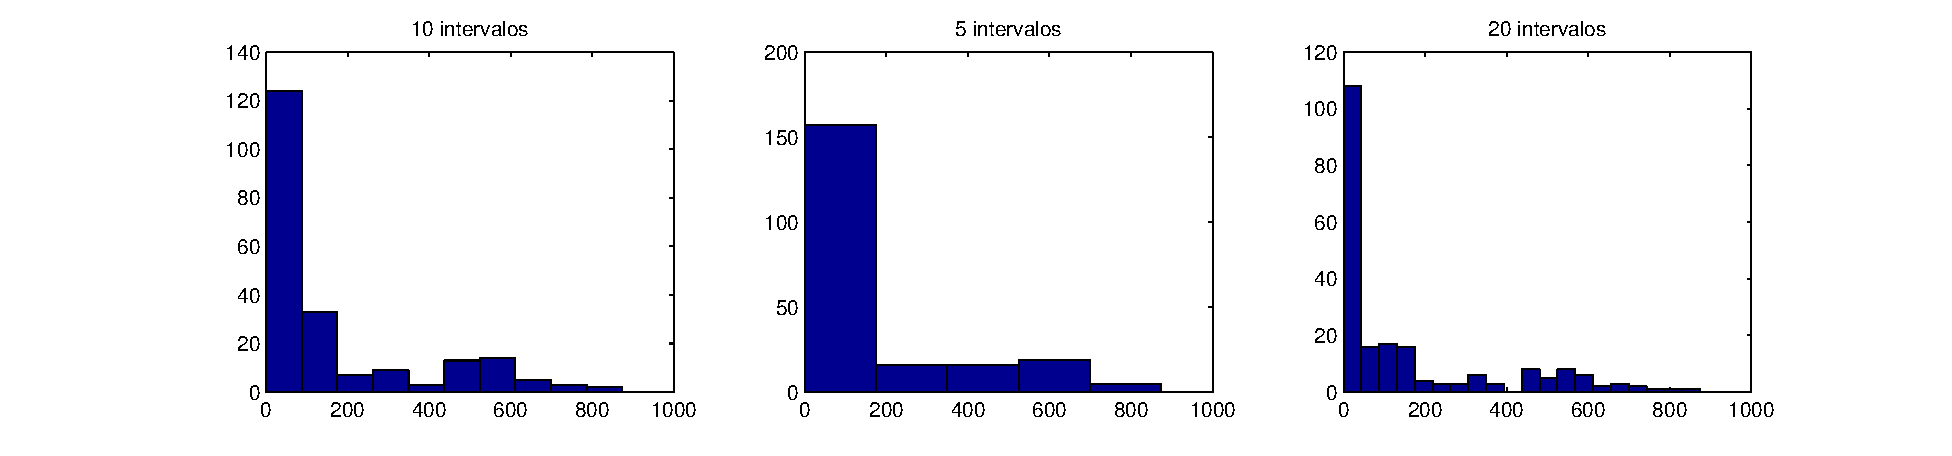
\includegraphics[width=15cm]{hist.eps}
\caption{histogramas del número de automóviles por cada 1000 habitantes para 213 países}
\label{fig:hist}
\end{figure}

La interpretación del los histogramas depende lógicamente del número de intervalos. En el caso de 10 intervalos, estos dividen los datos en grupos de aproximadamente 100 coches. Si observamos el histograma resultante, podemos concluir que hay unos 120 países en los que hay entre 0 y 100 automóviles por cada 1000 habitante, unos 30 países en los que hay entre 100 y 200 automóviles por cada 1000 habitante, etc. Si miramos el siguiente histograma, en el que se han empleado tan solo 5 intervalos, los grupos son ahora de aproximadamente 200 coches. La primera barra de este segundo histograma establece que hay unos 150 países en los que hay entre 0 y 200 coches por cada 1000 habitantes. Resultado que corresponde a la suma de los de dos primeros intervalos del histograma anterior. Para el tercer histograma los intervalos son ahora de 50 automóviles, lo que permite observar más en detalle que en los histogramas anteriores la distribución de vehículos: 110 países tienen menos de 50 automóviles por cada 1000 habitantes.

\paragraph{plotyy.} Este comando permite representar dos gráficas en la misma figura de modo que comparten el mismo eje x y cada una tiene su propio eje y. La figura \ref{fig:plotyy} muestra el resultado del siguiente ejemplo,

\begin{verbatim}
>> x1=linspace(0,10,100);
>> x2=linspace(0,12,50);
>> y1=x1.^2;
>> y2=x2.^(2/3);
>> plotyy(x1,y1,x2,y2)
>> grid on
\end{verbatim}

\begin{figure}[h]
\centering
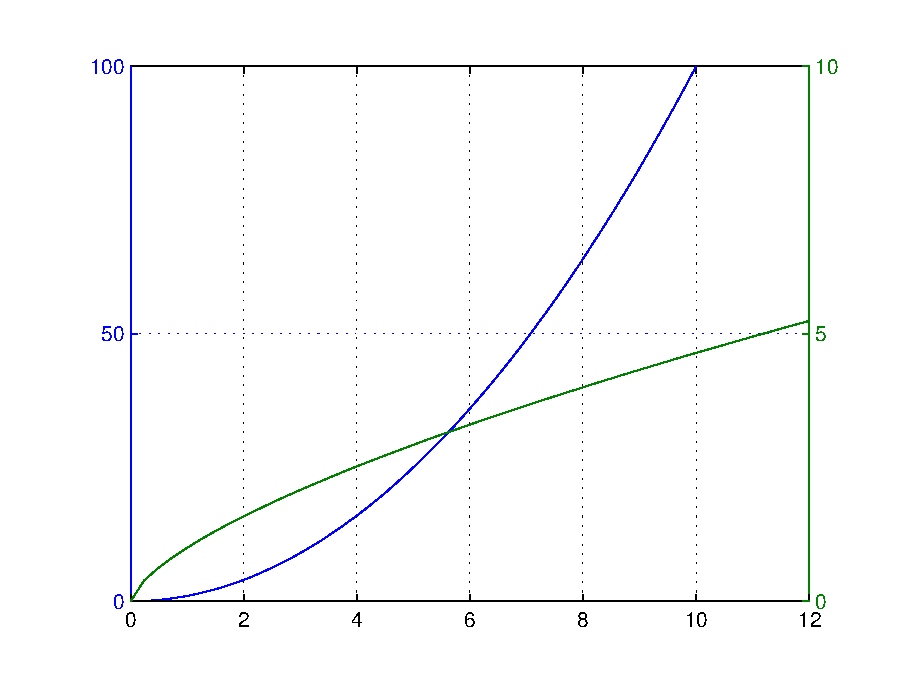
\includegraphics[width=10cm]{plotyy.eps}
\caption{Ejemplo de uso de la función \texttt{plotyy}}
\label{fig:plotyy}
\end{figure}

\paragraph{quiver.} Esta función de Matlab permite dibujar vectores en el plano. En realidad está pensada para dibujar campos vectoriales, con lo que hay que manejarla con cierto cuidado. En primera aproximación diremos que \texttt{quiver} necesita 5 variables de entrada: la coordenada $x$ del origen del vector, la coordenada $y$ del origen del vector, la componente $x$ del vector y la componente $y$ del vector, por último, un factor de escala al que daremos el valor $0$ para que dibuje los vectores a su tamaño real, sin modificar su escala. Por ejemplo si queremos dibujar el vector $\vec{v}=(1,2)$ situado en el origen de coordenadas,
\begin{verbatim}
quiver(0,0,1,2,0)
\end{verbatim}

Si queremos representar el mismo vector pero situado en el punto $(3,-1)$,
\begin{verbatim}
>>quiver(3,-1,1,2,0)
\end{verbatim}

Podemos dibujar un conjunto de vectores con quiver, para ello empleamos como variables de entradas vectores, en lugar de escalares; un vector que contenga las posiciones $x$ del los orígenes, un segundo vector que contenga la posiciones $y$ de los orígenes, un tercer vector que contenga las componentes $x$ de los vectores y un cuarto que contenga las componentes $y$, por último añadiríamos el parámetro de escala $0$, que sigue siendo un escalar.

Por tanto, si queremos dibujar a la vez los dos vectores de los ejemplos anteriores,

\begin{verbatim}
>>quiver([0 3],[0 -1],[1 1],[2 2],0)
\end{verbatim}

La figura \ref{fig:quiver} muestra los resultados del ejemplo que acabamos de ver,

\begin{figure}[h]
\centering
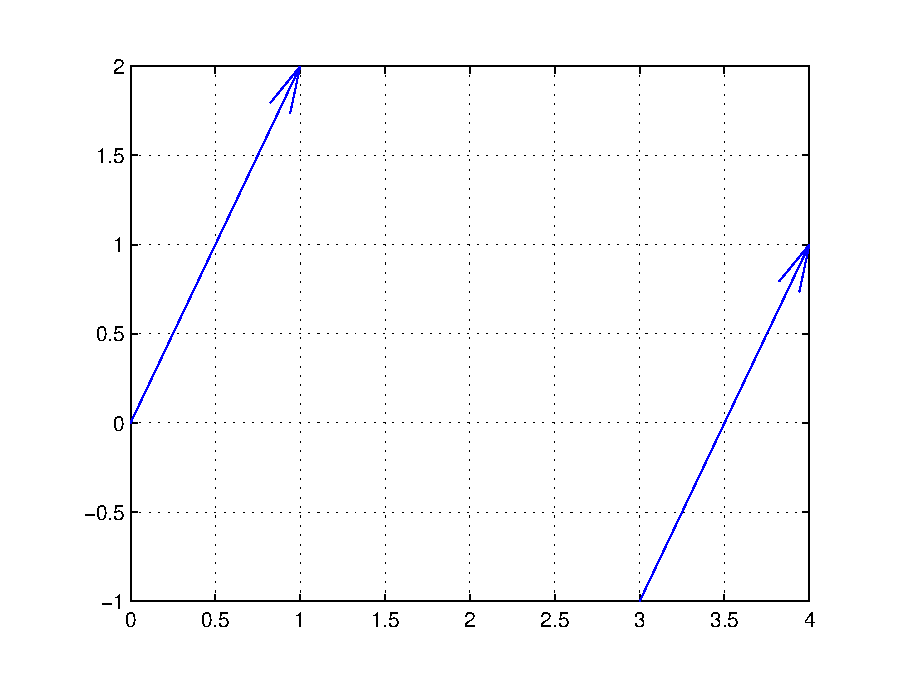
\includegraphics[width=10cm]{quiver.eps}
\caption{Ejemplo de uso de la función \texttt{quiver}}
\label{fig:quiver}
\end{figure}

\paragraph{errorbar.} Permite añadir barras de  error a un gráfico de puntos experimentales. Supongamos que tenemos la siguiente tabla (\ref{vel}) de resultados de la medida de la velocidad de un móvil frente al tiempo,


\begin{table}[h]
\caption{Resultados experimentales de la medida de la velocidad de un móvil}
\centering
\begin{tabular}{ccc}
\hline
\hline
tiempo &velocidad& incertidumbre\\ 
$t$ (s)&$v$ (m/s)& $\pm \Delta v$ (m/s)\\
\hline
0&0&0\\
1&2.8&0.8\\
2&4.0&0.8\\
3&4.3&0.9\\
4&4.2&0.9\\
5&4.8&1.0\\
6&6.3&1.0\\
7&7.9&1.0\\
8&8.9&1.1\\
9&9.0&1.1\\
10&8.7&1.1\\
\hline
\hline
\end{tabular}
\label{vel}
\end{table} 

La primera columna representa el instante de tiempo en que se tomó la medida, la segunda columna representa el valor medido de la velocidad y la tercera columna la incertidumbre de cada medida de velocidad.

podemos emplear el comando \texttt(errorbar) para representar la velocidad frente al tiempo, añadiendo una barra de error en cada medida que represente la incertidumbre,

\begin{verbatim}
>> vel=[0 2.8 4.0 4.3 4.2 4.8 6.3 7.9 8.9 9.0 8.7]
vel =

  Columns 1 through 7

         0    2.8000    4.0000    4.3000    4.2000    4.8000    6.3000

  Columns 8 through 11

    7.9000    8.9000    9.0000    8.7000

>> inc=[0 0.8 0.8 0.9 0.9 1.0 1.0 1.0 1.1 1.1 1.1]
inc =

  Columns 1 through 7

         0    0.8000    0.8000    0.9000    0.9000    1.0000    1.0000

  Columns 8 through 11

    1.0000    1.1000    1.1000    1.1000

>> t=0:10
t =

     0     1     2     3     4     5     6     7     8     9    10

>> errorbar(t,vel,inc)
>> xlabel('tiempo s')
>> ylabel('velocidad m/s')
\end{verbatim}

EL resultado se muestra en la figura \ref{fig:error}. Es interesante hacer notar que la longitud total de cada barra de error es el doble del valor de la incertidumbre correspondiente al punto. Por ejemplo para $t=1s, v+\Delta v=2.8\pm 0.8 m/s$ la longitud de la barra de error es $2\cdot \Delta v=1.6 m/s$). El comando \texttt{errobar}, puede también emplearse para representar incertidumbres asimétricas. Para ello  es preciso suministrar dos vectores uno \texttt{U} para dibujar la parte superior de la barra de error y otro \texttt{L} para dibujar la parte inferior; \texttt{errorbar(x,y,L,U)}. 

\begin{figure}[h]
\centering
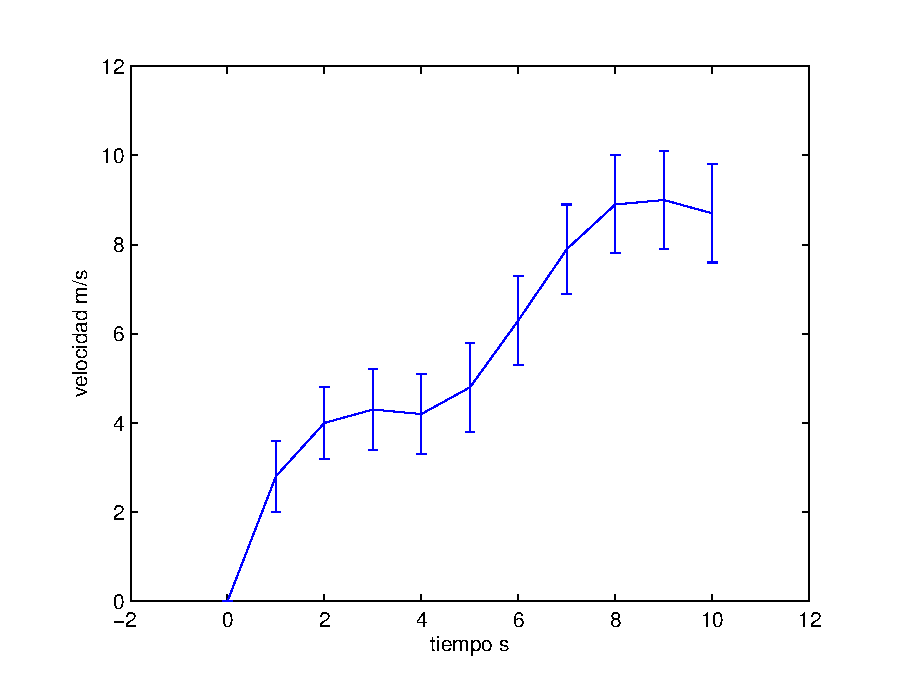
\includegraphics[width=11cm]{error.eps}
\caption{Datos de la tabla \ref{vel} representados empleando el comando \texttt{errorbar}}
\label{fig:error}
\end{figure}

\subsection{Gráficos en 3D.} \index{Gráficos! Comandos gráficos en 3D}En tres dimensiones es posible representar dos tipos de gráficos: puntos y curvas, análogos a los representados en dos dimensiones y además superficies en el espacio.

\paragraph{plot3.} Para dibujar líneas y puntos Matlab emplea los mismos comandos que hemos descrito para dos dimensiones, añadiendo al nombre de comando la terminación \texttt{3} para indicar que se trata de un gráfico en tres dimensiones. Así por ejemplo el comando \texttt{plot3} nos permite dibujar puntos y curvas en el espacio. El manejo es idéntico al de \texttt{plot}, simplemente que ahora es preciso añadir un vector que contenga los datos de la tercera coordenada, z. 

Por ejemplo, podemos representar la curva,
\begin{align*}
y&=\sin(2\pi x)\\
z&=\cos(2\pi x)
\end{align*}

Para ello, seleccionamos un intervalo de valores para $x \in (0,2)$, y calculamos los correspondientes valores de $y$ y $z$,

\begin{verbatim}
>> x=linspace(0,2,100);
>> y=sin(2*pi*x);
>> z=cos(2*pi*x);
\end{verbatim}

Podemos ahora representar la gráfica de nuestra función empleando el comando \texttt{plot3},
\begin{verbatim}
>> plot3(x,y,z)
>> grid on
>> xlabel('x')
>> ylabel('y')
>> zlabel('z')
\end{verbatim}

Hemos añadido los comandos \texttt{grid on}  para obtener una trama en 3D que permita ver mejor el resultado. La figura \ref{fig:muelle1} muestra la figura de Matlab obtenida, donde se ha señalado además un botón que permite rotar la figura, cambiando la vista. Para ellos, una vez pulsado el botón, basta con arrastrar el ratón sobre la figura manteniedo pulsado el boton izquierdo.  La figura \ref{fig:muelle2}, muestra la misma gráfica en 3D, pero ahora vista de frente (como si nos situáramos en el eje x). La figura \ref{fig:muelle3}, nos muestra la grafica vista desde arriba (desde el eje z), por último, la figura \ref{fig:muelle4} muestra una vista lateral de la gráfica (tomada desde el eje y).

Es posible rotar la figura par a obtener una vista concreta mediante el comando \texttt{view(Az, El)}. Este comando admite dos parámetros; \texttt{Az}, representa el azimuth o ángulo de rotación horizontal, \texttt{El}, representa el ángulo de elevación. Ambos ángulos se introducen en grados. Así, por ejemplo las vistas representadas en las figuras anteriores, se pueden obtener como,
\begin{verbatim}
>> view(90,0)
>> view(0,90)
>> view(0,0)
\end{verbatim}

\begin{figure}[h]
\centering
\subfigure[ventana gráfica \label{fig:muelle1}]{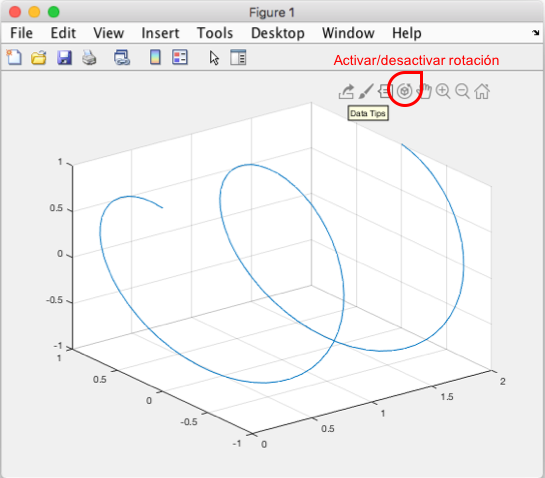
\includegraphics[width=6cm]{muelle1.png}} \qquad 
\subfigure[vista frontal (eje x) \label{fig:muelle2}]{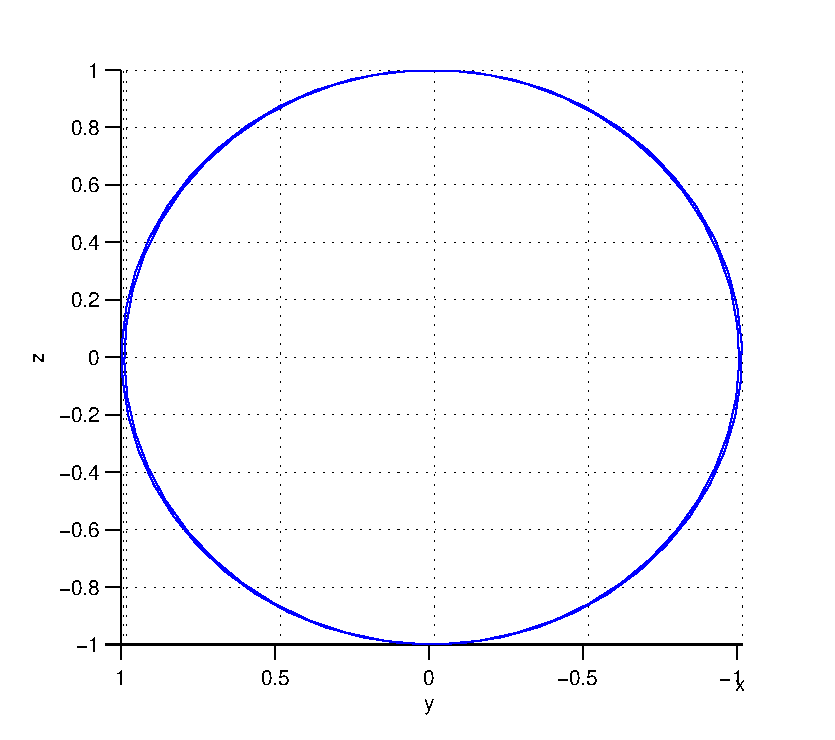
\includegraphics[width=6cm]{muelle2.eps}}\\
\subfigure[vista desde arriba (eje z) \label{fig:muelle3}]{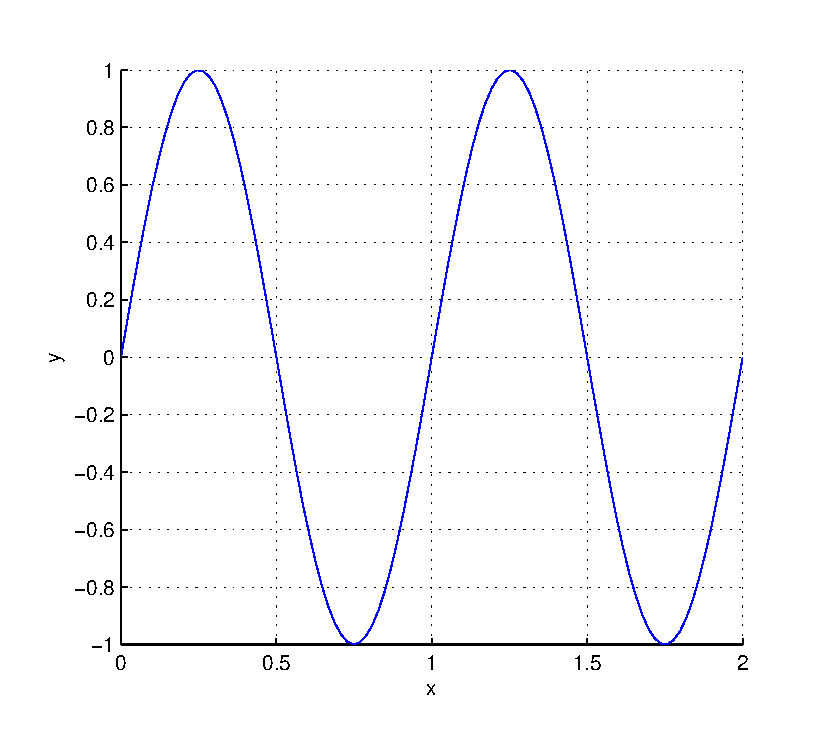
\includegraphics[width=6cm]{muelle3.eps}}\qquad
\subfigure[vista lateral (eje y)l \label{fig:muelle4}]{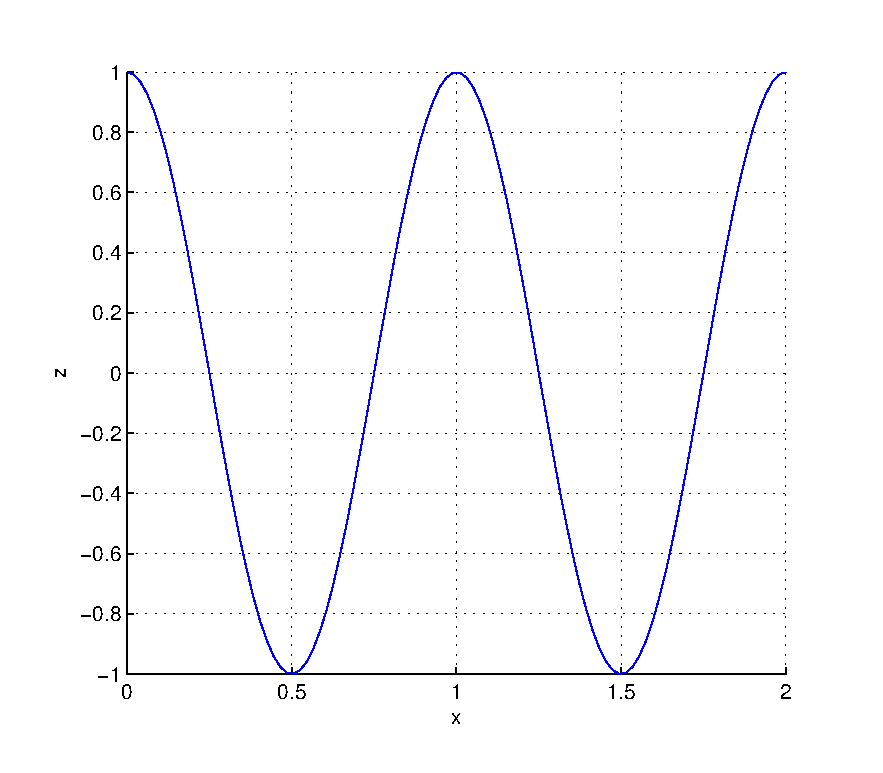
\includegraphics[width=6cm]{muelle4.eps}}\\
\caption{Gráfico en 3D y rotaciones. }
\end{figure}

\paragraph{bar3, stem3, hist3, quiver3.} Existen versiones 3D de los comandos \texttt{bar}, \texttt{stem}, \texttt{hist} y \texttt{quiver}. Su funcionamiento es similar ---aunque no siempre igual--- al de la versión 2D que vimos en la sección anterior. En algunos casos necesitan tres variables de entrada, correspondientes a las componentes (x,y,z) de los datos que se quiere representar, y en otros necesitan que los datos de entrada se le suministren en forma de matriz. Para conocer en detalle su funcinamiento, lo ideal es acudir a la ayuda de Matlab.


\paragraph{Superficies.}Para trazar superficies en el espacio, Matlab necesita en primer lugar que se defina una retícula en el plano $(x,y)$ que sirve de base sobre la que calcular los puntos z sobre los que se alzará la superficie.

Para definir dicha retícula Matlab emplea dos matrices. una de ellas $X_m$ contiene las coordenadas $x$ de los nodos de la retícula y la otra $Y_m$ las coordenadas $y$. Los elementos que ocupan la misma posición en ambas matrices, representan ---juntos--- un punto en el plano.
Matlab emplea dichas matrices como matrices de \emph{adyacencia}. Cada nodo, $(x_m(i,j),y_m(i,j)$, aparecerá en la gráfica conectado por una arista a cada uno de sus cuatros puntos vecinos, $(x_m(i-1,j),y_m(i-1,j)$, $(x_m(i,j-1),y_m(i,j-1)$, $(x_m(i+1,j),y_m(i+1,j)$, $(x_m(i,j+1),y_m(i,j+1)$.
Supongamos que empleamos las siguientes matrices, $X_m$ y $Y_m$ para definir una retícula sobre la que dibujar una superficie,

\begin{align*}
X_m=\begin{pmatrix}
0&1&2&3\\ 
0&1&2&3\\
0&1&2&3\\
0&1&2&3
\end{pmatrix},& Y_m\begin{pmatrix}
0&0&0&0\\
1&1&1&1\\
2&2&2&2\\
3&3&3&3
\end{pmatrix}\xrightarrow[nodos]{posiciones}\begin{matrix}
(0,0)&-&(1,0)&-&(2,0)&-&(3,0)\\
\vert&&\vert&&\vert&&\vert\\ 
(0,1)&-&(1,1)&-&(2,1)&-&(3,1)\\
\vert&&\vert&&\vert&&\vert\\
(0,2)&-&(1,2)&-&(2,2)&-&(3,2)\\
\vert&&\vert&&\vert&&\vert\\
(0,3)&-&(1,3)&-&(2,3)&-&(3,3)
\end{matrix}
\end{align*}

La retícula definida por Matlab, a partir de dichas matrices tendría el aspecto que se muestra en la figura \ref{fig:mesh}. 

\begin{figure}[h]
\centering
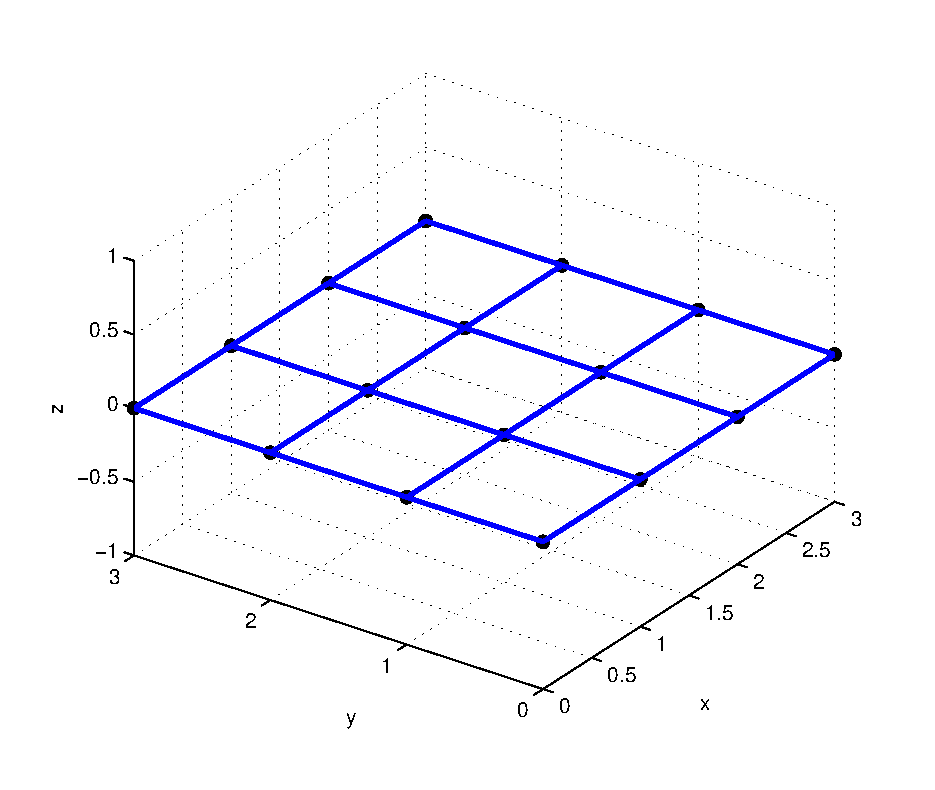
\includegraphics[width=11cm]{mesh.eps}
\caption{Retícula para representar superficies. Los puntos negros son los nodos definidos por las matrices $X_m$ e $Y_m$.}
\label{fig:mesh}
\end{figure}

Si nos fijamos en los ejes de la figura es fácil obtener las coordenadas de los nodos y comprobar como, están unidos entre sí por aristas los que ocupan posiciones adyacentes en las matrices $X_m$ e $Y_m$.

Para construir una superficie sobre la retícula, lo único que hace falta es definir una altura (z), para cada punto de la retícula. Para ello, Matlab emplea una matriz, del mismo tamaño que $X_m$ y $Y_m$. Así por ejemplo, si definimos,

\begin{equation*}
Z_m=\begin{pmatrix}
0&0&0&\\ 
0&1&2&0\\
0&3&4&0\\
0&0&0&0
\end{pmatrix}
\end{equation*}

Cada elemento de la matriz $Z_m$ representa la altura del nodo correspondiente a las posiciones marcadas por las matrices $X_m$ e $Y_m$, tal y como se muestra en la figure \ref{fig:mesh1}.

\begin{figure}[h]
\centering
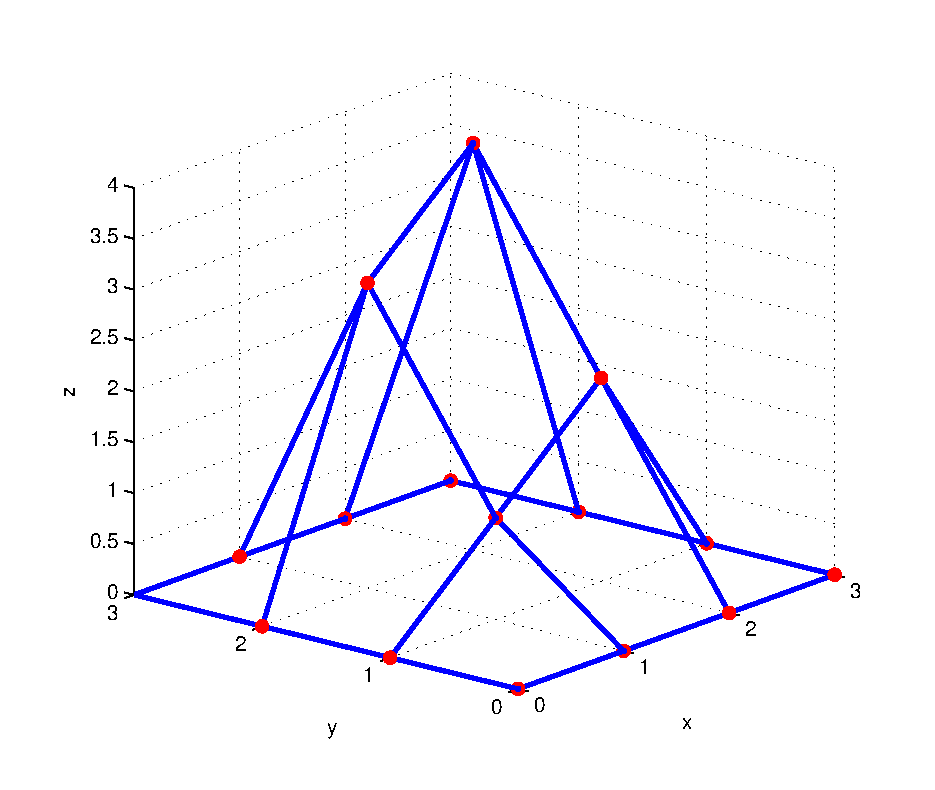
\includegraphics[width=11cm]{mesh1.eps}
\caption{Superficie elemental obtenida elevando los cuatros puntos centrales de la figura \ref{fig:mesh}.}
\label{fig:mesh1}
\end{figure}

La estructura de las matrices $X_m$ e $Y_m$ de los ejemplo anteriores, es la típica de las matrices de adyacencia de una retícula cuadrada; la matriz  $X_m$ tiene la filas repetidas y la matriz $Y_m$ tiene repetidas la columnas. En el ejemplo las matrices son cuadradas y definen una retícula de $4\times 4$ nodos. En general, podemos definir una retícula rectangular de $m\times n$ nodos. En este caso las matrices empleadas para definir la retícula tendrían dimensión $m\times n$.

Para dibujar en Matlab superficies podemos en primer lugar definir la retícula a partir de dos vectores de coordenadas empleando el comando \texttt{meshgrid}. En el ejemplo que acabamos de ver, hemos empleado una retícula que cubre el intervalo, $x\in[0,3]$ e $y\in[0,3]$. para definirlo creamos los vectores,

\begin{verbatim}
>> x=0:3
x =

     0     1     2     3

>> y=0:3
y =

     0     1     2     3
\end{verbatim}

A continuación empleamos el comando \texttt{meshgrid} para construir las dos matrices de adyacencia. Matlab se encargará de repetir las filas y columnas necesarias,

\begin{verbatim}
>> [Xm,Ym]=meshgrid(x,y)
Xm =

     0     1     2     3
     0     1     2     3
     0     1     2     3
     0     1     2     3


Ym =

     0     0     0     0
     1     1     1     1
     2     2     2     2
     3     3     3     3

\end{verbatim}

Una vez construidas las matrices de adyacencia, solo necesitamos una matriz de valores para $Z_m$. Si definimos por ejemplo,
\begin{verbatim}
>> Zm=zeros(size(Xm))

Zm =

     0     0     0     0
     0     0     0     0
     0     0     0     0
     0     0     0     0
\end{verbatim}

Podríamos representar la retícula plana de la figura \ref{fig:mesh}, empleando por ejemplo el comando \texttt{mesh(Xm, Ym, Zm)}.

\paragraph{mesh y surf.} Una vez que hemos visto como construir una retícula rectangular sobre la que construir una superficie, veamos como dibujarla con un ejemplo. Supongamos que queremos dibujar la superficie,
\begin{equation*}
z=x^3+y^2
\end{equation*}

En la región del plano, $x\in[-1.5,1.5]$, $y\in[-2,2]$. 

Igual que en el ejemplo inicial, lo primero que debemos hacer es construirnos una matrices de adyacencia que definan una retícula en la región de interés,
\begin{verbatim}
>> x=linspace(-1.5,1.5,25);
>> y=linspace(-2,2,50);
>> [Xm,Ym]=meshgrid(x,y);
\end{verbatim}

Es interesante notar que la región de interés no es cuadrada y que las matrices de adyacencia tampoco los son ($50\times 25$). Además los puntos no están espaciados igual en los dos ejes.

A continuación obtenemos la matriz de coordenadas z, aplicando la función a los puntos de la retícula,

\begin{verbatim}
>> Zm=Xm.^3+Ym.^2;
\end{verbatim}

\begin{figure}[h]
\centering
\subfigure[Función $z=x^3+y^2$ representada con \texttt{mesh}\label{fig:msh}]{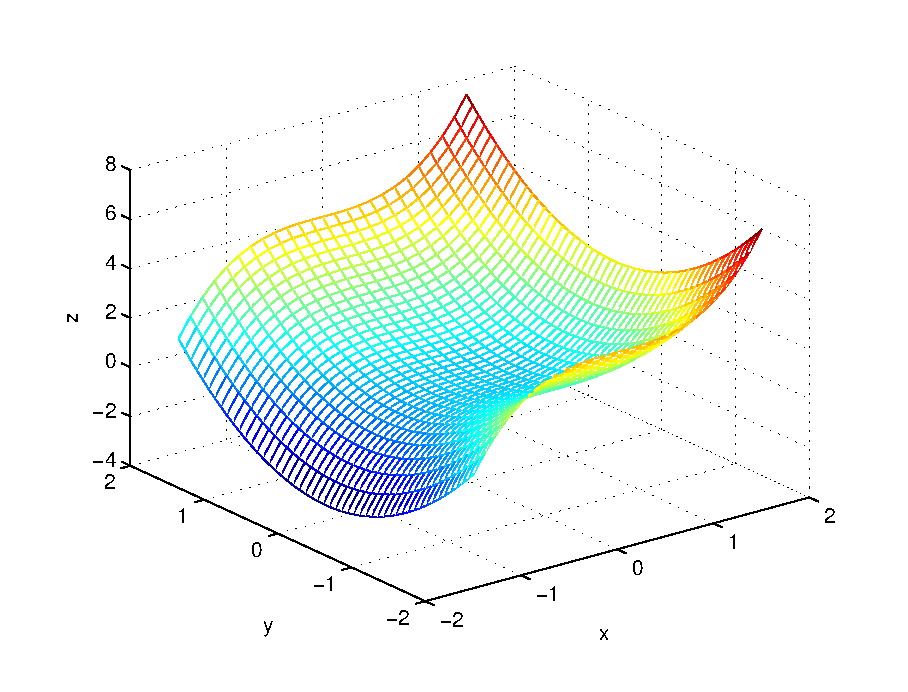
\includegraphics[width=8cm]{pa23.eps}} %\qquad 
\subfigure[Función $z=x^3+y^2$ representada con \texttt{surf} \label{fig:sur}]{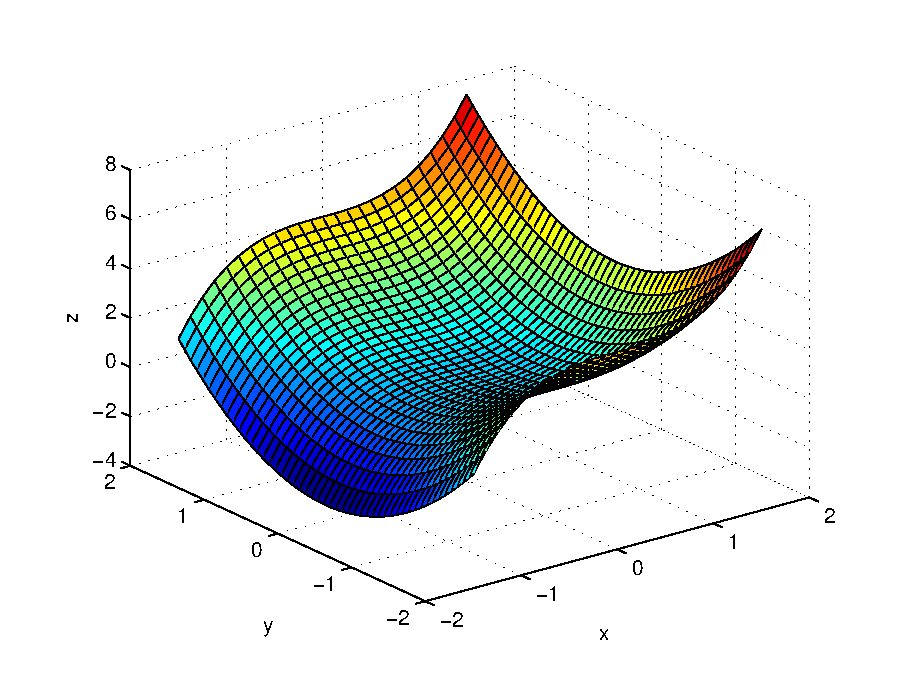
\includegraphics[width=8cm]{surf.eps}}\\
\caption{Comparación entre \texttt{mesh} y \texttt{surf}}
\end{figure}

Para representar la superficie podemos emplear el comando \texttt{mesh}. 
\begin{verbatim}
>> mesh(Xm,Ym,Zm)
\end{verbatim}

Este comando admite como variables de entrada las dos matrices de adyacencia empleadas para definir la retícula y la matriz $Z_m$ que contiene los valores calculados para la  variable z, en todos los puntos de la retícula. \texttt{mesh} traza la superficie en forma reticular, es decir, nos dibuja una malla en el espacio. El color de la malla depende del valor que toma la coordenada z. Podemos también representar la superficie haciendo uso del comando \texttt{surf}, empleando las mismas variables de entrada que en el caso de \texttt{mesh}. 
\begin{verbatim}
>> surf(Xm,Ym,Zm)
\end{verbatim}

La diferencia está en que ahora la superficie muestra las caras definidas por la malla de colores, según el valor que toma la variable $z$. la figura \ref{fig:msh} muestra el resultado de nuestro ejemplo empleando \texttt{mesh} y la figura \ref{fig:sur} muestra el resultado empleando \texttt{surf}.



Para figuras que presentan simetría radial, puede ser más conveniente, definir las retículas en coordenadas polares. así por ejemplo,

\begin{verbatim}
>> r=0:2/20:2;
>> theta=0:2*pi/36:2*pi;
>> [rm,them]=meshgrid(r,theta);
\end{verbatim}

Hemos cosntruido una retícula en las variables $r$ y $\theta$, si ahora definimos las matrices de adyacencia como las proyecciones sobre los ejes $x$ e $y$,

\begin{verbatim}
>> xm=rm.*cos(them);
>> ym=rm.*sin(them); 
\end{verbatim}

Obtenemos una retícula con simetría radial, centrada en el origen de coordenadas. Como la que se muestra en la figura, \ref{fig:retcir}.

\begin{figure}[h]
\centering
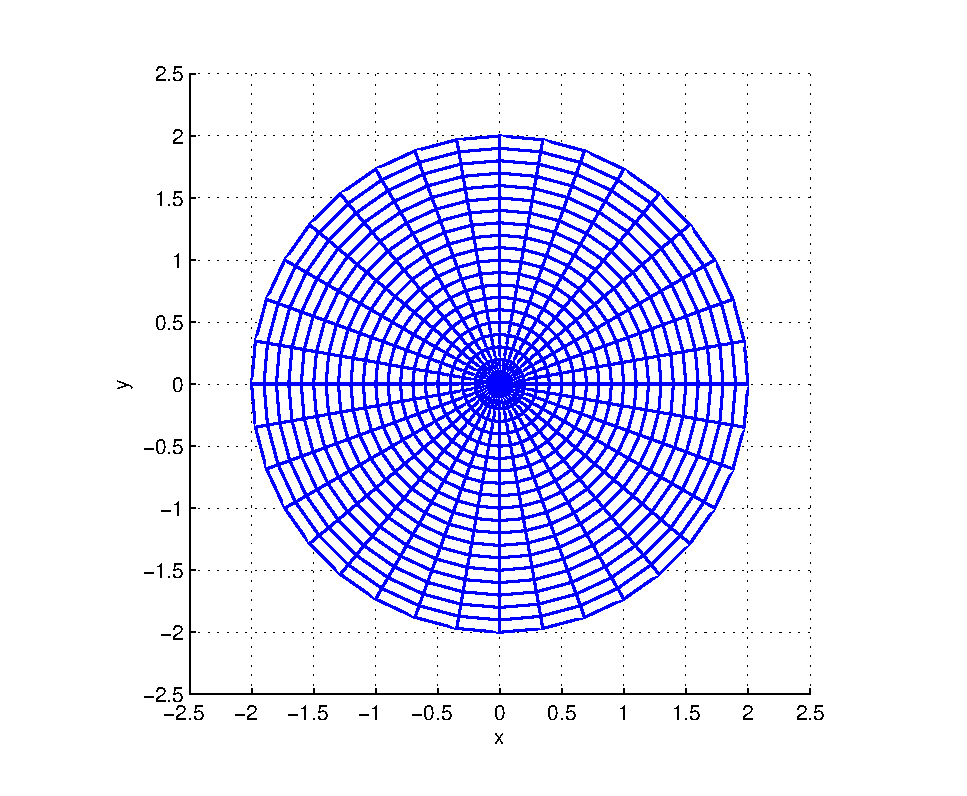
\includegraphics[width=12cm]{retcirc.eps}
\caption{retícula con simetría circular}
\label{fig:retcir}
\end{figure}

La retícula resulta muy adecuada para dibujar por ejemplo un cono (figura \ref{fig:cono}),

\begin{verbatim}
>> zm=2-sqrt(xm.^2+ym.^2);
>> mesh(xm,ym,zm)
\end{verbatim}

\begin{figure}[h]
\centering
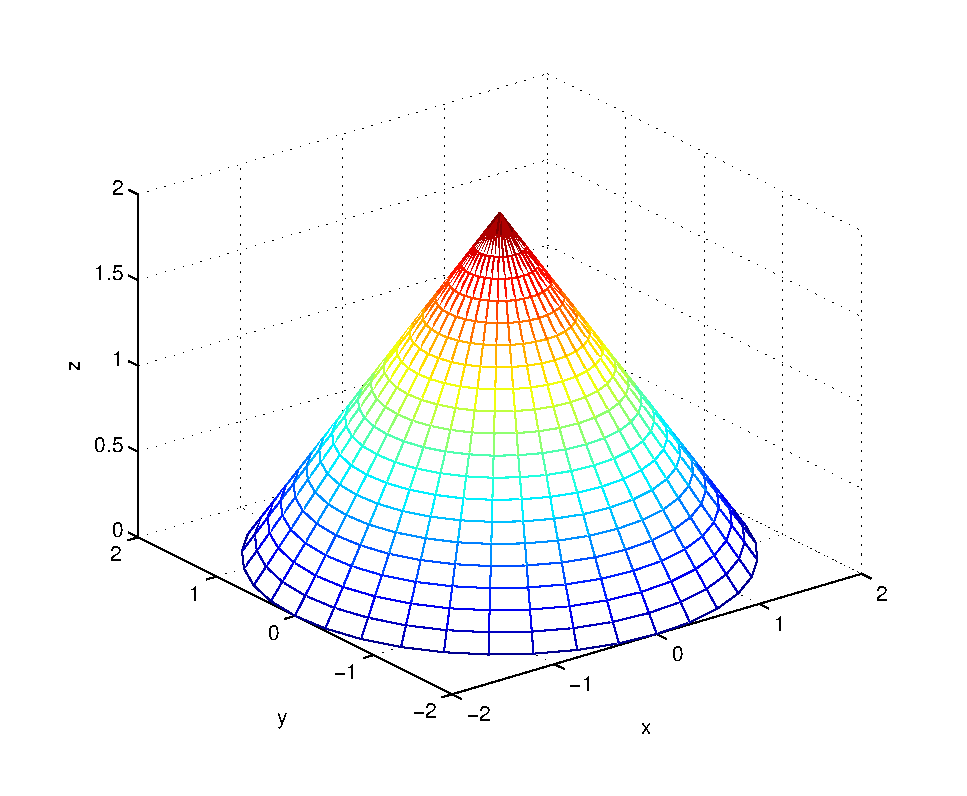
\includegraphics[width=12cm]{cono.eps}
\caption{Cono representado sobre una retícula circular}
\label{fig:cono}
\end{figure}

A continuación, se incluye el código de un script con varios ejemplos más de diseño de retículas circulares y gráficos de superficies en 3D. Los resultados se muestran en la figura \ref{fig:varios}

%\lstinputlisting{../codigo/matlab/introduccion/varios_g3d.m}

\begin{figure}[h]
\centering
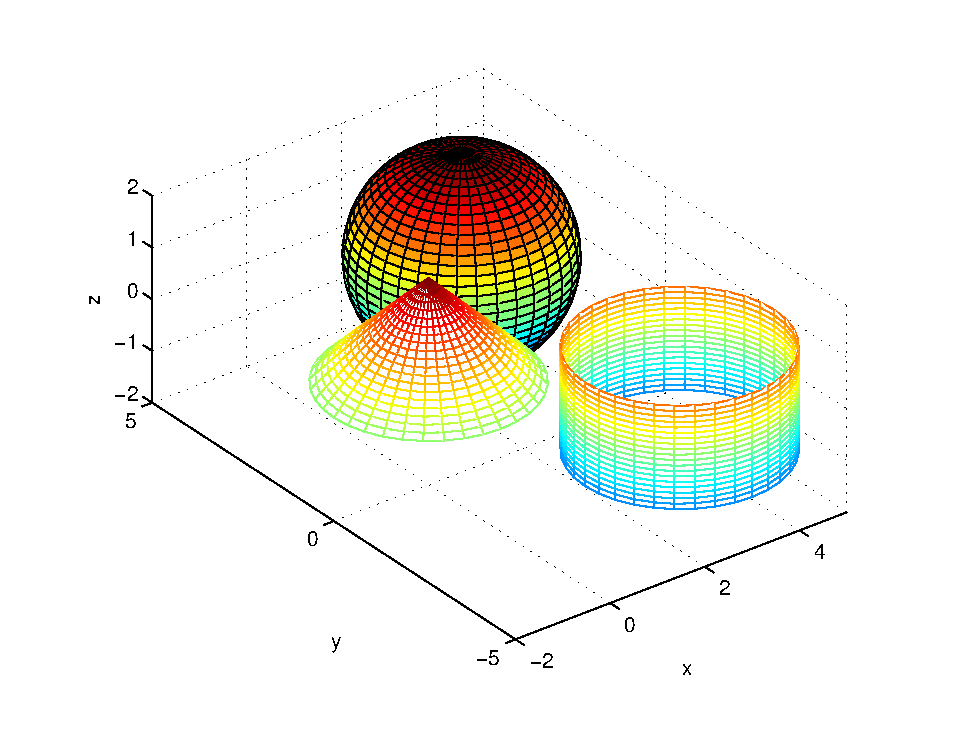
\includegraphics[width=12cm]{varios.eps}
\caption{retícula con simetría circular}
\label{fig:varios}
\end{figure}

\paragraph{contour, contour3, meshc y surfc.} Este comandos permiten obtener y dibujar las curvas de nivel de una superficie. Su uso es idéntico al de los comandos anteriores. Es decir, también necesitan que se defina una retícula en el plano $(x,y)$, y se calculen los valores que tomará  la variable z sobre los puntos de la retícula.

\begin{figure}
\centering
\subfigure[contour  \label{fig:contour}]{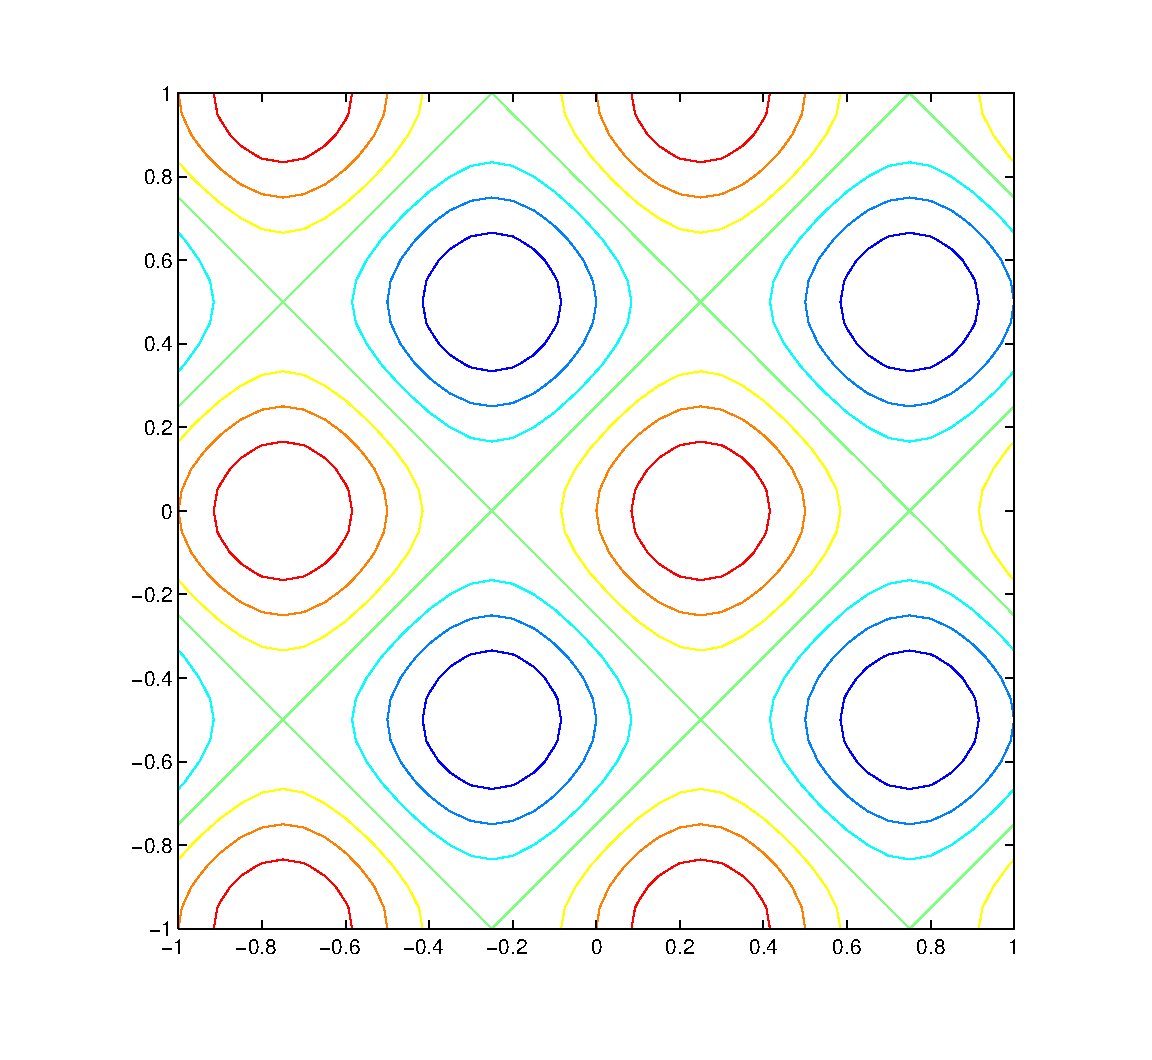
\includegraphics[width=6.5cm]{contour.eps}} \qquad 
\subfigure[contour3 \label{fig:contour3}]{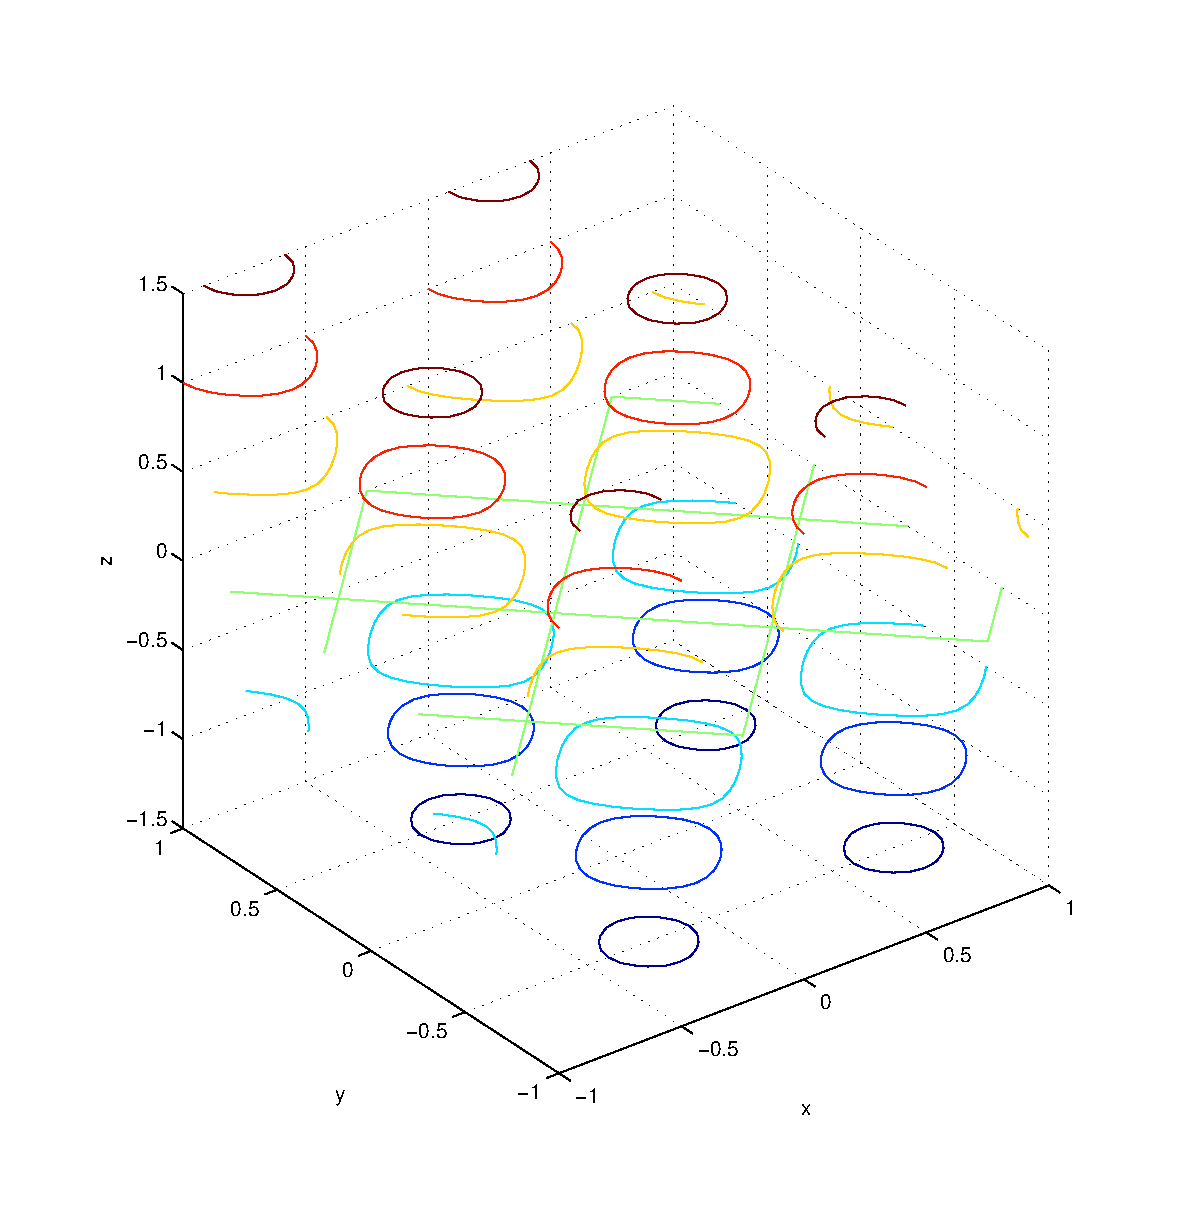
\includegraphics[width=6.5cm]{contour3.eps}}\\
\subfigure[meshc \label{fig:mesh3}]{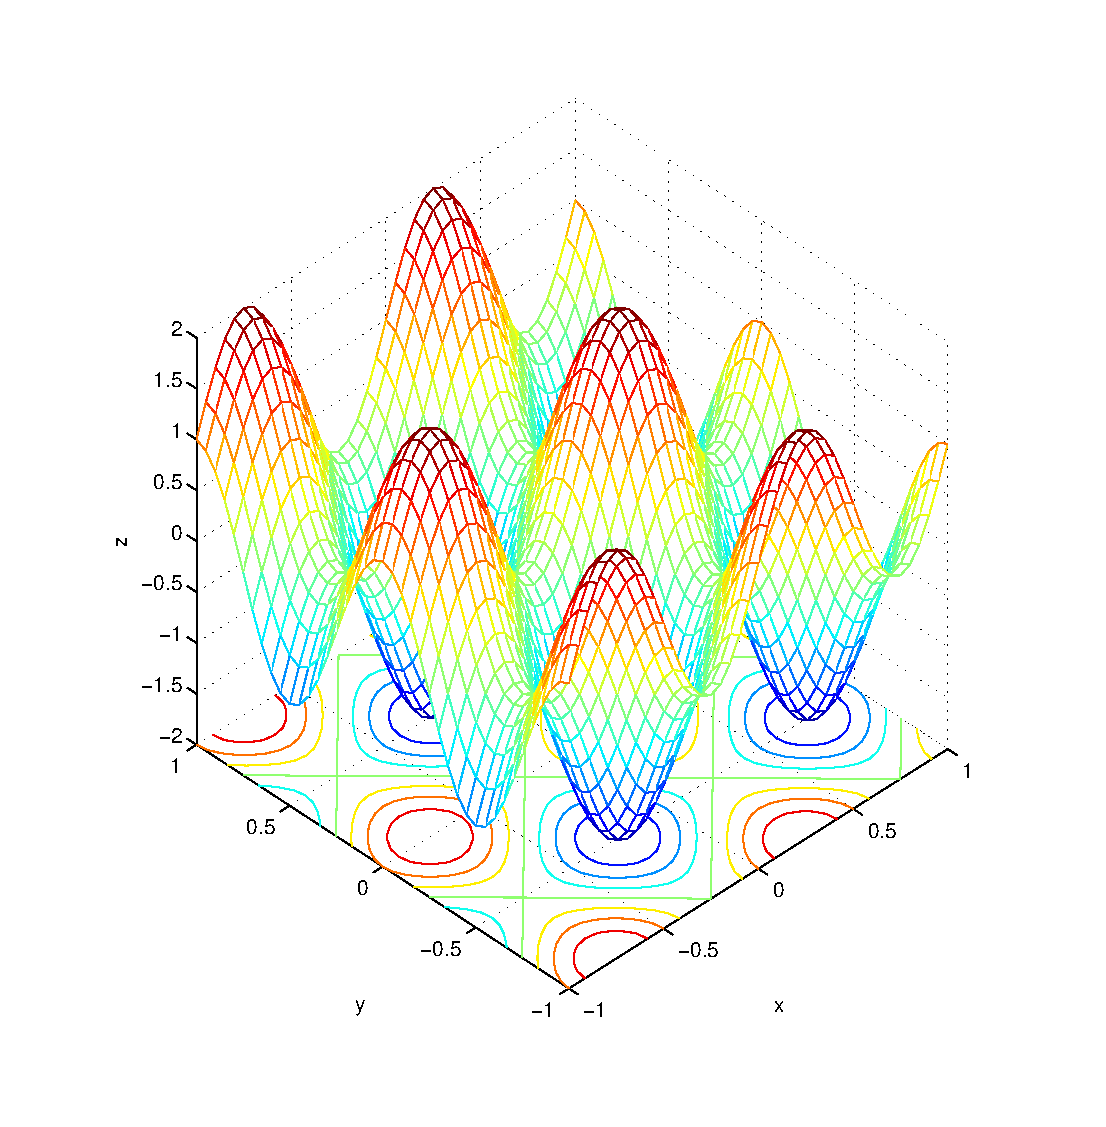
\includegraphics[width=6.5cm]{meshc.eps}}\qquad
\subfigure[surfc \label{fig:surf3}]{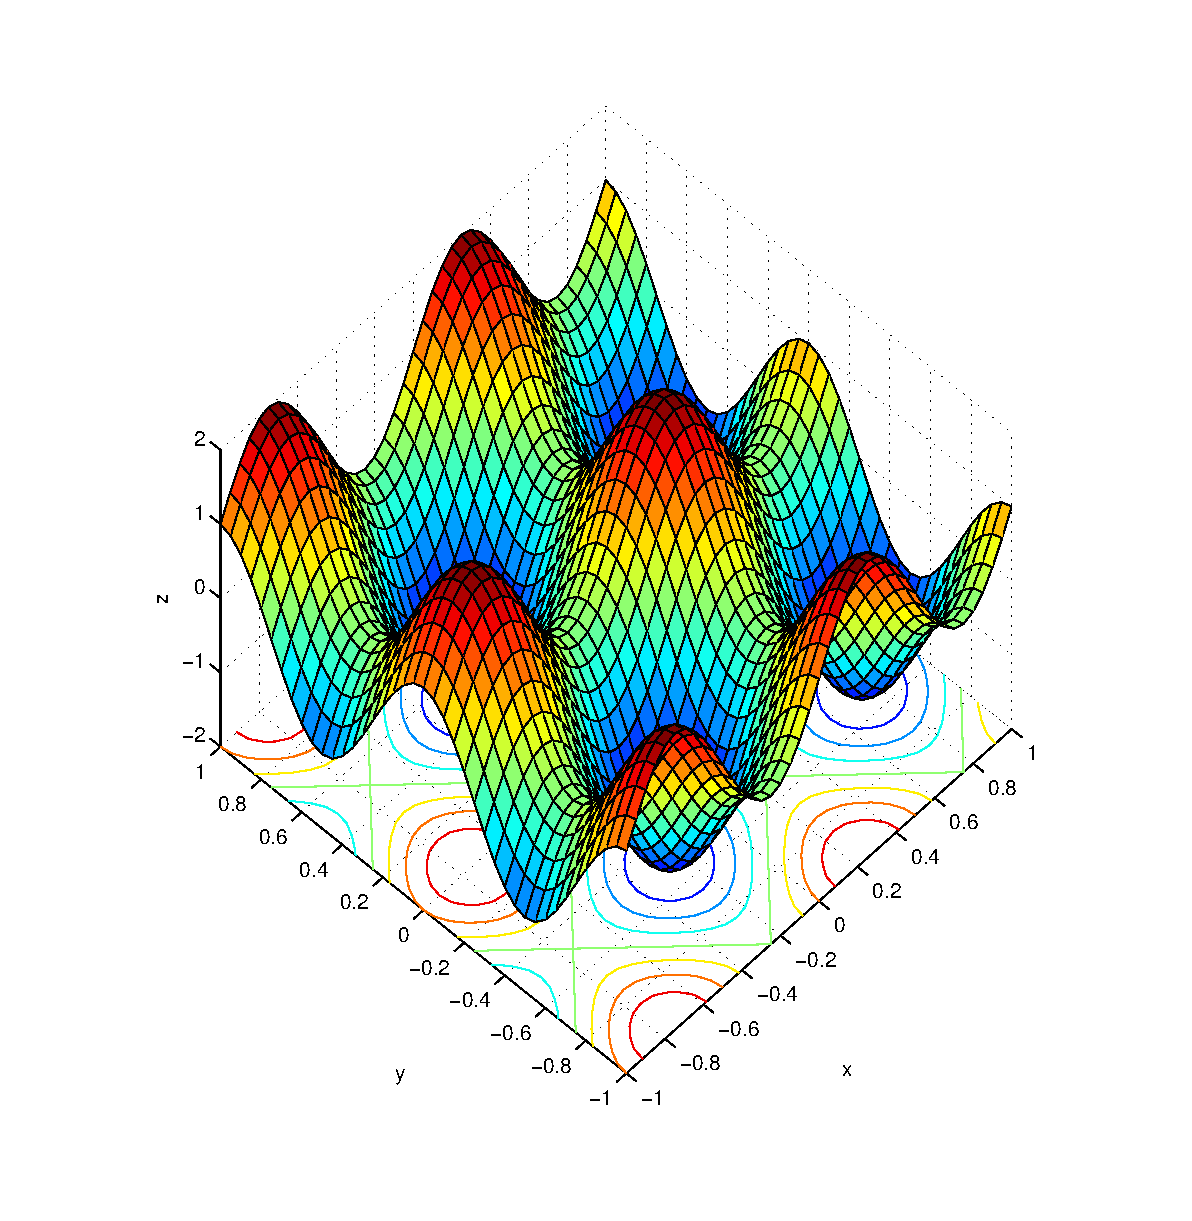
\includegraphics[width=6.5cm]{surfc.eps}}\\
\caption{Comparación entre los resultados de \texttt{contour}, \texttt{contour3}, \texttt{meshc} y \texttt{surfc}, para la obtención de las curvas de nivel de una superficie. }
\end{figure}

Veamos su funcionamiento con un último ejemplo. Obtenemos una retícula cuadrada, calculamos sobre ella los puntos de la superficie,

\begin{equation*}
z=\sin(2\pi x)+cos(2\pi y)
\end{equation*}

\begin{verbatim}
>> x=[-1:0.05:1];
>> y=x;
>> [xm,ym]=meshgrid(x,y);
>> zm=sin(2*pi*xm)+cos(2*pi*ym);
>> contour(xm,ym,zm)
>> contour3(xm,ym,zm)
>> meshc(xm,ym,zm)
>> surfc(xm,ym,zm)
\end{verbatim}



La figura \ref{fig:contour} muestra los resultados de aplicar el comando \texttt{contour}. La gráfica representa las curvas de nivel de la superficie dibujadas sobre el plano $(x,y)$. El comando \texttt{contour3} ( figura \ref{fig:contour3}) representa de nuevo las curvas de nivel, pero sitúa cada una a su correspondiente altura $z$.  Por último \texttt{meshc} y \texttt{surfc} representan la superficie y añaden en el plano $(x,y)$ la representación de las curvas de nivel correspondiente a la superficie.

Para terminar la sección dedicada a los gráficos, vamos a combinar el comando \texttt{mesh} con el comando \texttt{plot3} para dibujar una curva sobre una superficie. Tomaremos como ejemplo la superficie,
\begin{equation*}
z=\frac{sin\left((\pi x)^2+(\pi y^2)\right)}{(\pi x)^2+(\pi y^2)}
\end{equation*}

Sobre la que trazamos la curva,

\begin{equation*}
y=sin(\pi x),\\
\end{equation*}

\begin{figure}[h]
\centering
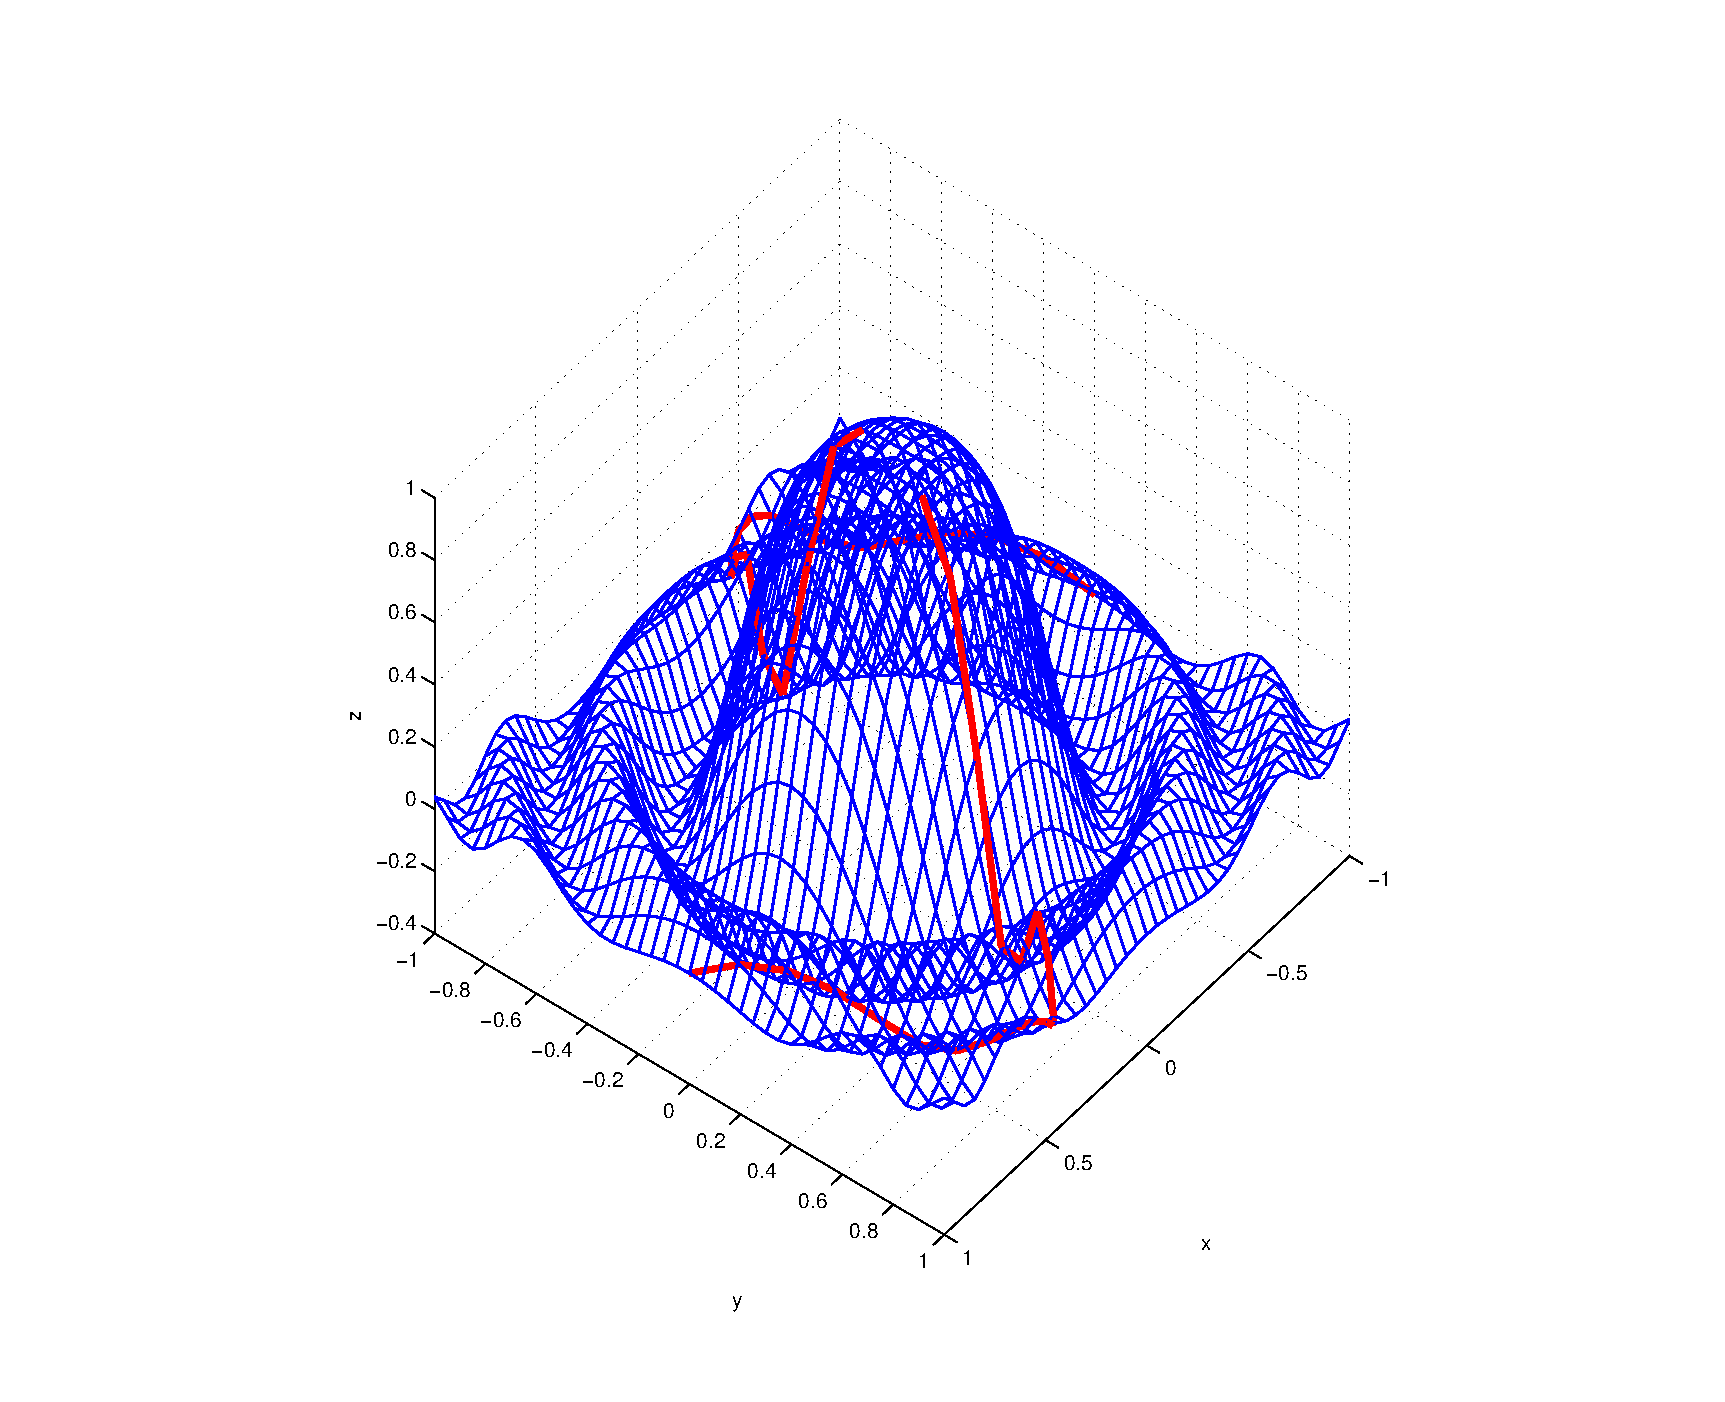
\includegraphics[width=11cm]{linsu.eps}
\caption{Curva trazada sobre una superficie}
\label{fig:cvsurf}
\end{figure}

Es decir, obtenemos el valor de los puntos $z$ de la superficie para los pares de puntos $[x, y = sin(\pi x)]$, que definen la curva trazada sobre la superficie $z$,

\begin{verbatim}
>> x=[-1:0.05:1];
>> y=x;
>> [xm,ym]=meshgrid(x,y);
>> zm=sin((pi*xm).^2+(pi*ym).^2)./((pi*xm).^2+(pi*ym).^2);
>> mesh(xm,ym,zm)
>> y=sin(pi*x);
>> z=sin((pi*x).^2+(pi*y).^2)./((pi*x).^2+(pi*y).^2);
>> hold on
>> plot3(x,y,z)
\end{verbatim}

Es importante insistir en que a lo largo de esta sección nos hemos limitado a introducir algunas de las posibilidades gráficas de Matlab. Para obtener una visión completa de las mismas es imprescindible leer con detenimiento la ayuda de Matlab.

\newpage
\section{Ejercicios}
\begin{enumerate}
\item Tipos de variables en Matlab; matrices y vectores. Escribe, por orden, las siguientes expresiones en la \emph{línea de comandos} de Matlab e interpreta los resultados que obtienes. En los casos en que Matlab devuelva un mensaje de error, trata de averiguar la razón. \textbf{Nota:} Es importante hacerlos por orden ya que algunos operaciones se apoyan en los resultados de operaciones anteriores.
\begin{multicols}{2}
\begin{enumerate}
\renewcommand{\labelenumii}{\arabic{enumii}}
\texttt{
\item a=[1 2 3; 4 5 6]
\item a=[1 2 3; 4 5]
\item a=[ 1 2 3\\
1 2 3\\
1 2]
\item[*] Operador (:) para crear vectores
\item a=[1:10:0]
\item a=1:10:2
\item a=1:0.05:2
\item a=1:-0.05:-1
\item a=[1:10;2:12;3:13]
\item a=[1:10;2:11;3:12]
\item a=[1 2 7\\
5 6 8\\
3 2 6]
\item b=[1 2 3]
\item c=[a b]
\item c=[a;b]
\item d=[b;a]
\item[*] Operador (:) para indexar
\item c=[a(1,:) b]
\item c=[a(1:2,:);b]
\item c=[a(1:2,:);b;a(size(a,1),:)]
\item[*] Funciones para manipulación de matrices
\item a=[1 2 3]
\item b=diag(a)
\item c=diag(b)
\item M=size(c)
\item \ [m,n]=size(c)
\item m=size(c)
\item m=size(c,1)
\item m=size(c,2)
\item d=ones(size(a))
\item d=ones(size(b))
\item  d=ones(size(b,1))
\item d=ones(size(b,1),size(c,2))
\item f=eye(size(d,1))
\item who
\item whos
\item clear all
\item who
\item q=[1 2 3\\
4 5 6\\
7 8 9]
\item  r=diag(q,1)
\item  r=diag(q,2)
\item  r=diag(q,0)
\item  r=diag(q,-1)
\item  r=diag(q,-2)
\item  tt=eye(1,3)
\item  tt=eye(3,1)
\item  tt=eye(3)
\item  tt=eye(5)
\item  tt=eye(5,3)\\
\item  tt=eye(3,5)\\
\item a=[1 3 4\\
2 4 6]\\
\item  b=[2 3\\
4 5\\
6 7]
\item[*] Operadores aplicados a matrices
\item c=a*b
\item d=b*a
\item e=[ 1 2\\
4 5]
\item a*e
\item g=a*e
\item g=e*a
\item a*b
\item a=[1 3 4\\
5 6 8]
\item b=3
\item a*b
\item a.*b
\item b=[2 3]
\item a.*b
\item b=[ 2 3 4\\
5 6 7]
\item a.*b
\item c=b'
\item d=a'
\item r=a-b
\item h=a-a'
\item j=a+b
\item j=a'+b
\item d=(a+b)*b'
\item f=(a+b)*b'
\item f=(a-b)'*b
\item a=[ 1 3 5\\
2 5 6
3 4 2]
\item p=a\^{}2
\item r=a\^{}2-a*a
\item r=a.\^{}2-a*a
\item r=a\^{}2-a.*a
\item b=[ 3 5 6\\
2 1 1\\
1 2 3]
\item[*] Encadenando operaciones
\item w=a*b\^{}(-1)
\item w=a*inv(b)
\item w=a/b
\item w= a*b\^{}(-1)-a*inv(b)
\item w= a*b\^{}(-1)-a/b
\item w=a\^{}(-1)*b
\item w=inv(a)*b
\item w=a\textbackslash b
\item w= a\^{}(-1)*b-inv(a)*b
\item w=a\textbackslash b-inv(a)*b
\item w=a./b
\item w=a.\textbackslash b
\item w=a.\^{}(-1)*b
\item w=a.\^{}(-1)*b-a.\textbackslash b
}
\end{enumerate}
\end{multicols}
\item Obtén empleando la \emph{línea de comandos} de matlab el resultado de las siguientes expresiones:
\begin{multicols}{2}
\begin{align*}
\frac{5+3x^2}{6y}\\
\frac{1+4\sqrt{2x}}{6}y \\
\frac{-x+\sqrt{x^2-4xy}}{2x}
\end{align*}

\begin{align*}
\frac{1}{\sqrt{2\pi}}e^{-\frac{1}{2}(x-1)^2}\\
\sin^2(2x)+\cos^2(2x) \\
\arctan(\infty)\\
\arctan\left(\frac{y}{x}\right)
\end{align*}
\end{multicols}
Emplea para $x$ e $y$ tanto valores escalares como matrices.

\item Abre un fichero nuevo en el editor de textos de matlab.
Escribe las siguiente líneas:\\
\texttt{
x = A*B\\
y = A+B\\
z = A*sin(B)}\\
Guarda el fichero. Emplea el comando \verb|clear| all para limpiar el \emph{workspace}
Invoca el fichero desde matlab. ¿Qué sucede?\\
Crea en la ventana de comandos las matrices,
\begin{equation*}
A =\begin{pmatrix}
1&3&4\\
2&5&6\\
7&8&9
\end{pmatrix}, \ B=\begin{pmatrix}
2&6&8\\
3&7&8\\
2&7&9
\end{pmatrix}
\end{equation*}
Vuelve a ejecutar el programa guardado en el fichero.\\
Añade al programa, al principio del todo, la línea \texttt{clear all}. Guarda y vuelve a ejecutar el
programa. ¿Qué sucede ahora?\\
Introduce las matrices A y B directamente en el código del programa debajo de la línea \texttt{clear all}. Analiza qué sucede al ejecutar de nuevo el programa.\\
 Eliminar la línea \texttt{clear all}. Introduce a través de la ventana de comando dos matrices $A$ y $B$ distintas de las que contiene el programa. Ejecuta el programa y comprueba qué matrices utiliza para realizar los cálculos.\\
Comenta la(s) línea(s) de código donde has definido las matrices $A$ y $B$ en el programa. Añade al principio del programa una línea para convertir el script en una función:\\
\verb|function [x] = nombre_de_tu_programa(A,B)| \\
Invoca la función recién creada desde la \emph{línea de comandos} de matlab. Observa lo que pasa si la invocas como:
\begin{verbatim}
>>nombre_de_tu_programa
>>nombre_de_tu_programa(F)
>>nombre_de_tu_programa(F,J)
\end{verbatim}
Introduce, en el  workspace de matlab --usando la \emph{línea de comandos}--  las matrices $F$ y $J$, dondo,
\begin{equation*}
F =\begin{pmatrix}
1&0&1\\
2&0&4\\
3&5&0
\end{pmatrix}, \ J=\begin{pmatrix}
1&6&7\\
2&9&0\\
4&4&4
\end{pmatrix}
\end{equation*}
Vuelve a ejecutar, \verb|>>nombre_de_tu_programa(F,J)| \\
Genera dos matrices de tamaño $(3\times 3)$. Nómbralas como prefieras: \verb|mi_matriz1, mi_matriz2|. Ejecuta ahora,
\begin{verbatim}
>>nombre_de_tu_programa(mi_matriz1,J)
>>nombre_de_tu_programa(mi_matriz2,F)
>>nombre_de_tu_programa(mi_matriz1,mi_matriz2)
>>resultado=nombre_de_tu_programa(F,J)
>>[r1,r2]=nombre_de_tu_programa(F,J)
>>[A,B;r3]=nombre_de_tu_programa(F,J)
>>[A,B;C]=nombre_de_tu_programa(A,B)
\end{verbatim}
Crea un nuevo fichero, con el siguiente código:
% \begin{lstlisting}
% A=sin(B).*cos(C)
% [D,E,F]=nombre_de_tu_programa(A,C)
% G = D + E - F
% \end{lstlisting}
Guárdalo con el nombre que quieras.\\
Define en la \emph{línea de comandos} matrices $B$ y $C$ adecuadas para el programa que acabas de escribir y ejecútalo.\\
Añade al programa una primera línea de código que lo convierta en una función que tome como entradas las matrices $B$ y $C$  y que:\\
devuelva solo la matriz $G$\\
devuelva las matrices $G$ y $D$\\ 
devuelva las matrices $G$,$D$,$E$ y $F$.

Escribe una nueva función con el siguiente código,
\begin{minted}[
frame=lines,
framesep=2mm,
baselinestretch=1.2,
%bgcolor=LightGray,
fontsize=\footnotesize,
linenos
]{python}
import numpy as np
def nombre_de_la_funcion(B,C):
    E= B + C**2
    D =B - C.inv()
    return(E,D)
% A=nombre_funcion_dentro(E,D);
% end;
% function s=nombre_funcion_dentro(l,p);[
frame=lines,
framesep=2mm,
baselinestretch=1.2,
bgcolor=LightGray,
fontsize=\footnotesize,
linenos
]
% s=l + p - 2;
% end;
\end{minted}

Crea matrices $B$ y $C$ adecuadas y ejecuta la función que acabas de crear. Describe cómo funciona.

\item Define en la \emph{línea de comandos} las matriz $M$ y $N$ e interpreta el resultado de las condiciones lógicas impuestas.

\begin{equation*}
M =\begin{pmatrix}
1&2&3\\
4&5&6\\
7&8&9
\end{pmatrix}, \ N=\begin{pmatrix}
2&3&4\\
5&6&7\\
8&9&10
\end{pmatrix}
\end{equation*}
\begin{verbatim}
>>y=m<2
>>y=m<=2
>>y=m>2
>>y=m>=2
>>y=m==2
>>y=m~=2
>>y=any(m<2)
>>y=any(m<2,1)
>>y=any(m<2,2)
>>y=any(m==2)
>>y=all(m>=2)
>>y=all(m~=0)
>>y=all(any(m<2))
>>y=any(all(m<2))

>> index=find(m>2)
>>[i,j]=find(m<5)

>> y=any(m<2)&any(n>4)
>> y=any(m<2)&any(n>10)
>> y=any(m<2)&any(n>6)
>> y=any(m<2)&any(n>7)
>> y=any(m<2)&any(n>3)
>> y=any(m<2)&any(n>2)
>> y=any(m>2)&any(n>2)
>> y=any(m>4)&any(n>2)
>> y=any(m>4,1)&any(n>2)
>> y=any(m>4,2)'&any(n>2)
\end{verbatim}
Repite el estudio de las condiciones lógicas cambiando \& por \textbar

\item Escribe el siguiente código en un fichero. Ejecútalo y analiza los resultados,
% \begin{lstlisting}
% dato=rand(1)
% if dato==0.5
%  dato=0
% elseif dato<0.5
%  dato=-dato*10
% else
%  dato=dato*10
% end
% \end{lstlisting}

Modifica el programa,
\begin{enumerate}
\item Para que no muestre los resultados de los cálculos por pantalla
\item para que, utilizando comandos \verb|elseif, &| devuelva una variable (distinta de 'dato') con valor $-1$ si se cumple que 'dato' es menor o igual que $0.3$, con valor $-0.5$ si 'dato' es mayor que $0.3$ y menor que $0.5$, con valor $0$ si 'dato' es mayor o igual que $0.5$ y menor  o igual que $0.7$ y con valor $1$ en cualquier otro caso.
\item Convierte el \emph{script}, en una función, que tome 'dato' como variable de entrada, y devuelva el valor de la variable obtenida, según la condición que se cumpla. (Lógicamente se debe eliminar o comentar la línea \verb|dato=rand(1)|).
\end{enumerate}

\item Crea un scrip de matlab con el siguiente código y trata de adivinar qué hace antes de ejecutarlo. Utiliza el \emph{help} de matlab para averiguar lo que hace la función \verb|abs|.
% \begin{lstlisting}
% n=10
% for i=1:n
%  for j=1:n
%   if i==j
%    a(i,j)=1;
%   elseif abs(i-j)==1
%    a(i,j)=-1
%   else
%    a(i,j)=0
%   end
%  end
% end
% \end{lstlisting}

Introduce un punto de ruptura (\emph{breakpoint}) en el código, por ejemplo en la línea 12. Ejecuta paso a paso el programa para ver como va generando el resultado. Intercambia los índices \verb|i,j| de la matriz \verb|a|. \verb|a(j,i)|.¿Se obtiene el mismo resultado? ¿Cómo se construye ahora la matriz?

\item Crea un script con el siguiente código,
\begin{minted}[
frame=lines,
framesep=2mm,
baselinestretch=1.2,
%bgcolor=LightGray,
fontsize=\footnotesize,
linenos
]{python}
i=0
while i<10:
    i=i+1
    j=0
    while j<10:
        j=j+1
        if i==j:
            a[i,j+=1;
        elif abs(i-j)==1:
            a[i,j]=-1
        else:
            [
frame=lines,
framesep=2mm,
baselinestretch=1.2,
bgcolor=LightGray,
fontsize=\footnotesize,
linenos
][
frame=lines,
framesep=2mm,
baselinestretch=1.2,
bgcolor=LightGray,
fontsize=\footnotesize,
linenos
]a(i,j)=0
\end{minted}

Repite el estudio del programa anterior

\item Modifica el \emph{script} anterior de modo que quede el siguiente código,
\begin{lstlisting}
i=0
while(1)
 i=i+1
 j=0
 while(1)
  j=j+1
  if i==j
   a(i,j)=1;
  elseif abs(i-j)==1
   a(i,j)=-1
  else
   a(i,j)=0
  end
  if j==10
   break
  end
 end
 if i==10
  break
 end
end
\end{lstlisting}
Repite el estudio del programa anterior. ¿Qué sucede si comentamos la(s) línea(s) que contiene la sentencia \verb|break|?
Reconvierte los \emph{scrips} anteriores en funciones que admitan como variable de entrada el tamaño de la matriz que se desea generar y devuelvan como variable de salida la matriz creada.

\item Dada una matriz $A \in \mathbb{R}^{n\times n}$ y un vector columna $v \in \mathbb{R}^n-{\mathbf{0}}$. Se dice que el vector $v$ pertenece al \emph{Kernel} de $A$ si se cumple que $Av =\mathbf{0}$.



Crea una función que tome como variables de entrada una matriz $A$ cuadrada de cualquier dimension $n\times n$ y un vector columna de dimensión $n$ y compruebe si$n$ pertenece o no al \emph{kernel} de $A$. \textbf{Nota:} Considera que la condición se cumple si todos los elementos del vector $Av$ son menores que $1e-12$.

\item Escribe ---empleando bucles y sin hacer uso del operador ( \^\ ) --- una función \verb|potencia.m| que reciba como argumentos de entrada un número real $x\in \mathbb{R}$ y un entero $n \in \mathbb{Z}$ y devuelva el valor de la n-ésima potencia de $x$ ($x^n$). El segundo argumento de entrada puede ser opcional. Si se omite debe tomarse como $n=2$ (devolviendo el cuadrado de $x$). Ver la función interna nargin. \textbf{Nota:} Ten en cuenta que $n$ puede ser positivo, negativo o cero.

\item Crea una función que determine la suma de los inversos de los números naturales impares menores de 1000. Usa las funciones tic y toc para determinar el tiempo que se tarda. Emplea bucles para el cálculo.
\begin{equation*}
S_{imp} = \sum_{n=1}^{500}\frac{1}{2n-1} =\frac{1}{1}+\frac{1}{3}+\frac{1}{5}+\cdots+\frac{1}{999}
\end{equation*}
Modifica tu programa, de modo que admita como variable de entrada un número $m\in\mathbb{N}$ y calcule el valor de la suma de los inversos de los impares menores o iguales que $m$.

\item Los números de Fibonacci, $F(n)$ son una serie de números naturales. Los dos primeros valores de la serie son:  $F(1)=1$ y $F(2)=2$. Los demás términos se calculan como la suma de los dos anteriores: $F(n) = F(n-1) + F(n-2)$.
Escribe un script que genere los primeros $m$ números de la serie de Fibonacci, almacenándolos en un vector \verb|F|. Emplea para el cálculo la estructura \verb|while|.

\item Sin utilizar las funciones de matlab \verb|flip,fliplr, flipud,...|, escribe las líneas de código para que, dado un vector \verb|x|, genere otro vector con el orden de los elementos invertido.
\end{enumerate}

\section{Test del curso 2020/21}
\begin{enumerate}

\item  El movimiento de un cuerpo en el plano viene descrito por las siguientes ecuaciones,

\begin{align}
x(t) &= \sin(2 \pi \, \omega_1 t)\\
y(t) &= \cos(2 \pi \, \omega_2 t)\\
z(t) &= a\cos(2\pi \, \omega_1 t) \label{eq:3}
\end{align}

donde $x,y,z$ representan las coordenadas del cuerpo en el instante de tiempo $t$ medidas en metros,  $w_1$ y $w_2$ son frecuencias fijas medidas en $rad\cdot s^{-1}$ y $a$ es una amplitud fija medida en metros.

\begin{enumerate}
	\item \label{ap1} (\textbf{1.5 puntos}) Escribe una función que:

\begin{enumerate}
	\item Tome como variables de entrada las frecuencias $w_1$, $w_2$, la amplitud $a$ .
	\item Haga el cálculo de la trayectoria en tres dimensiones descrita por el cuerpo en el intervalo de tiempo $[0,1]$. Considera incrementos de tiempo de $0.01s$.
	\item Dibuje en una gráfica la trayectoria descrita por el cuerpo en el espacio. Cada eje del gráfico deberá llevar  una etiqueta indicando de qué variable se trata $x$, $y$ ó $z$.
	\item La salida serán tres vectores con los valores de $x$, $y$ y $z$ calculados para cada instante de tiempo.
	\end{enumerate}

\item (\textbf{1.5 puntos}) Añade a la función creada en el apartado anterior el código necesario para que:
	\begin{enumerate}
	\item \textbf{Solo si} se le dan dos variables de entrada en lugar de tres, entonces calcule la trayectoria que describiría el cuerpo en el plano si se eliminara la ecuación (\ref{eq:3}) de las ecuaciones del sistema. (NOTA: La función debe seguir funcionando igual que en el apartado anterior si se le dan tres entradas. Emplea el comando nargin).
	\item El resultado deberá también representarse gráficamente, pero solo en dos dimensiones, y devolver la variable $z$ como un vector vacío. 
	\end{enumerate}

\item \label{ap2} (\textbf{1.5 puntos}) Crea un un \emph{live script} que genere dos  vectores de frecuencias: \texttt{W1} y \texttt{W2} de  modo que el primero contenga los números impares comprendidos entre $1$ y $7$ y el segundo los números pares comprendidos entres $2$ y $8$.  Emplea la función creada en el apartado anterior para calcular el valor de las trayectorias obtenidas tomando como entradas para  $\omega_1, \omega_2$,  todos los pares posibles de la forma: \texttt{W1(i)} y \texttt{W2(j)}. Supón que no hay tercera entrada $a$. Realiza los cálculos empleando bucles.

\item (\textbf{1 punto}) Añade a tu programa el código necesario para que dibuje cada resultado en un \emph{subplot} de modo que la figura resultante tenga $4\times4$ \emph{subplots} (ver figura al dorso).  Debes crear los \emph{subplots} empleando los mismos bucles del apartados anterior. 

\item (\textbf{0.5 puntos}) Repite los cálculos de los apartados c) y d) pero tomando ahora $a=1$.
\end{enumerate}

\item Una matriz cuadrada $A$, de dimensión arbitraria $(n\times n)$, cuyos elementos $a_{ij} \in \mathbb{Z}$, se define como \emph{buenrollista} cuando las suma de los valores pares de cada fila es mayor o igual que la suma de los valores  impares de la columna correspondiente, i.e., satisface la siguiente relación:
\begin{equation}
	\sum_{j=1}^n a_{ij\text{(par)}} \geq \sum_{j=1}^n a_{ji\text{(impar)}}, \quad \forall i\in\{1,...,n\}
\end{equation}

\begin{enumerate}
\item (\textbf{1.5 puntos}) Escribe  una función que tome como variable de entrada una matriz cuadrada de cualquier dimensión 
y calcule un vector con las sumas de los valores pares de los elementos de cada una de su filas  y otro vector con las sumas de los elementos impares de cada una de sus columnas.
\item (\textbf{1.5 puntos}) Añade a la función anterior el código necesario para que compruebe, empleando los vectores obtenidos en el apartado anterior, si la función es \emph{buenrollista} y muestre un mensaje por pantalla indicando si lo es o no.
\item (\textbf{1 punto}) Aplica la función desarrollada a la siguiente matriz:
\begin{equation*}
\begin{pmatrix}
2&3&4&6&1\\
5&4&-2&3&0\\
4&-1&5&4&-6\\
4&2&4&5&8\\
3&0&-3&-3&6
\end{pmatrix}
\end{equation*}
\end{enumerate}
\end{enumerate}
\noindent\rule{\textwidth}{0.4pt}
\begin{figure}[h]
\centering
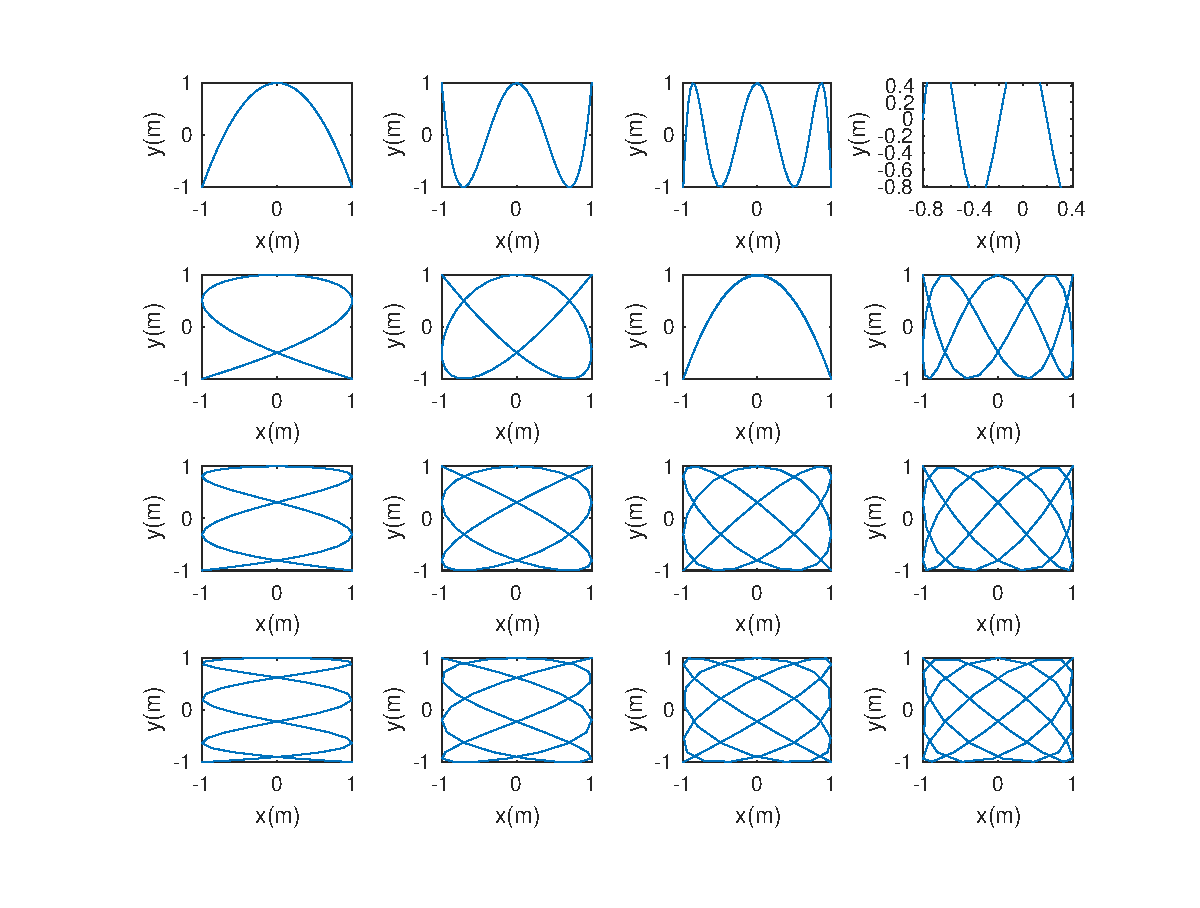
\includegraphics[scale=0.5]{lisa1.eps}
\caption{vista de la figura con los ocho subplots} \label{fig:1}
\end{figure}
